\documentclass{mcmthesis}
\mcmsetup{tcn = 2214713, problem = C, 
	titleinsheet = true, keywordsinsheet = true, titlepage = false}
\usepackage{newtxtext, graphicx, ulem, cite}
\title{\textbf{Certainty amidst Uncertainty: Educated Guesses of Asset Prices and Investment Decisions}}
\author{Chen, Ziyuan \and Chen, Zhirong \and Ma, Zicheng}
\bibliographystyle{abbrv}

\begin{document}
	\begin{abstract}
		
		In this thesis, we tackle the classical yet innovative problem of determining the best trading strategy for two assets with different levels of risk -- gold and bitcoin, of which the bitcoin experiences a much greater extent of fluctuation than gold. This difference in nature suggests specific models to predict their future values and make decisions on trading actions. We perform predictions and decisions before analyzing the model's sensitivity to the commission fee rate. 
		
		Prediction models vary a lot in properties. Since it is only allowed to use historical prices, we divide the time series into two stages -- former 10\% and latter 90\% -- to account for the gradual accumulation of training data. Predictions are made to the prices 1, 7, 15 days from now for later use in decision models. In the former stage, we take \textit{all} historical data into account when predicting and use \textbf{Gray Model (1,1), Past Data Fitting} to depict the general trend out of small training samples. Yet the implied drawbacks are that predictions sometimes blow up at longer timespans (i.e., after 7 days), and higher-order GMs tend to amplify fluctuations. In the latter stage, due to the fixed size of neural network inputs, we use \textbf{Multi-Layer Perceptron, Moving Window Fitting of Past 15 Days} with the assistance of \textbf{dimension rising} to consider price volatility and compensate for the limited window size. Nonetheless, just like the popular ARIMA algorithm, it experiences \textbf{time lag} and makes ``safe'' predictions around the average price. 
		
		In the second part of decision, we establish an improved \textbf{CAPM} (Capital Asset Pricing Model). In order to get a better expected return rate, \textbf{long-term, mid-term and short-term} predicted price data are used to calculate a comprehensive profit. Furthermore, for the purpose of adding the commission fee into the CAPM system, we innovatively combine \textbf{linear programming} and \textbf{risk assessment of portfolio assets}, which transform the decision into a nonlinear programming problem. The improved CAPM model has the ability to guide investors to divide their capital into different assets based on the historical price data. Furthermore, users can customize this model based on their return rate and risk preferences to make it more suitable for them. We also design a lightweight \textit{linear} programming decision model for further simplification while achieving satisfying strategies. 
		
		Finally, we compare different predicted models and decision models, finding that the models yield the best return rate while having the best robustness to different environmental parameters such as commission fee and investor's profit-risk preference (expected profit relative to risk tolerance). After five years, the model can guide investors to earn more than \$30000, which is more than thirty times as in 2016. Such profit mostly comes from the booming price of bitcoin around Spring 2021, which opportunity we successfully seize. 
		
		\begin{keywords}
			Bitcoin; Investment strategy; Gray model; Neural network; CAPM
		\end{keywords}
		
	\end{abstract}
	
	\maketitle
	\newpage
	\tableofcontents
	\newpage
	
	\section{Introduction}
	
	\subsection{Problem Background}
	
	Digital currencies such as bitcoin have been innovative forms of liquidity nowadays, and they are becoming increasingly popular among millions of investors. Unlike most currencies, bitcoin doesn't depend on a specific issue, but on a specific algorithm. It makes use of the P2P network composed of many nodes in a distributed database to identify and record all transactions, and utilizes cryptography to guarantee the security of each trading link at the same time. 
	
	Plenty of evidence shows that the number of bitcoin investors is growing nonlinearly \cite{INVESTOR}. The data collected by global analytics and advice firm Gallup revealed that the proportion of investors in the U.S. holding bitcoin has jumped from 2\% in 2018 to 6\% in June 2021 -- almost 3 times as before. However, according to Kyriazis, a financial scholar at the University of Thessaly, whether bitcoin can be characterized as a good (like gold) or fiat money (like the dollar) is still uncertain in the near future. In the following, we will briefly analyze the characteristics of gold and bitcoin. 
	
	As one of the most malleable, dense, conductive, and beautiful metals in the world, gold is viewed as the most representative hedge or haven against volatility in the world. According to Baur and Lucey, hedges are financial assets with little correlation with alternative assets. Therefore, when there is a big fluctuation in the financial market, they can serve as havens for investors. 
	
	Gold is traded in a well-regulated market with a long history, and its price fluctuates mildly around several thousand. On the contrary, bitcoin is the product of blockchain technology and has a relatively self-organized market. Its price is highly volatile due to a lack of regulation measures, ranging from \$600 to \$63,500 with two major appreciations in Winter 2018 and Spring 2021. 
	
	Compared to gold, bitcoin is a highly decentralized digital currency with nearly no intrinsic value, which is regarded as a kind of innovative payment. Nevertheless, The price of bitcoin is on a roller-coaster ride as speculators step in, making it more suitable for speculation than for anonymous trading. Furthermore, researchers have revealed that there is a weak nexus between bitcoin and gold -- in other words, gold is far from being a haven in the asset market. Therefore, choosing a balanced investment strategy between gold and bitcoin is hard for most investors. 
	
	\subsection{Literature Review}
	
	Thousands of bitcoin and gold price prediction methods have been thoroughly researched by scholars all over the world, whereas only a few of them predict the price based only on historical price data. As for bitcoins, previous research indicated that \textbf{neural networks} \cite{NN} and \textbf{time series models} \cite{TSA} are mostly used in the past five years. However, the biggest challenge is that these models can either predict the bitcoin price ahead of only a short time, or make a long-term prediction with unsatisfying accuracy. Additionally, for now, nearly no scholar has researched bitcoin prediction with short-term historical data. We innovatively tackle the problem by (1) developing \textbf{Gray Models} on short-term data and (2) combining different algorithms during various stages in the time series to achieve both long-term and short-term prediction. 
	
	As for the allocation of our capital into different assets, one of the most famous theories is \textbf{CAPM} (Capital Asset Pricing Model). The model tells us how to appraise the asset based on its risk and yield rate. Its key point is to explore the quantitative relationship between profit and risk -- that is, how much profit investors would get while compensating for a certain degree of risk. 
	
	\subsection{Problem Restatement and Our Approach}
	
	For this problem, we are offered two datasets containing the prices of bitcoin and gold. Our target is to develop a model to help traders decide whether to buy, hold, or sell their assets each day based solely on data from previous days. The requirements can be broken down as follows:
	\begin{enumerate}
		\item[$\bullet$] Construct a model based only on past data series to determine the best trading strategy. 
		\item[$\bullet$] Prove that the proposed method yields the best strategy.
		\item[$\bullet$] Determine model sensitivity in varying commission fees. 
	\end{enumerate}
	
	In our approach, the task is therefore divided into three parts: 
	\begin{enumerate}
		\item \textbf{Prediction}: We divide the whole time series into the short-term and long-term stages. ``Short-term'' indicates a lack of data, while ``long-term'' means the accumulation of available data as time goes by. We develop different prediction methods in the two stages.
		\item \textbf{Decision}: Our decision models are build based on \textbf{CAPM}. We put forward a new method to measure return rate considering both short-term and long-term gains. Different weights are added to construct an indicator to represent prospective earnings. Based on predicted future prices, a nonlinear programming model is used to find the balance between profit and risk.
		\item \textbf{Senstivity analysis}: Changing commission fee rates allow us to analyze the model's robustness. Although final earnings may differ, the trends of value growth are similar. 
	\end{enumerate}

	\begin{figure}[h]
		\centering 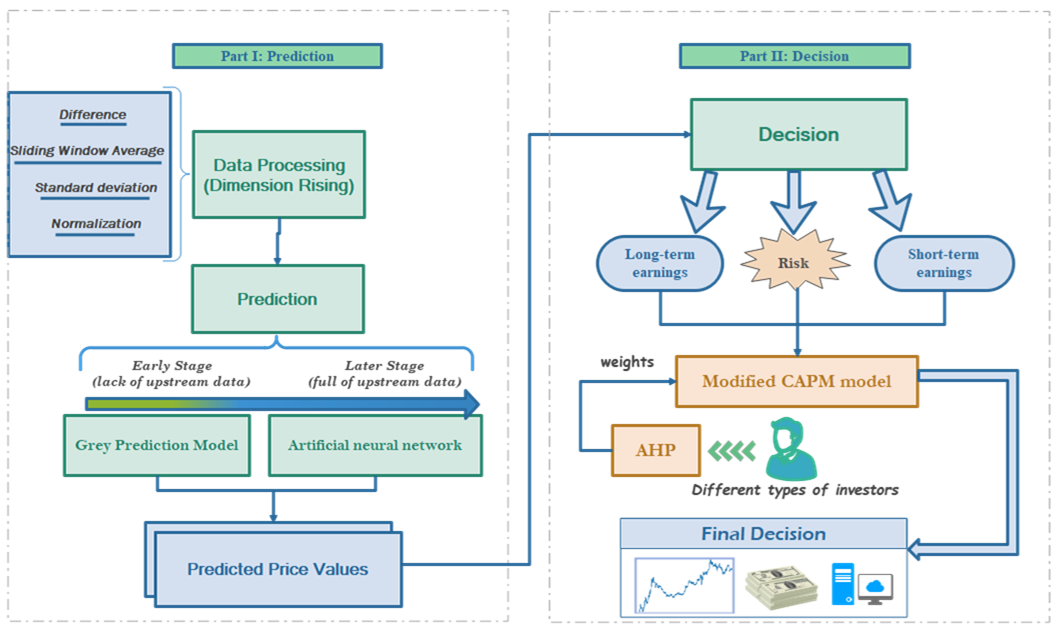
\includegraphics[width=12cm]{GlobalFlowChart}
		\caption{Flow chart of the complete problem analyzing and solving process}
	\end{figure}
	
	\section{Model Preparation}
	
	\subsection{Assumptions and Justifications}
	\begin{itemize}
		\item \textbf{Assumption 1}: 
		In the absence of enormous changes in society, the prices of gold and bitcoin show a weak correlation. 
		\\ $\hookrightarrow$ Justification: 
		Previous studies suggest that bitcoin is more subject to uncertainty at lower and higher quantiles, while gold remains stable with \textbf{smaller hedges and safe-haven coefficients}. Additionally, Kendall's $\tau_b$ correlation coefficient between the prices is only \textbf{0.558}, which indicates the relationship between gold and bitcoin is weak (considering that both bitcoin and gold experiences dollar inflation). To be specific, the bitcoin price is stable while the gold price goes up, and vice versa (refer to the two ``branches'' in Figure 2). 
		
		\begin{figure}[h]
			\centering 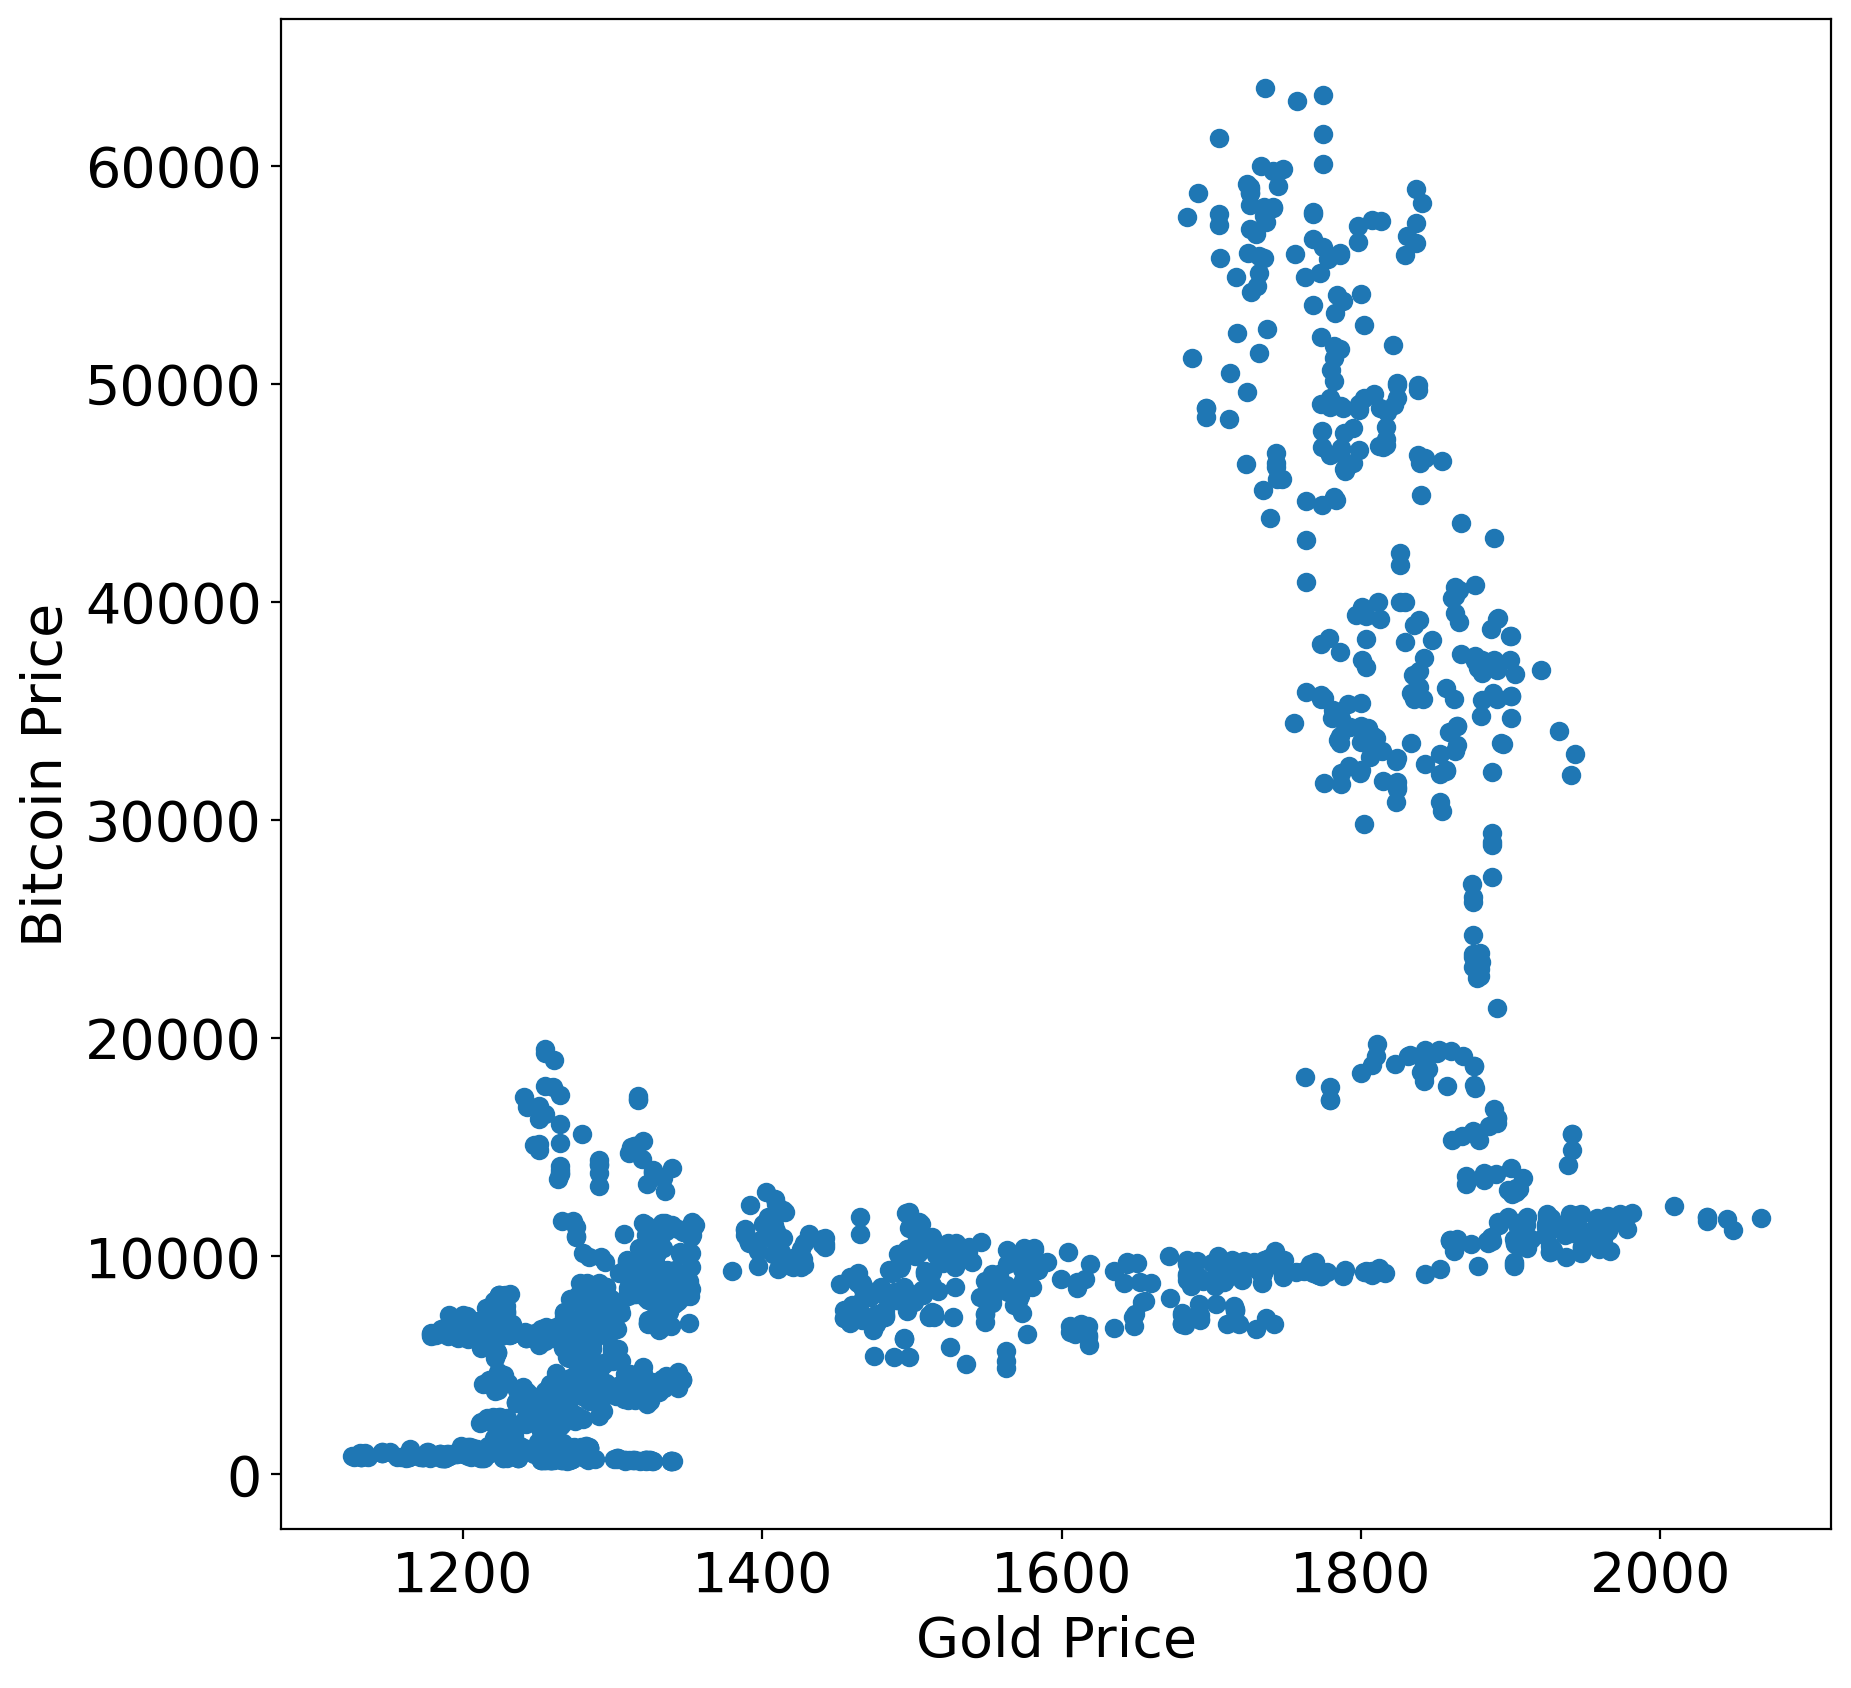
\includegraphics[width=8cm]{PriceCorr}
			\caption{Scatter plot of gold ($x$-axis) and bitcoin ($y$-axis) prices ($R^2$-score = 0.546569)}
		\end{figure}
		
		\item \textbf{Assumption 2}: 
		Transactions by the investor have no influence on the gold and bitcoin prices. 
		\\ $\hookrightarrow$ Justification: 
		Since large numbers of transactions are made every day, the influence of a single investor is too trivial to be considered. 
		
		\item \textbf{Assumption 3}: 
		The current bitcoin price and gold price are based only on historical price data and are independent of external factors. 
		
		\item \textbf{Assumption 4}: 
		Only \textit{profit} and \textit{risk} play as the main factors affecting investment decisions. 
		
		\item \textbf{Assumption 5}: 
		All of the investors follow the dominance rule; that is, under the same level of risk, investors should 
		select the asset with a higher yield. 
		
		\item \textbf{Assumption 6}: 
		There is no limit for the transaction amount of gold and bitcoin. 
	\end{itemize}
		
	\subsection{Symbols and Notations}
	\begin{center}
		\begin{tabular}{clc}
			\toprule
			Symbol & Description & Unit \\ \midrule
			$C, G, B$ & Open interest -- Cash, Gold, Bitcoin & \$ \\
			$\Delta G, \Delta B$ & Trading volume -- Gold, Bitcoin & \$ \\
			$p_{G-x}, p_{B-x}$ & Actual price (before $x$ days) -- Gold, Bitcoin ($x = 0,1,2,\ldots$) & \$ \\
			$p_{G}, p_{B}$ & Actual price (today) -- Gold, Bitcoin & \$ \\
			$p_{G+1}, p_{B+1}$ & Actual price (tomorrow) -- Gold, Bitcoin & \$ \\
			$\hat{p}_{G+x}, \hat{p}_{B+x}$ & Predicted price (after $x$ days) -- Gold, Bitcoin ($x = 1,7,15$) & \$ \\
			$\alpha_{G}, \alpha_{B}$ & Rate of commission in each transaction -- Gold, Bitcoin & \\
			$\sigma_{G}, \sigma_{B}$ & Standard deviation of price (past 15 days) -- Gold, Bitcoin & \$ \\
			$E_{G}, E_{B}$ & Expected profit rate -- Gold, Bitcoin & \\
			$\beta_{x}$ & Weight coefficients in expected profit rate ($x = 1,2,3$) & \\
			$\rho$ & Correlation coefficient of gold and bitcoin prices & \\
			$r$ & Investor's Vulnerability Index: lower $r$ means higher risk tolerance & \\
			$\omega$ & Balance Ratio: portion of gold in the total asset (gold \& bitcoin) & \\
			$K$ & Sharp Ratio: ratio of profit (by appreciation) to risk (by stdev) & \\
			$\textbf{\textrm{X}}_{opt}$ & The optimal value of the variable $\textbf{\textrm{X}}$ & \\
			\bottomrule
		\end{tabular}
	\end{center}
	
	\subsection{Data Cleaning and Preprocessing}
	
	Due to the absence of additional datasets and single dimensionality (as ``prices''), data cleaning takes up relatively little time in the model's development. In order to simplify the problem, gold ``prices'' in market closing days are obtained through the forward \textbf{padding} method. Both the market closing days and the commission fees are factors that are omitted in the initial model assumptions and are gradually added as the model complexifies. 
	
	The role of data preprocessing, on the contrary, is far from trivial. As discussed in detail in Section \ref{sec:3.3}, \textbf{dimension rising} is applied to obtain criteria reflecting long-term characteristics accompanying a single day's data. These data can have useful implications: the average price over the past 15 days indicates the trend and potential gain, while the standard deviation and (first- or second-order) difference indicates instability and hidden risks. In the CAPM model, changes in these criteria can affect the parameters reflecting investors' preferences like expected gain and risk tolerance. Moreover, data must be \textbf{normalized} or \textbf{min-max scaled} before being applied to CAPM. 
		
	\newpage
	\section{Problem I: Predicting Future Prices of Gold and Bitcoin}
	
	\subsection{Former Stage, Short-Term: Gray Model Prediction (GM)}
	
	Gray model is a newly investigated model that makes use of \textit{generated} series -- usually an accumulation of original data -- and is especially effective for predicting based on a small amount of data. At the beginning of the given time series, it is capable of predicting the price of gold and bitcoin based on either the complete data from history (PDF) or data from last week (MWF-7). Note that since PVA accumulates error (as in Section \ref{sec:3.1}), \textbf{all the following models, unless specially noted, incorporates AVA in moving window fitting.}
	
	\begin{figure}[h]
		\label {fig:3}
		\centering 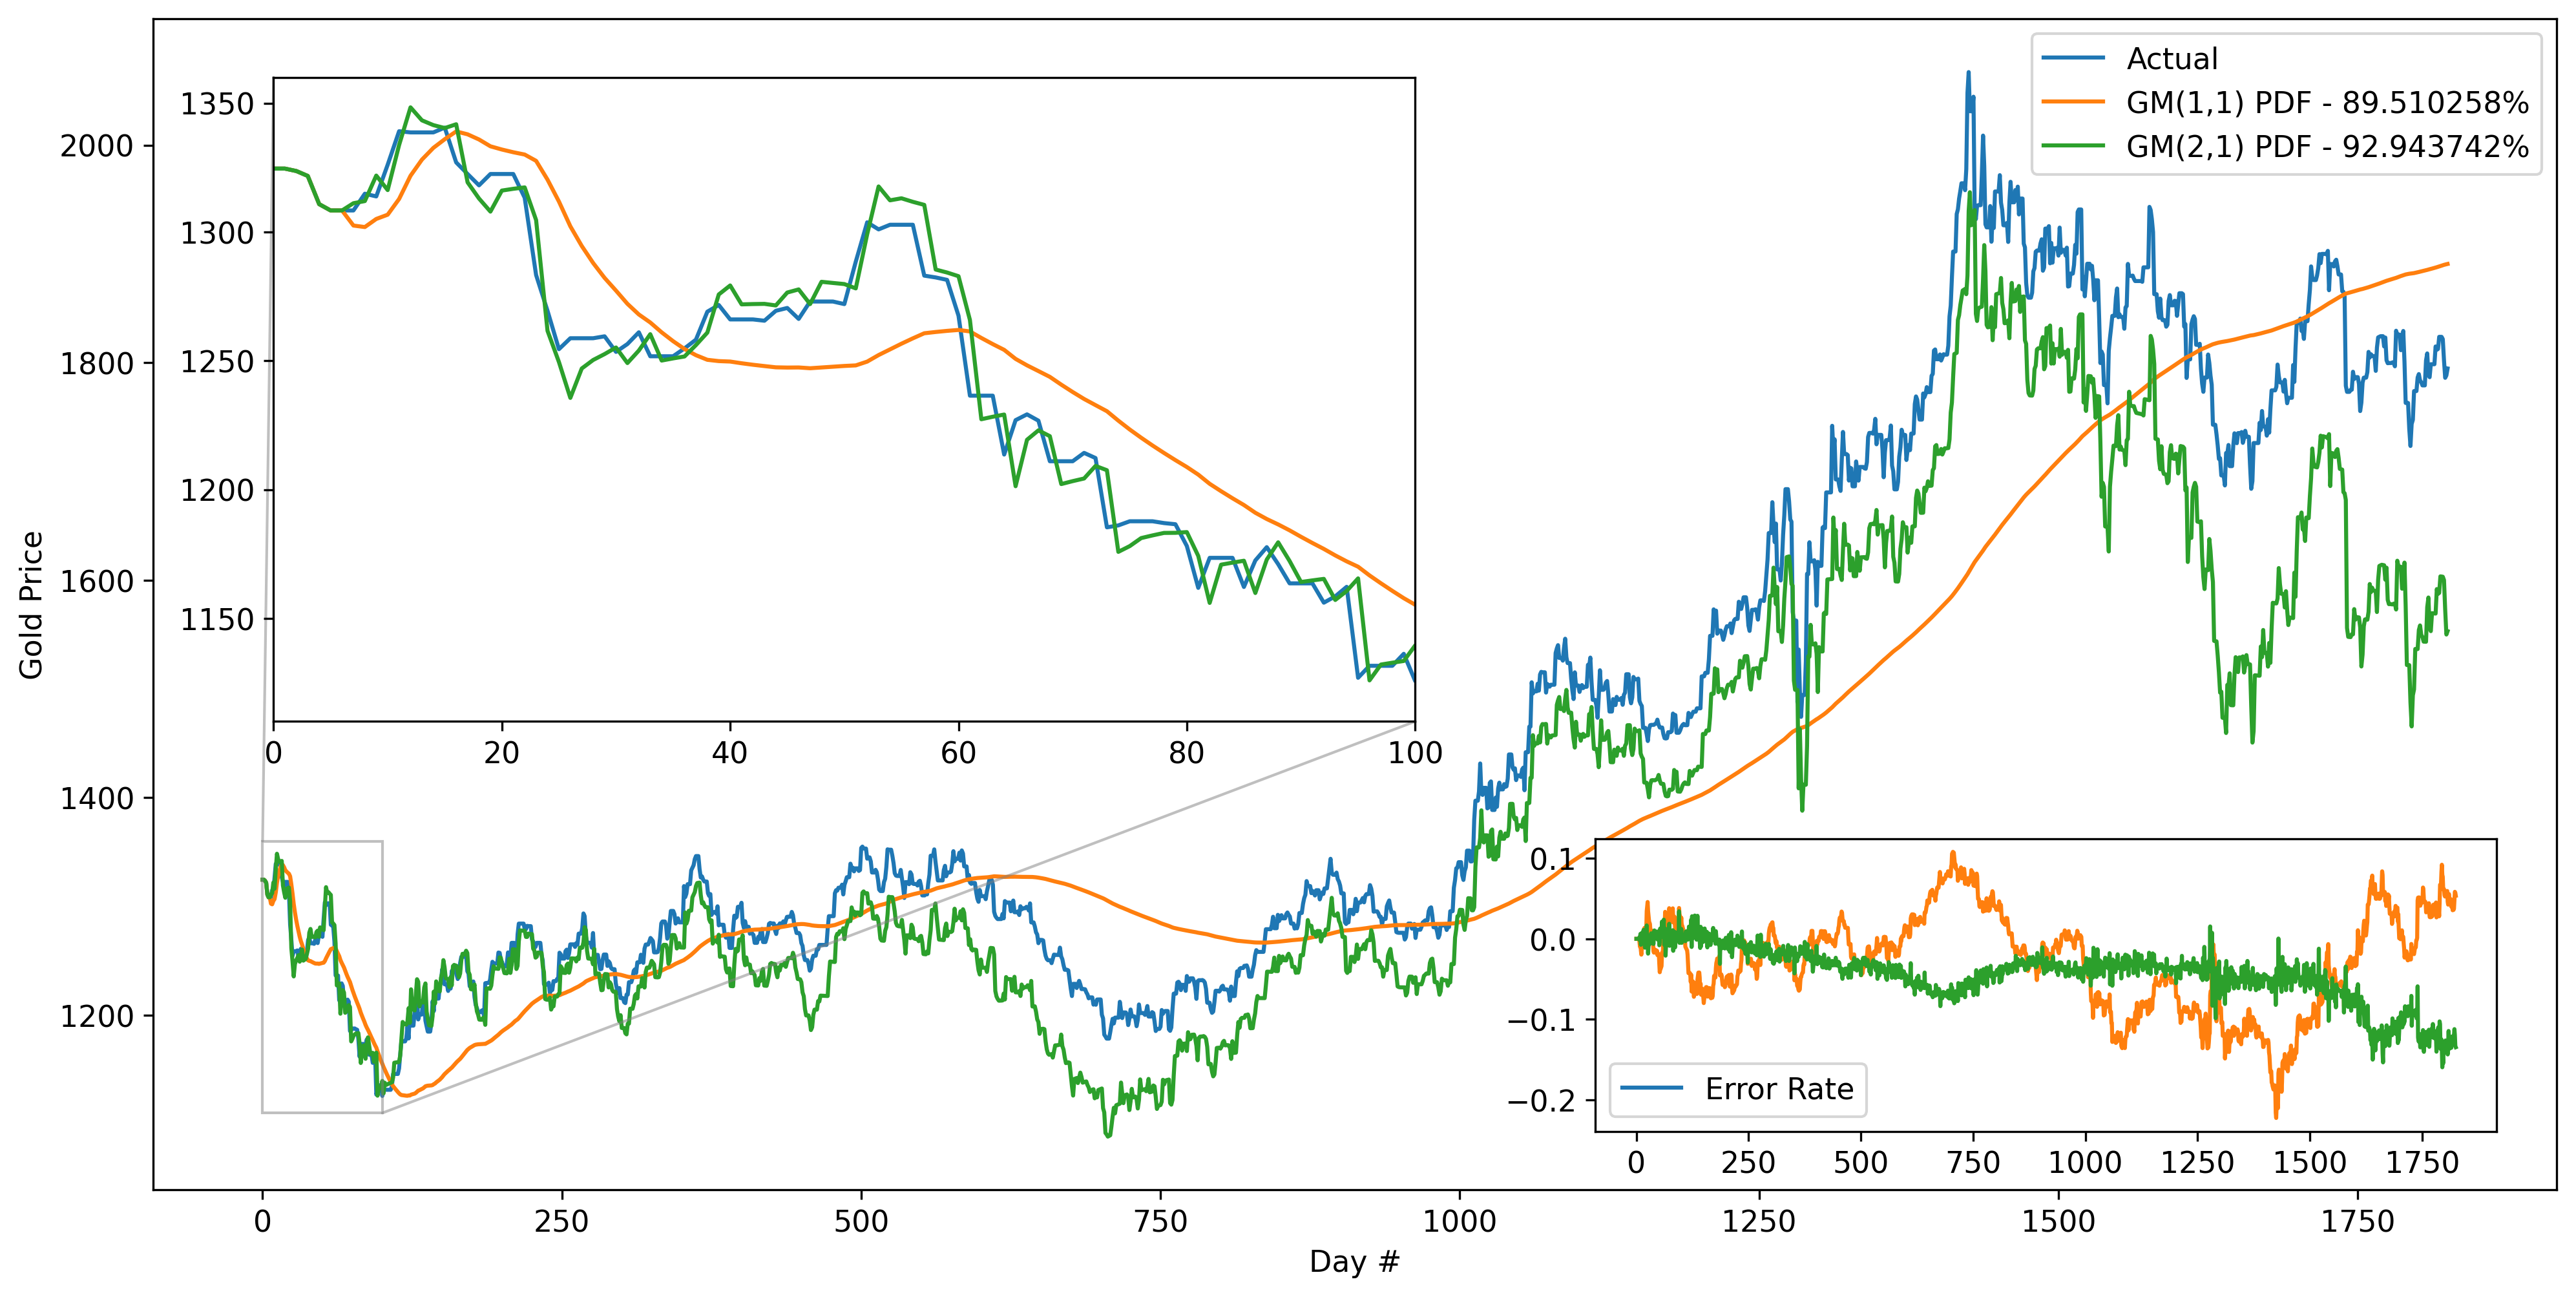
\includegraphics[width=11.6cm]{GMGold}
		\centering 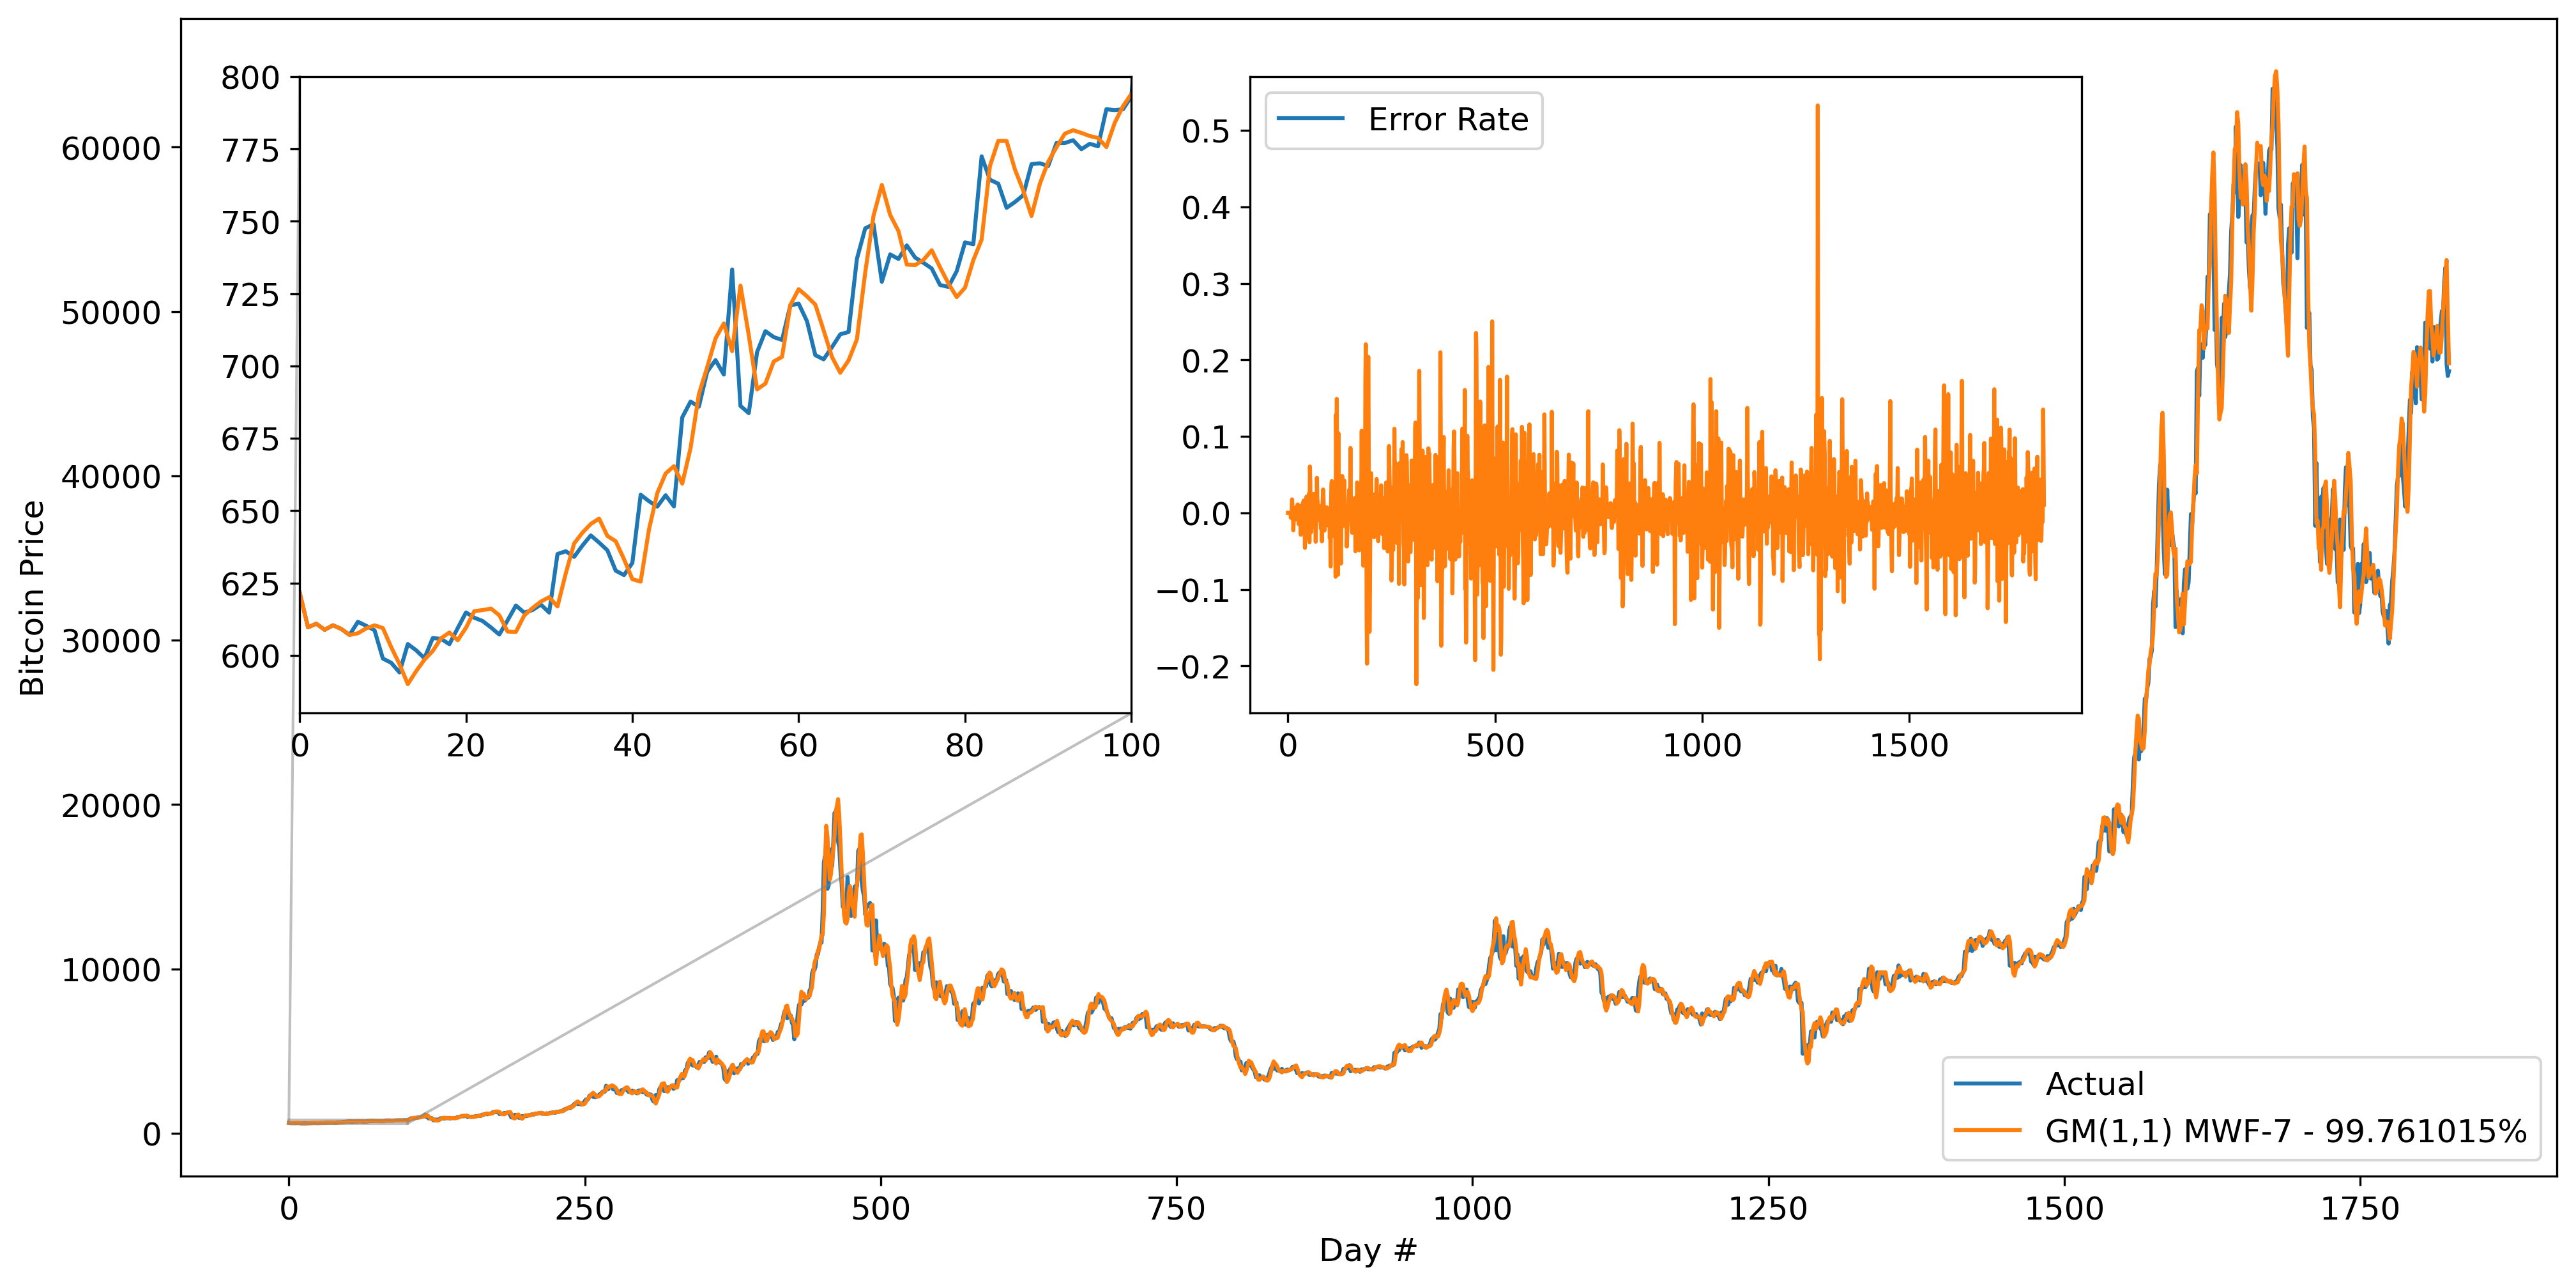
\includegraphics[width=11.6cm]{GMBitcoin}
		\caption{GM prediction of gold (top) and bitcoin (bottom) prices, starting from Day \#7}
	\end{figure}
	
	Some model selection is performed in this process. GM(1,1) PDF, GM(2,1) PDF, and GM(2,1) MWF-7 goes into the negative region when predicting bitcoin prices, and GM(1,1) MWF-7 fails to run on gold prices. But the available GMs are sufficient for use: the absolute error rates are 5.209258±4.153883\%, 4.496556±3.178538\%, and 3.578030±3.799295\%, respectively. GM(1,1) model sketches the general trend of the series, while GM(2,1) depicts the shape with more details. 
	
	Nonetheless, as the zoomed part indicates, GM is not free from the time lag. The largest obstacle in incorporating GM is its restrictions on the varying rates of data: it works best on exponentially growing data and worst on acutely fluctuating data. To some extent, this time lag is caused by the ``momentum'' of growth -- a closer examination on the error rates reveals that the prediction most severely deviates from the actual value at sharp turning points. Yet this hardly affects GM's pragmatic value: sharp turns usually originate from spontaneous mass trading (with the absence of a ``circuit breaker'') not represented in historical prices. 
	
	\subsection{Latter Stage, Short-Term: Time Series Analysis (ARIMA)}
	\label{sec:3.1}
	
	At first sight, time series analysis seems to be the golden algorithm for this problem. It looks for hidden patterns inside both stable and unstable time series. The most popular model, ARIMA, achieves this through means of AR (autoregression), I (Integration), and MA (moving average). Other models such as Holt-Winters take seasonal fluctuations into account, yet it is unsuitable for this problem since the rise and fall of financial assets' prices are not embedded with a highly seasonal pattern except for some major events, whose presence can hardly be predicted in advance. Therefore, we incorporate ARIMA as an initial approach to the price prediction problem. 
	
	Nonetheless, the module function of \verb|statsmodels.api.tsa.ARIMA| in Python produces predictions for a single point of time based on the \textit{whole} series -- in a sense, it is better to be called \textit{regression} than prediction. Such an approach is referred to as \textbf{Global Data Fitting} in our paper. Taking the requirement of predicting "only on price data up to that day" into account, we refine the algorithm in a way such that only \textbf{Past Data Fitting} is used to calculate the current value. While predicting based on the entire set of past data can be accurate, it cannot always be achieved in real life due to a lack of data source or computing power. Therefore, an alternative approach is \textbf{Moving Window Fitting} with a certain window size $x$. As the window moves, either an actual value or a newly predicted value can be added to maintain the window size. These two options are referred to as \textbf{Actual Value Aided} and \textbf{Predicted Value Aided}, respectively. 
	
	\begin{center}
		\begin{tabular}{cl}
			\toprule
			Abbrev. & Description \\ \midrule
			\textbf{GDF} & Global Data Fitting \\
			\textbf{PDF} & Past Data Fitting \\
			\textbf{MWF-$x$} & Moving Window Fitting of Size $x$ \\
			\textbf{AVA} & Actual Value Aided \\
			\textbf{PVA} & Predicted Value Aided \\
			\bottomrule
		\end{tabular}
	\end{center}
	
	\begin{figure}[h]
		\centering 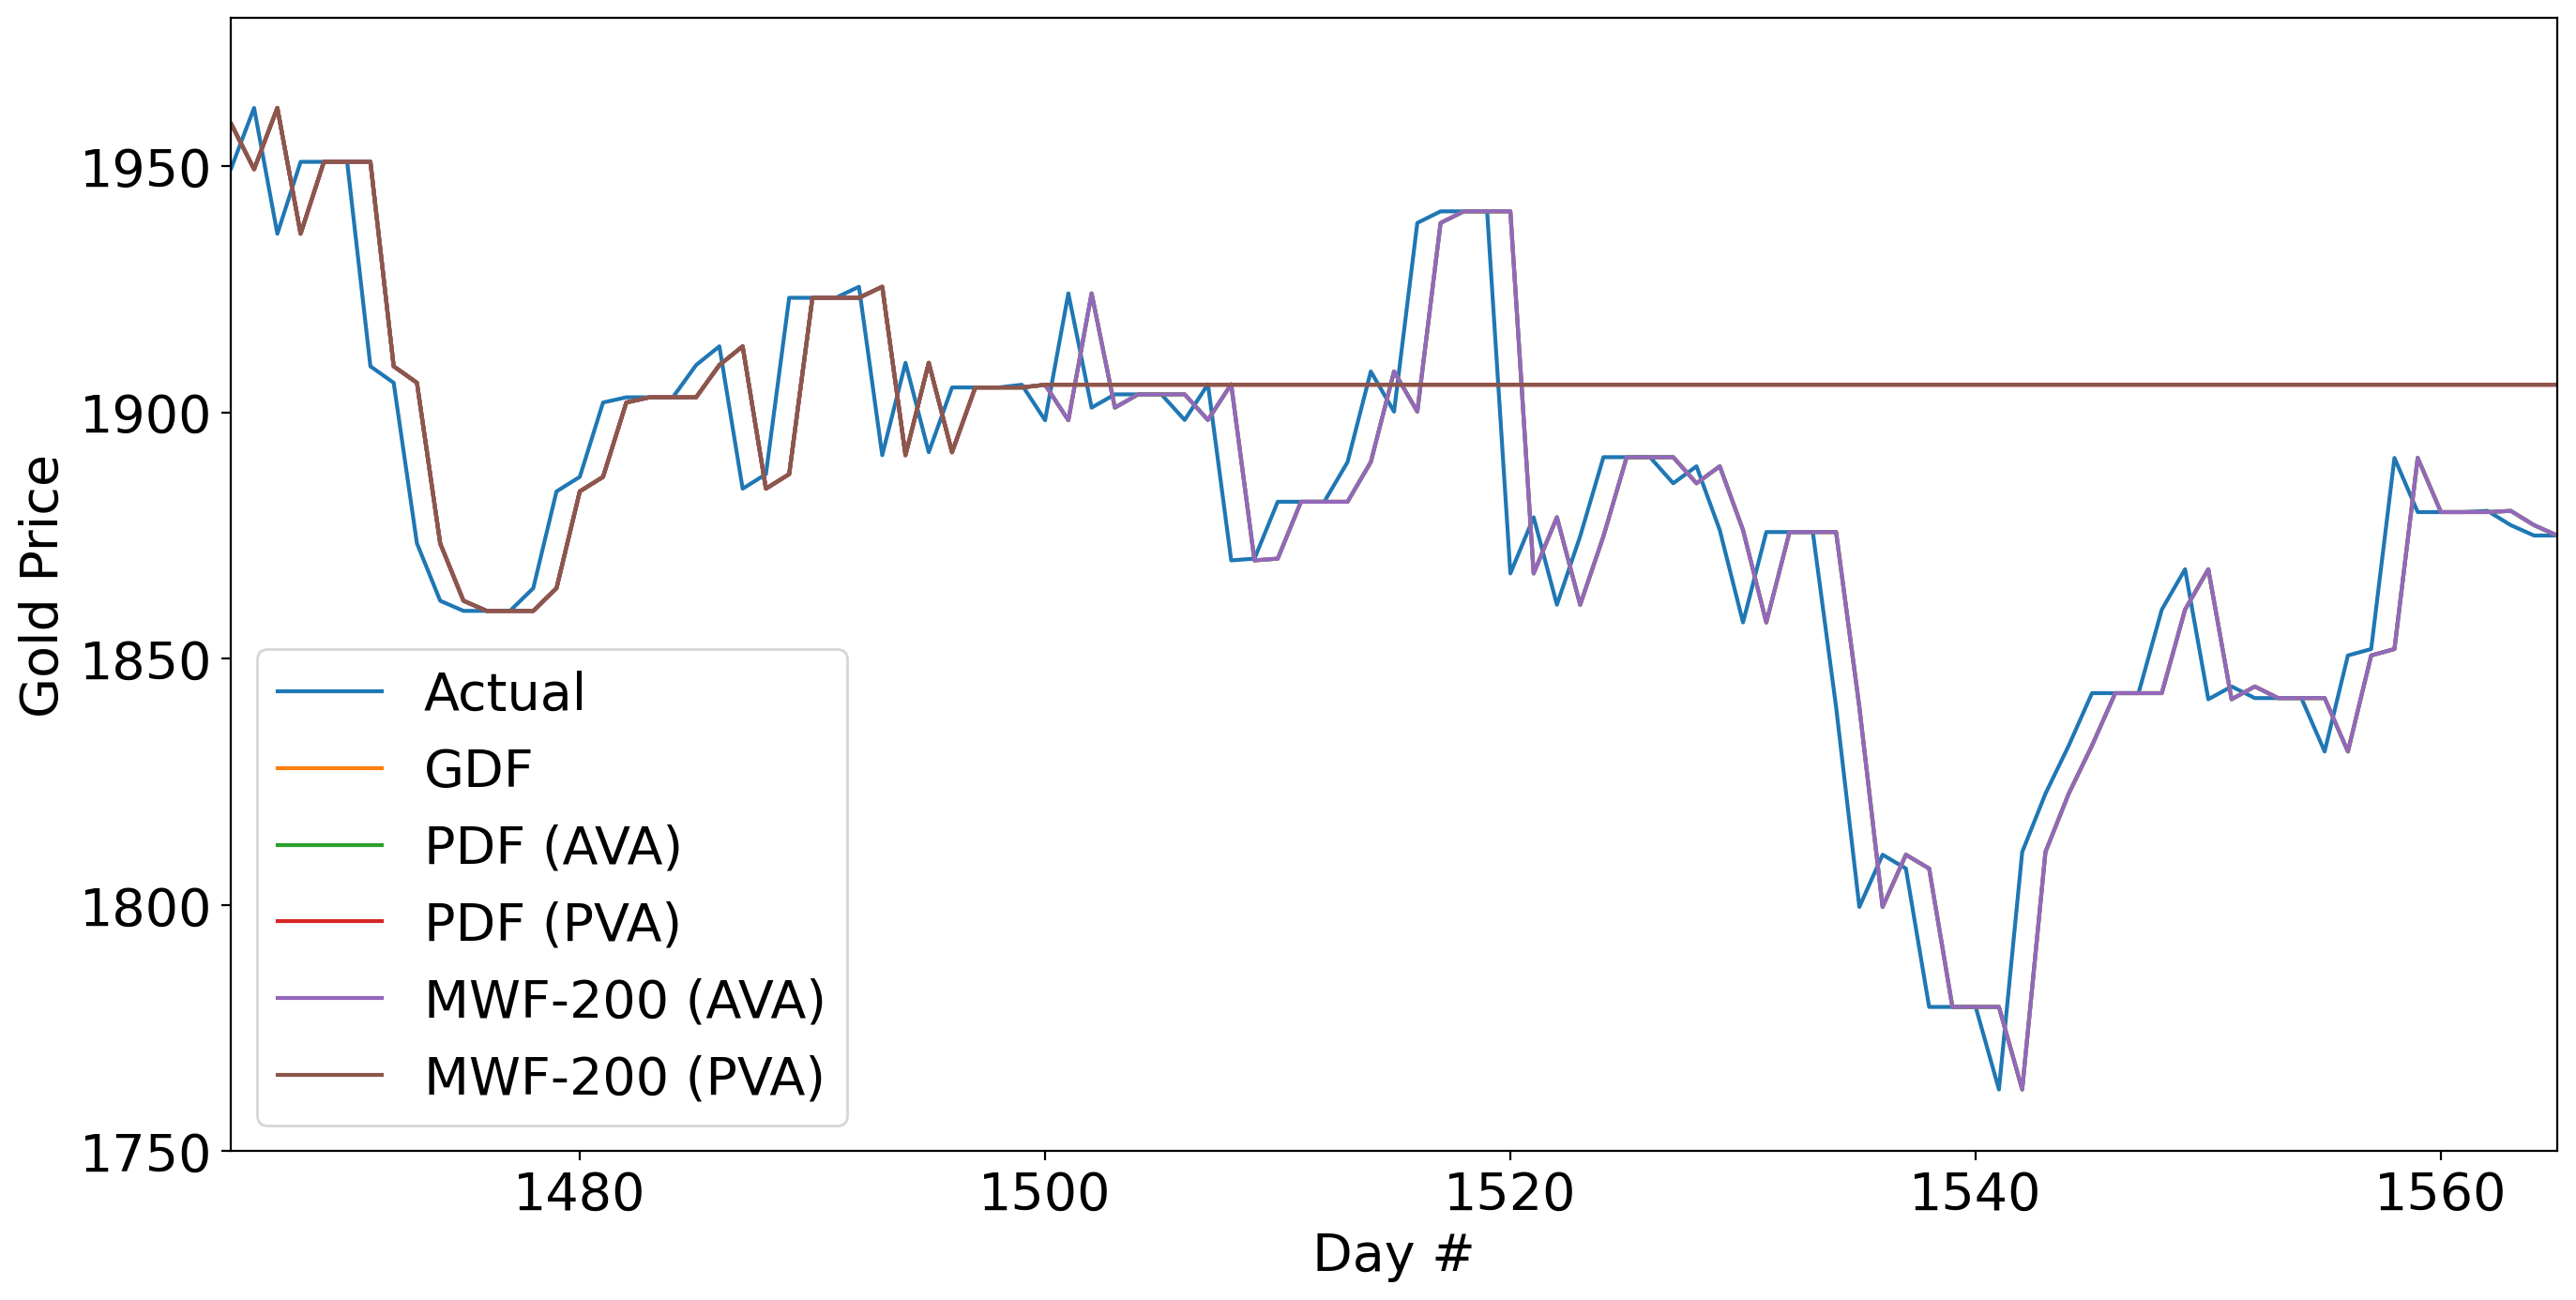
\includegraphics[width=8.1cm]{ArimaGold}
		\centering 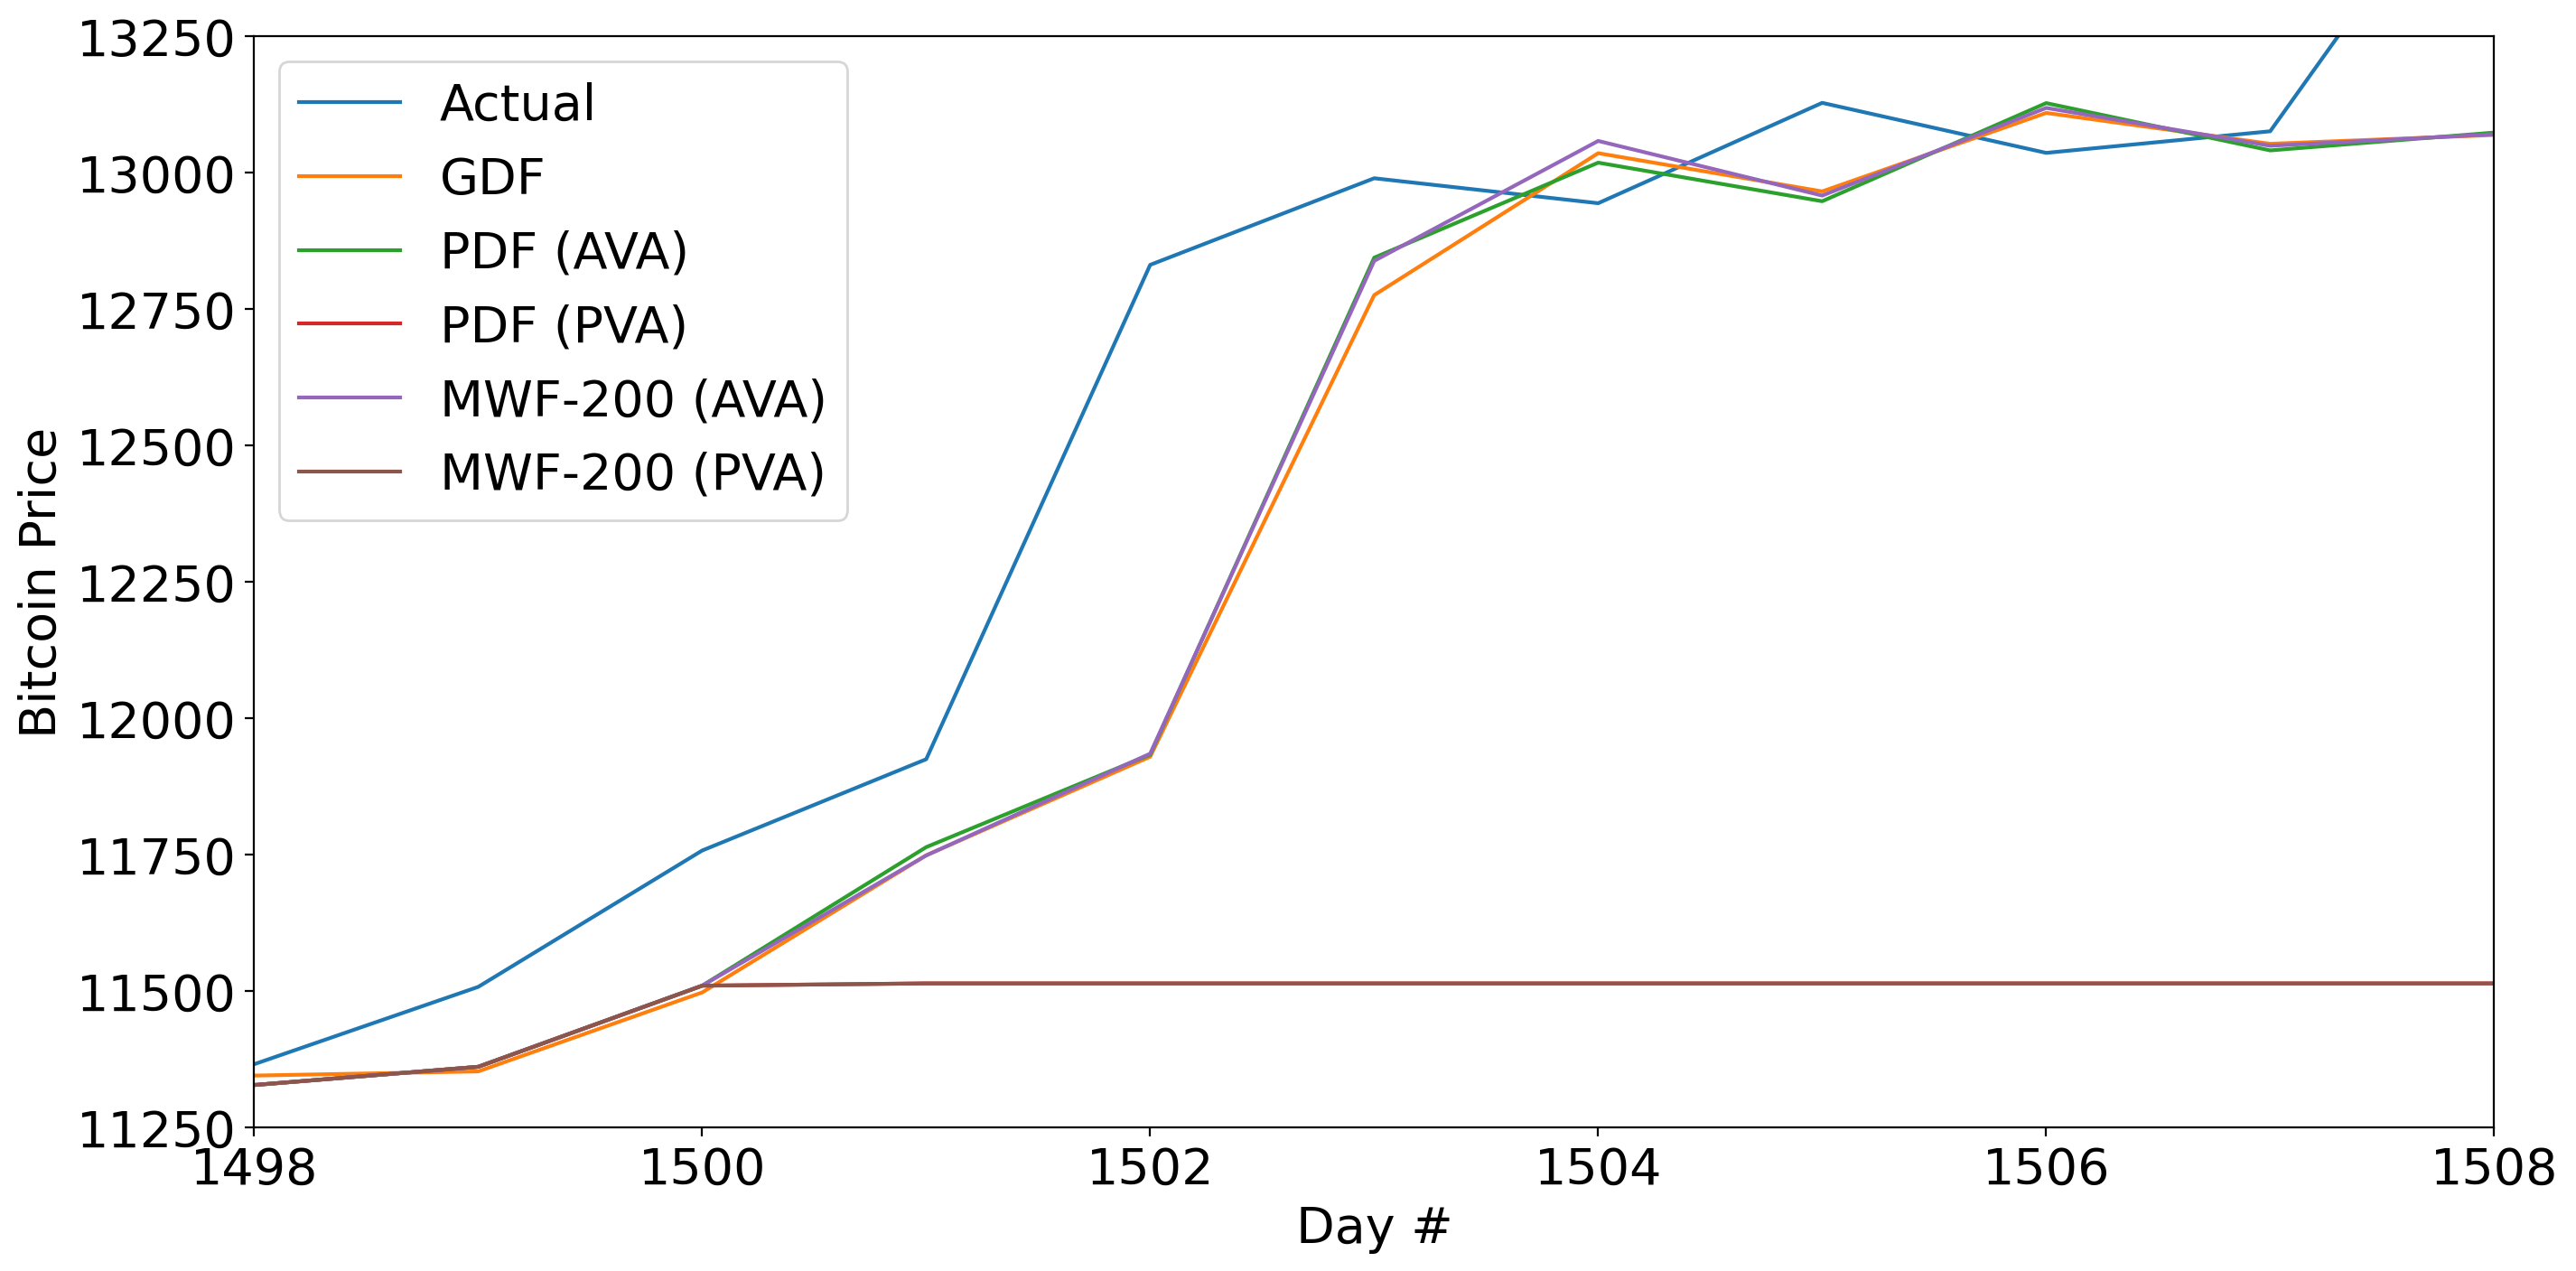
\includegraphics[width=8.2cm]{ArimaBitcoin}
		\caption{ARIMA prediction of gold (left) and bitcoin (right) prices, starting from Day \#1500}
	\end{figure}
	
	As is evident from the charts, one severe drawback of ARIMA is the \textbf{time lag} -- in this case, by one time unit. In other words, although the models of gold (ARIMA(0,1,0)) and bitcoin (ARIMA(0,1,2)) achieve 99.893041\% and 99.836086\% accuracy respectively in fitting the training series, it merely copies the previous data as prediction despite some minor adjustments. Such a phenomenon is similar to the overfitting issue in machine learning \cite{OVERFIT}: the model struggles to fit the training data perfectly while overseeing the general characteristics. Therefore, ARIMA is only suitable for performing extremely short-term predictions lasting for one day or two. Also, note that PVA fails to produce sensible predictions due to the accumulation of error at each step. 
	
	\subsection{Latter Stage, Long-Term: Artificial Neural Network (MLP, SVM)}
	\label{sec:3.3}
	
	When data become sufficient as time goes by, machine learning becomes an effective approach in constructing a model from massive data \cite{ML}. We incorporate the Multi-Layer Perceptron (MLP) and Support Vector Machine (SVM). More complex networks fine-tuned for ``remembering'' historical data like Long-Short Term Memory Network (LSTM) may be applicable with further research \cite{LSTM}. 
	
	\begin{figure}[h]
		\centering 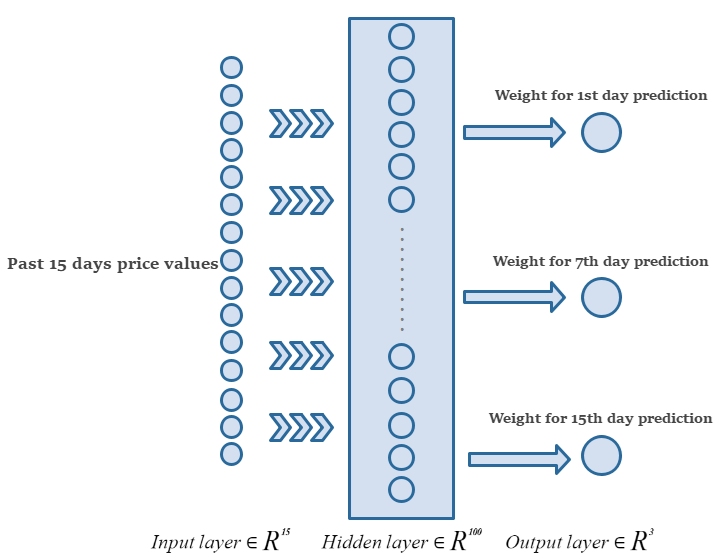
\includegraphics[width=14.4cm]{NeuralNetwork}
		\caption{The network structure diagram of Multi-Layer Perceptron}
	\end{figure}
	
	\textbf{MLP} is a kind of lightweight yet predictive neural network. With the learning rate of 0.001, ReLU activation, and hidden layer size of 100, we first perform rolling prediction on both given series to determine the best initial window size among the choices of 1 (0.999462 / 0.998875), 3 (0.963185 / 0.997142), 5 (0.994998 / 0.994698), 7 (0.988270 / 0.992314), and 9 (0.984009 / 0.991178). $R^2$ relevance scores are shown the parentheses. 
	
	\begin{figure}[h]
		\centering 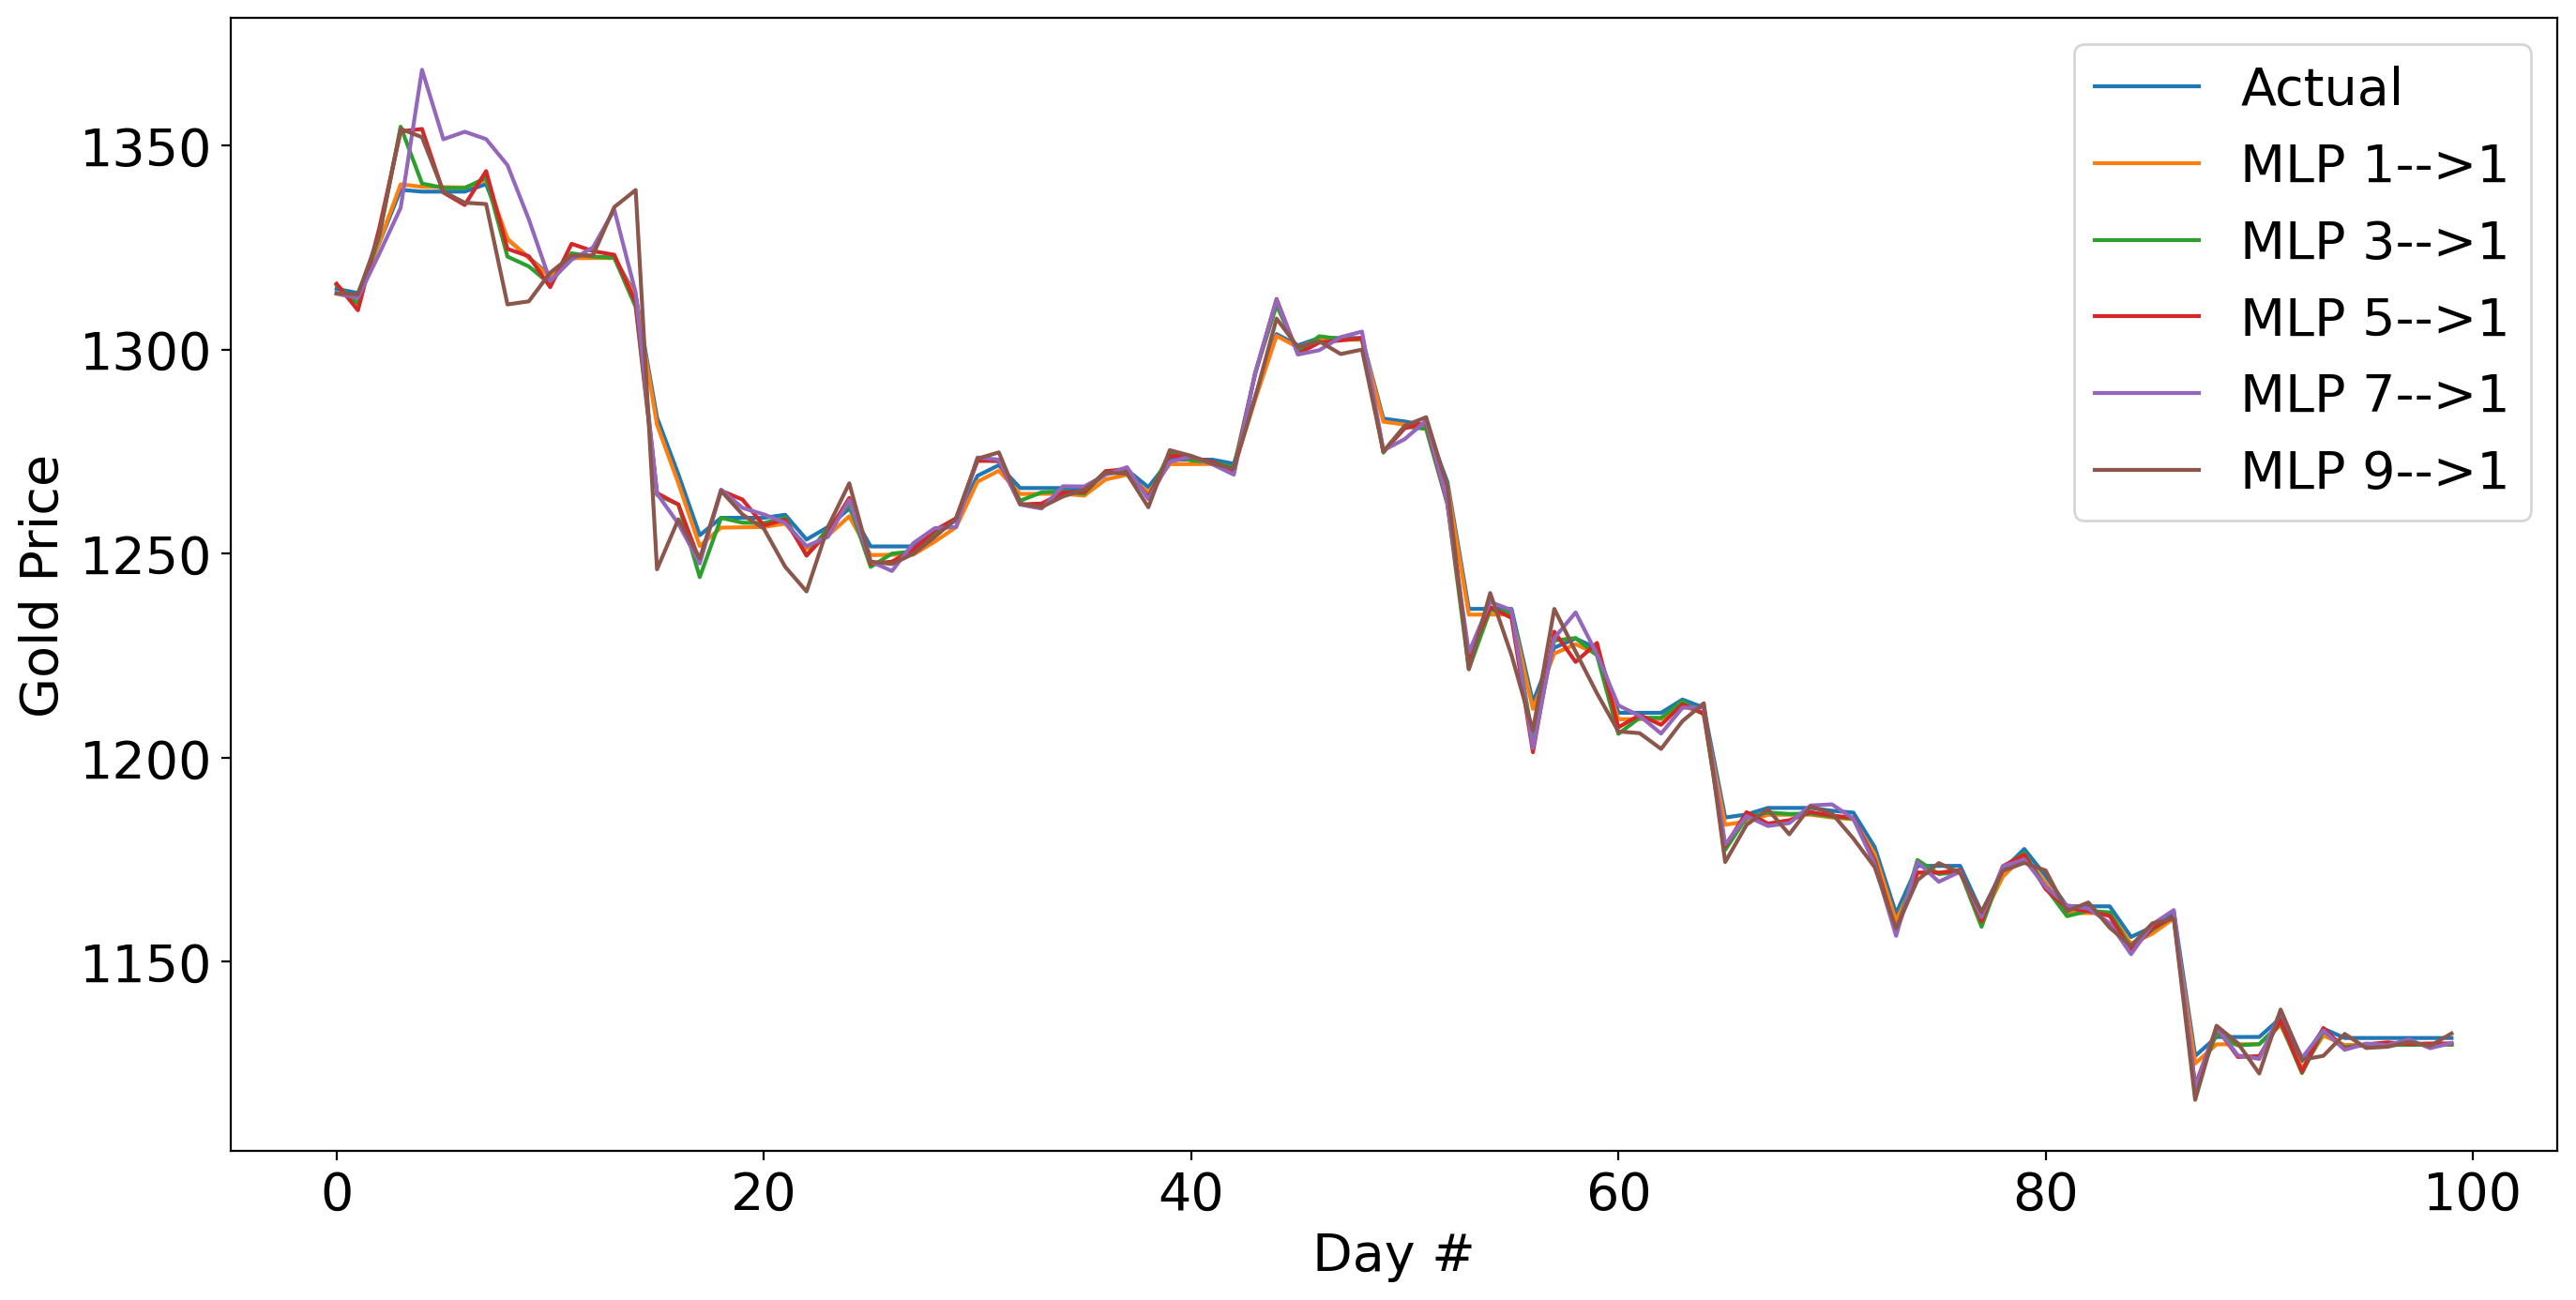
\includegraphics[width=8.1cm]{MLPGoldRoll}
		\centering 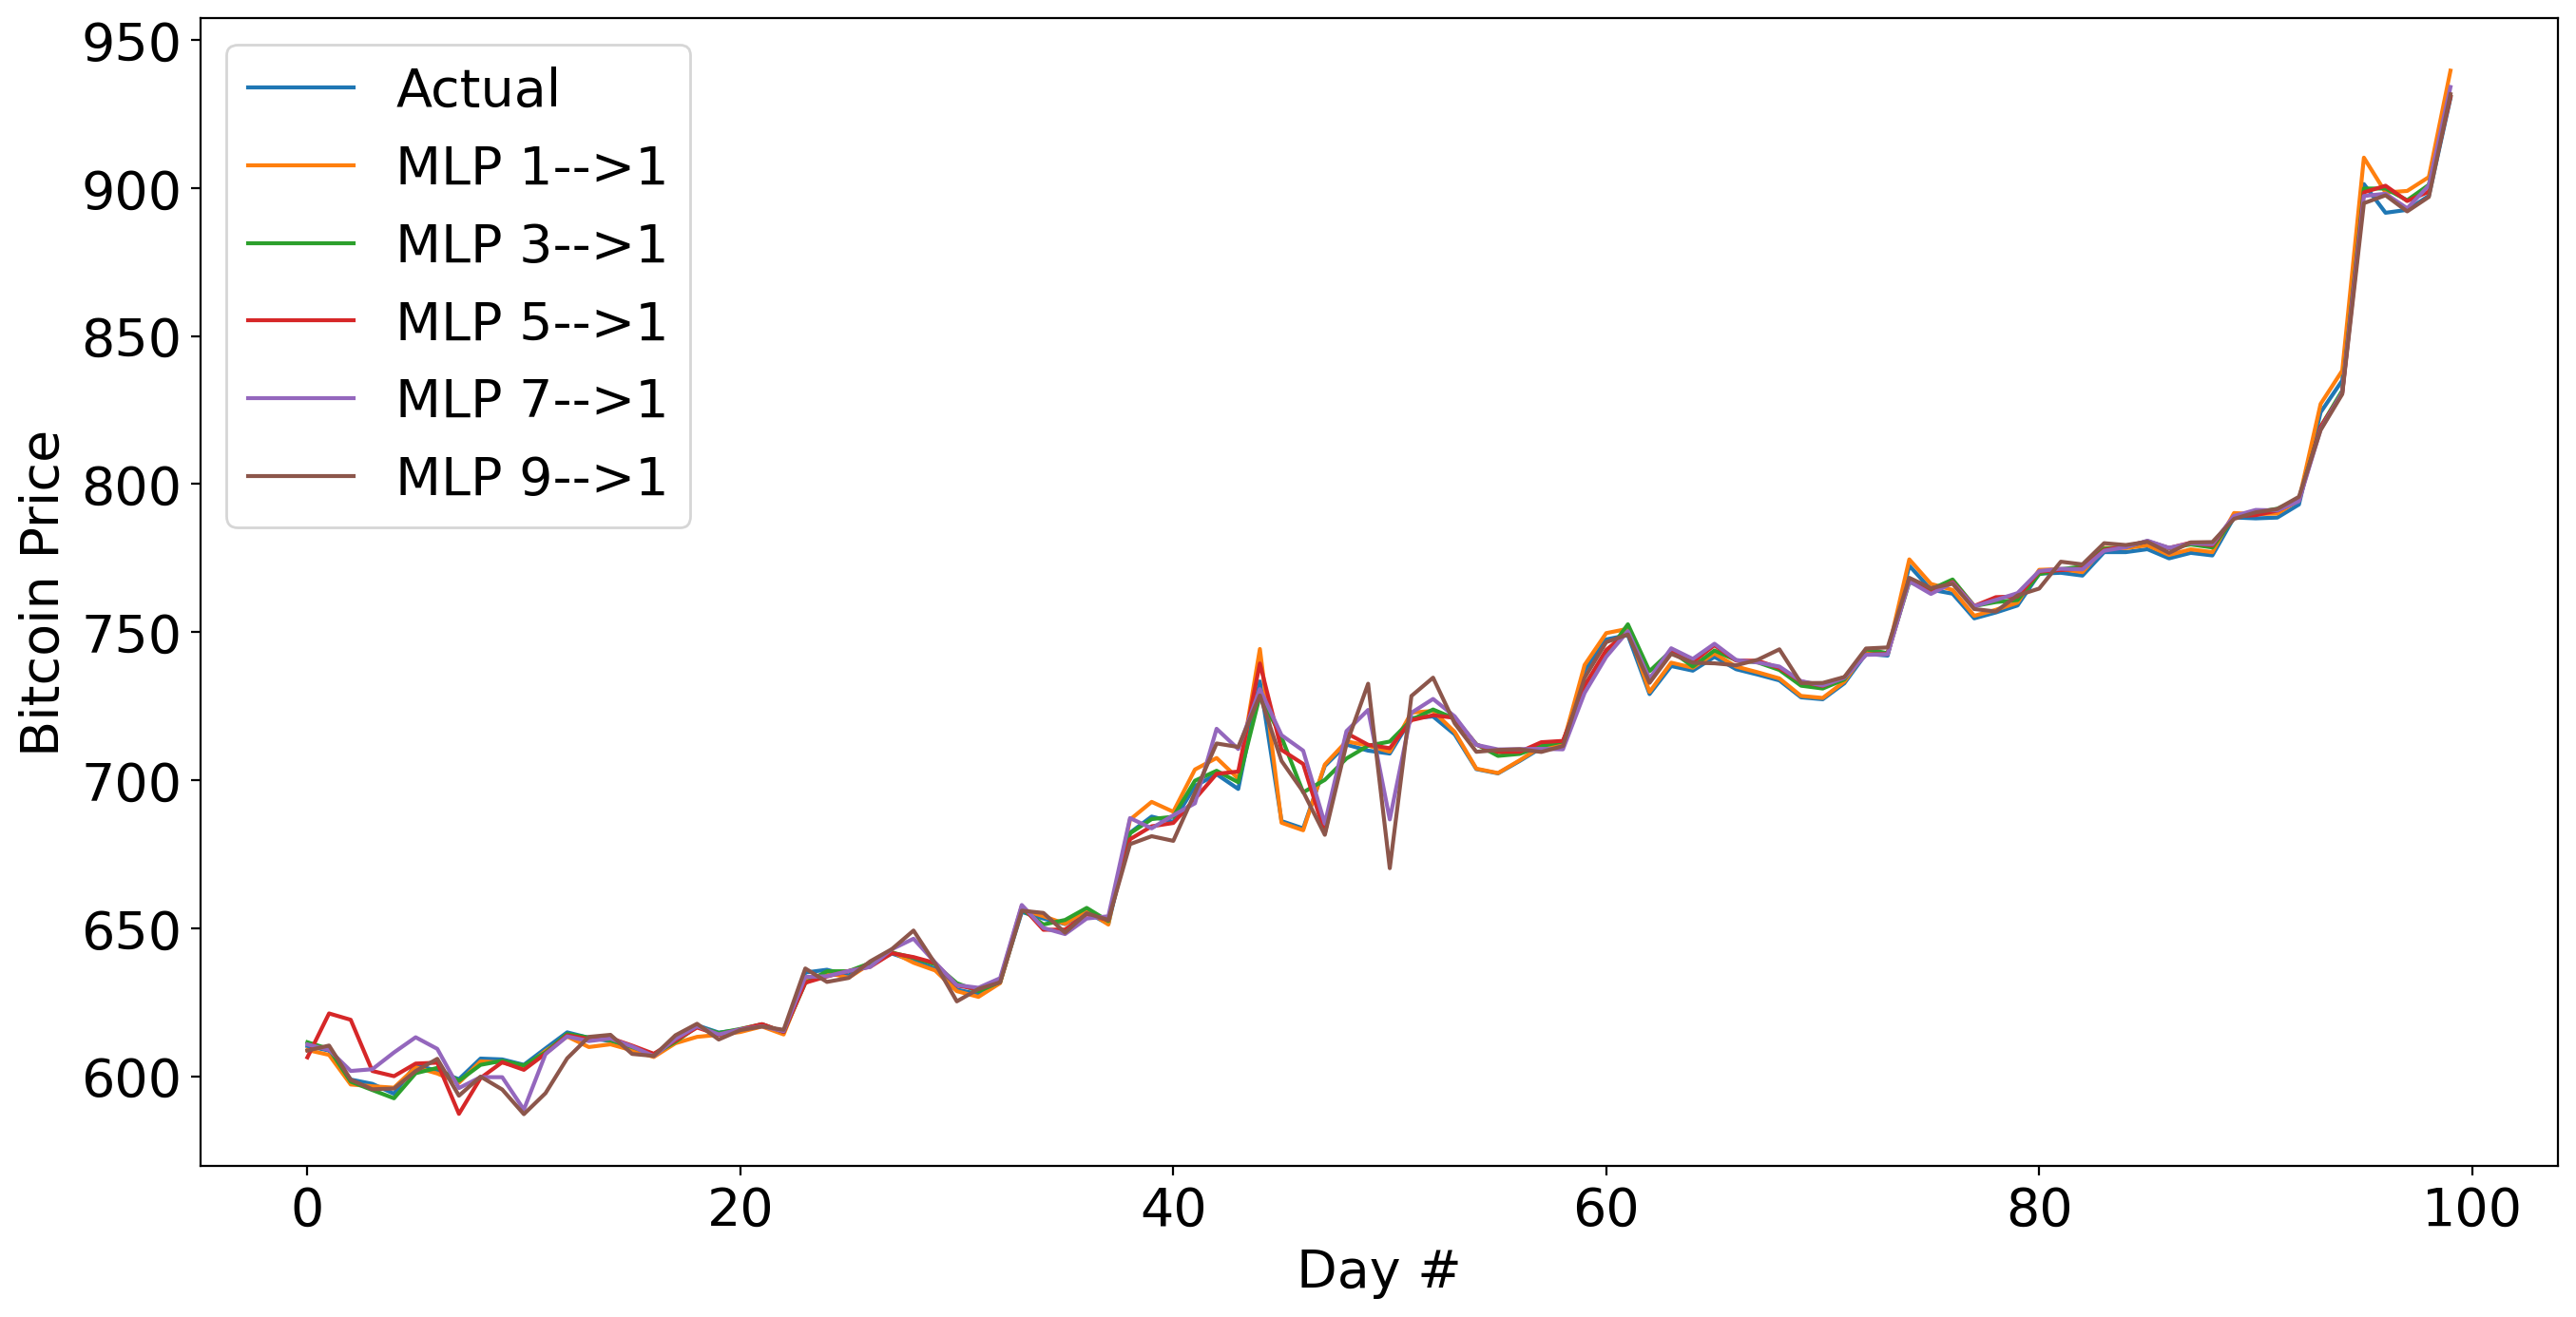
\includegraphics[width=8.1cm]{MLPBitcoinRoll}
		\caption{MLP rolling prediction of gold (left) and bitcoin (right) prices with various window sizes}
	\end{figure}
	
	\begin{figure}[h]
		\centering 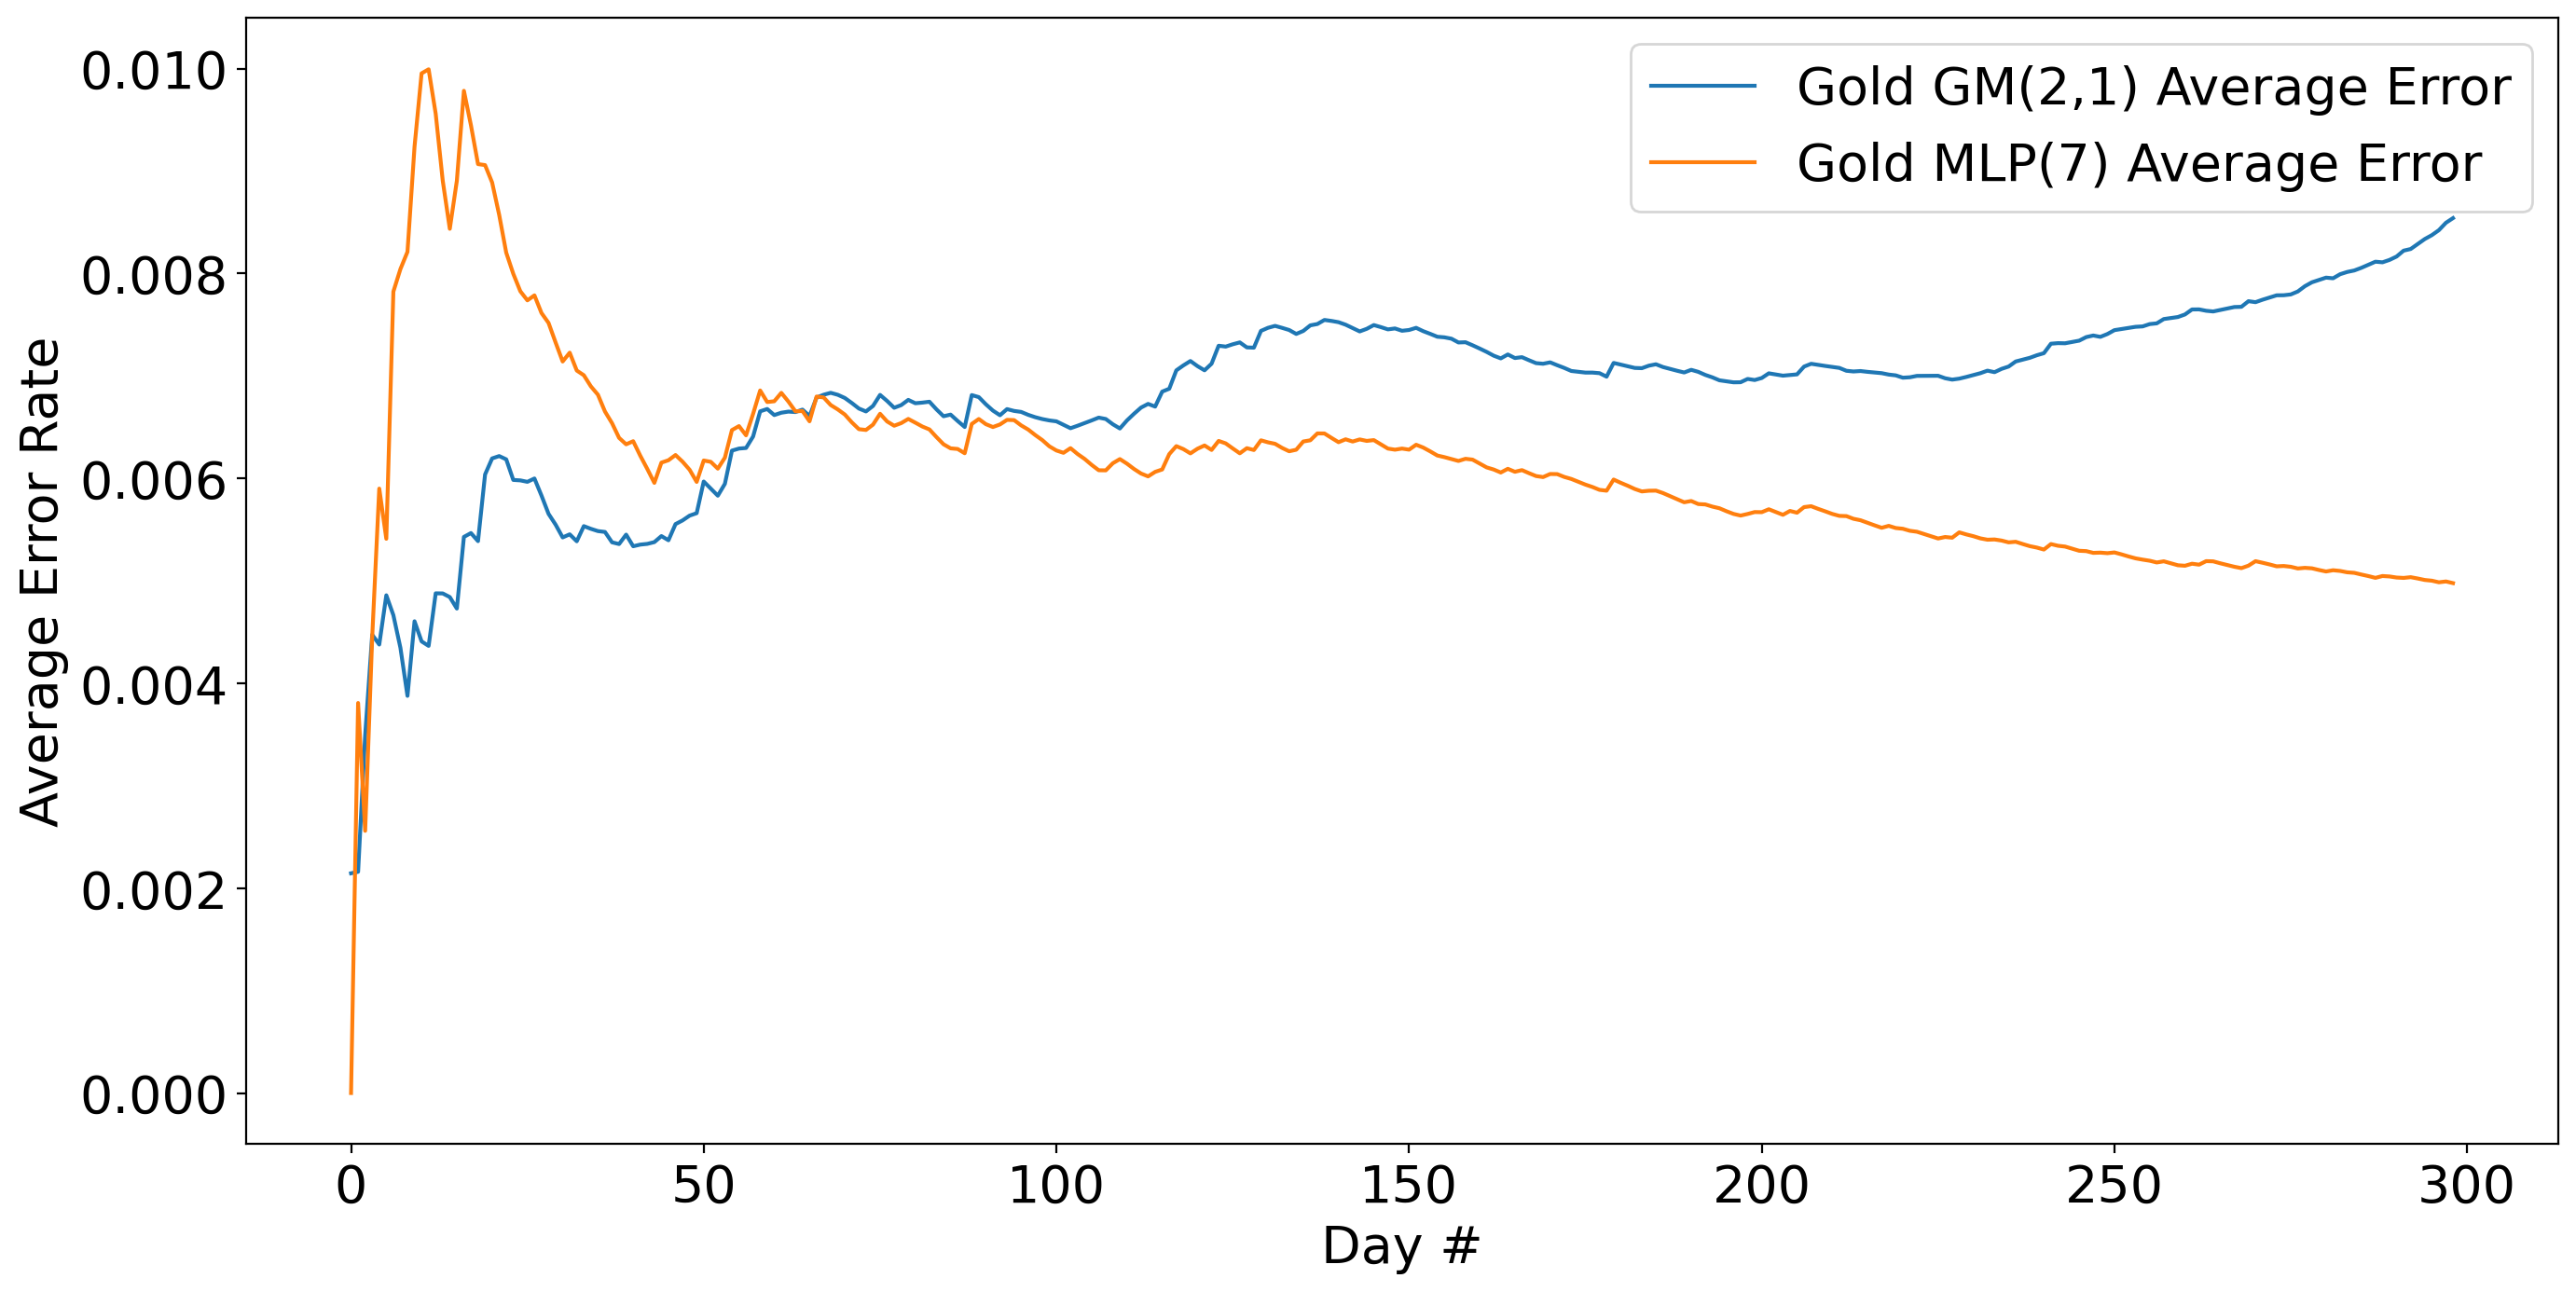
\includegraphics[width=8.1cm]{MLPGoldCompare}
		\centering 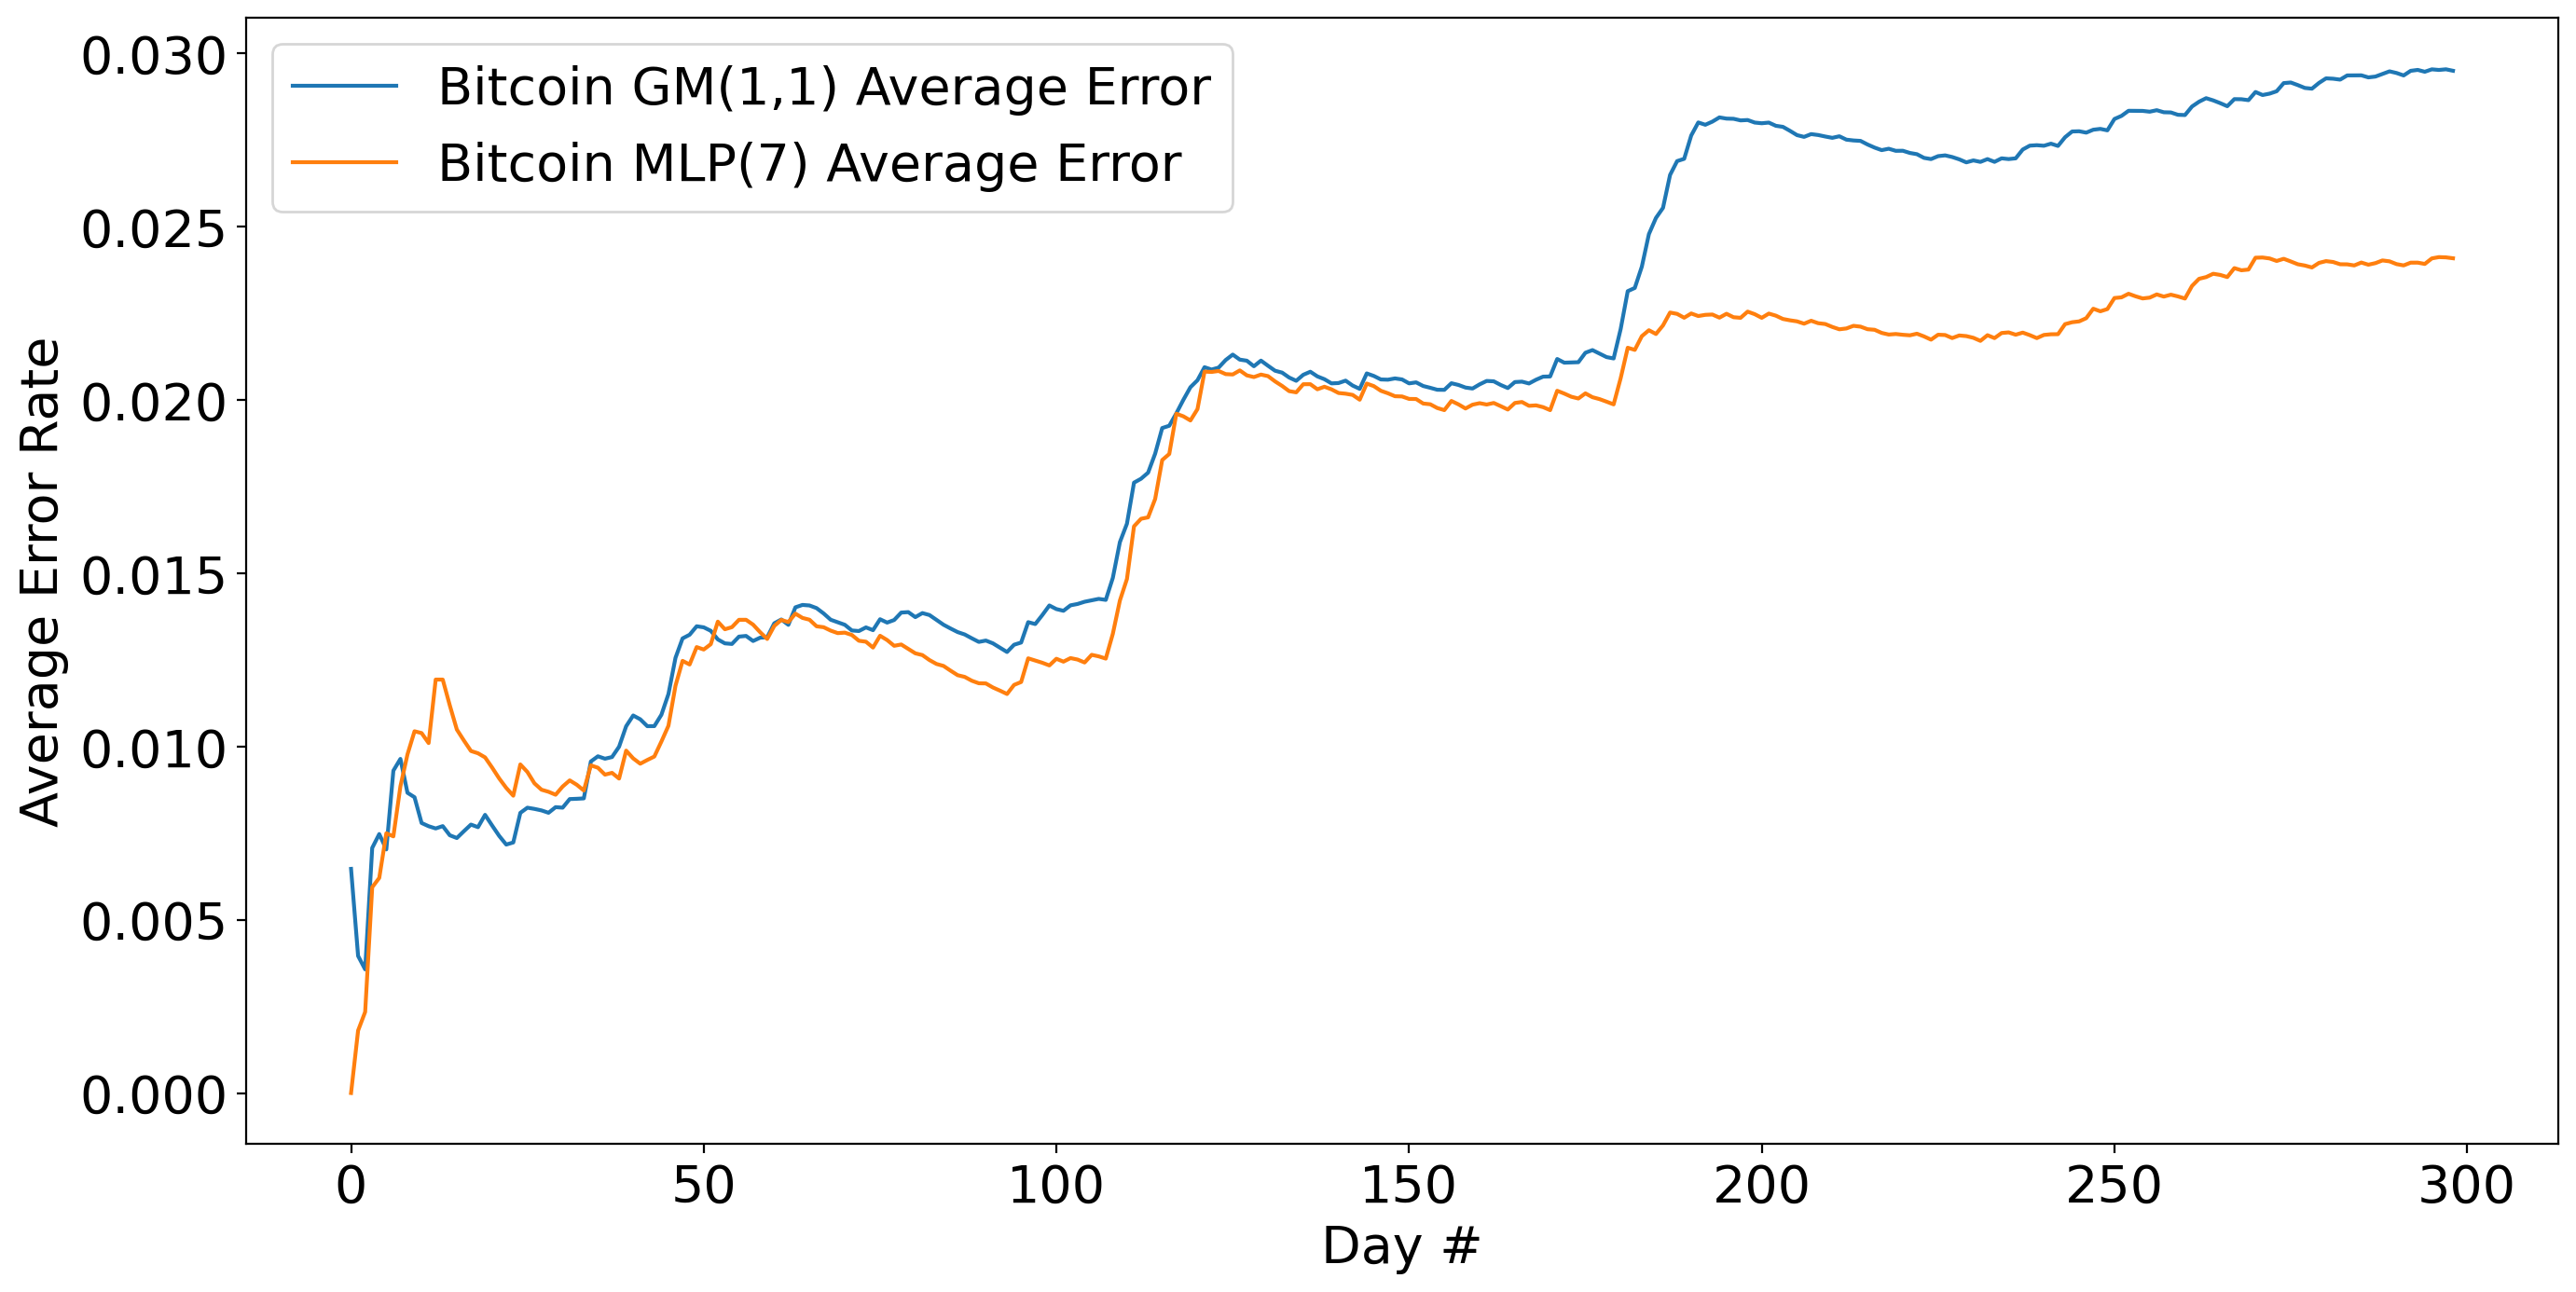
\includegraphics[width=8.1cm]{MLPBitcoinCompare}
		\caption{Comparation of GM and MLP moving average errors of gold (left) and bitcoin (right)}
	\end{figure}

	The window size of 7 is determined as the final choice to prevent overfitting while achieving relatively high accuracy. Since PDF instead of MWF is applied at the current stage of model selection, the model becomes more predictive with the increase of training actual data: the prediction accuracy of MLP eventually exceeds GM in the long run starting at roughly Day \#100 to \#200 (approximately 10\% of the total timespan). This suggests that neural networks are the ideal choice for making long-term predictions at the latter stage. 
	
	Once the hyperparameters are determined, the remaining task is to train the network. To zip the size and computation overhead, we turn to MWF-7 (data of last week as the window) and try to \textbf{predict next week's prices simultaneously} to verify its long-term prediction ability. 
	
	~\\
	
	\begin{figure}[h]
		\centering 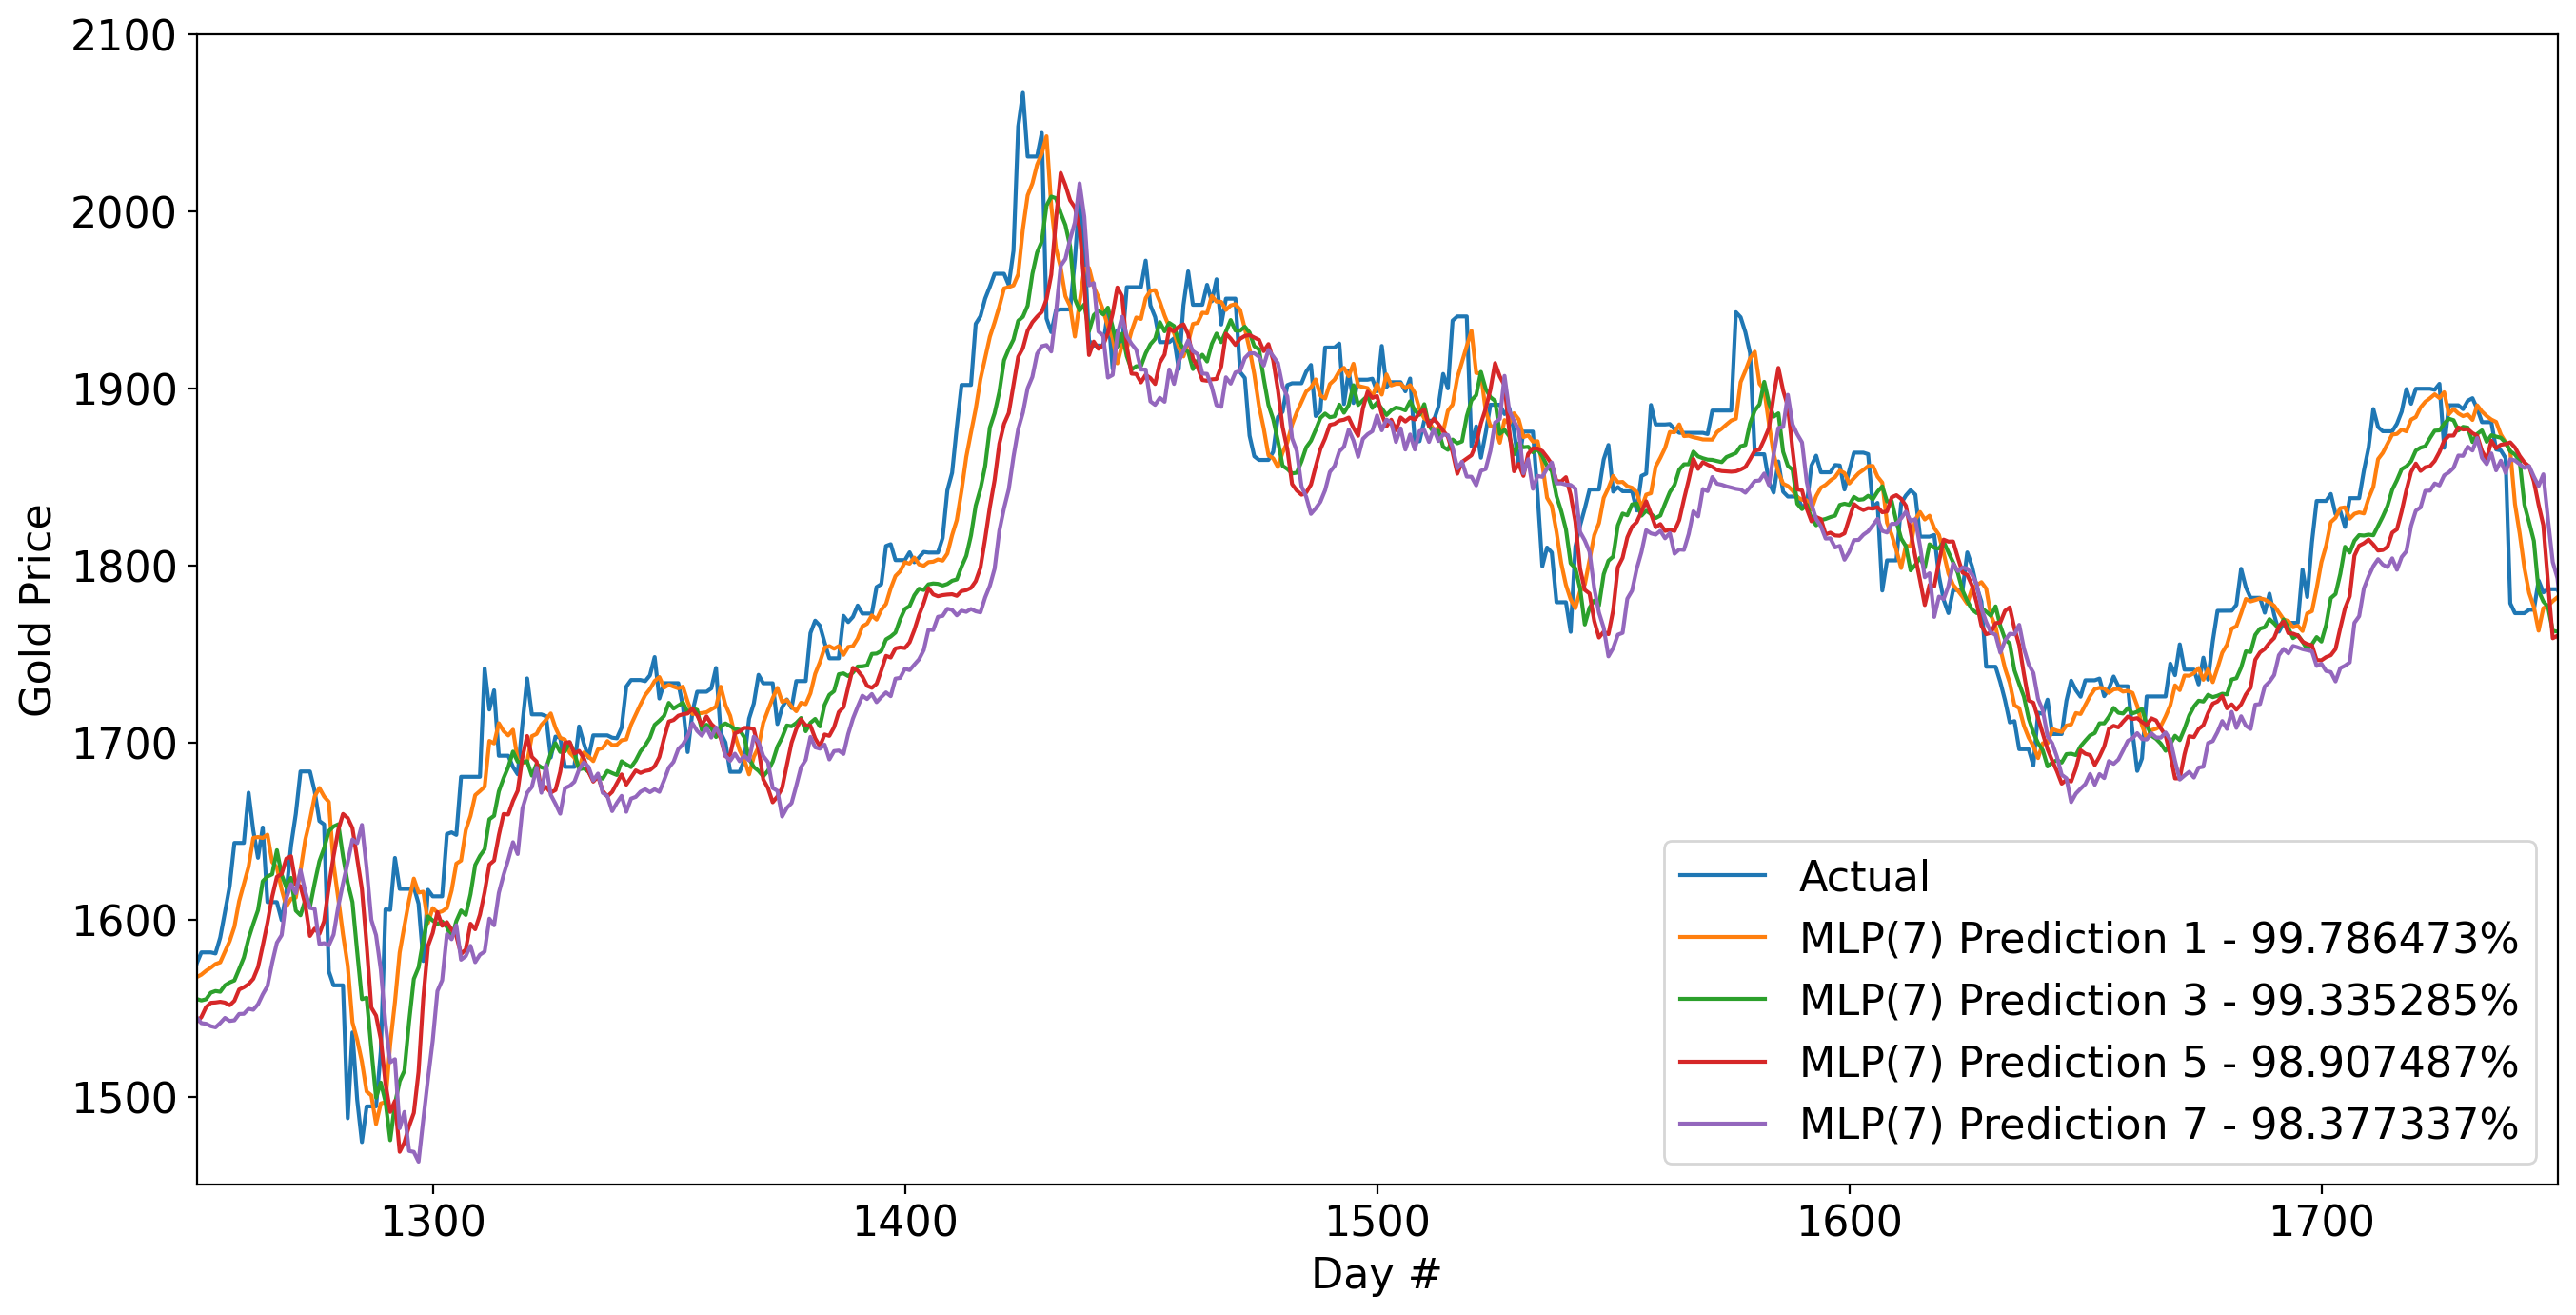
\includegraphics[width=8.1cm]{MLPGold}
		\centering 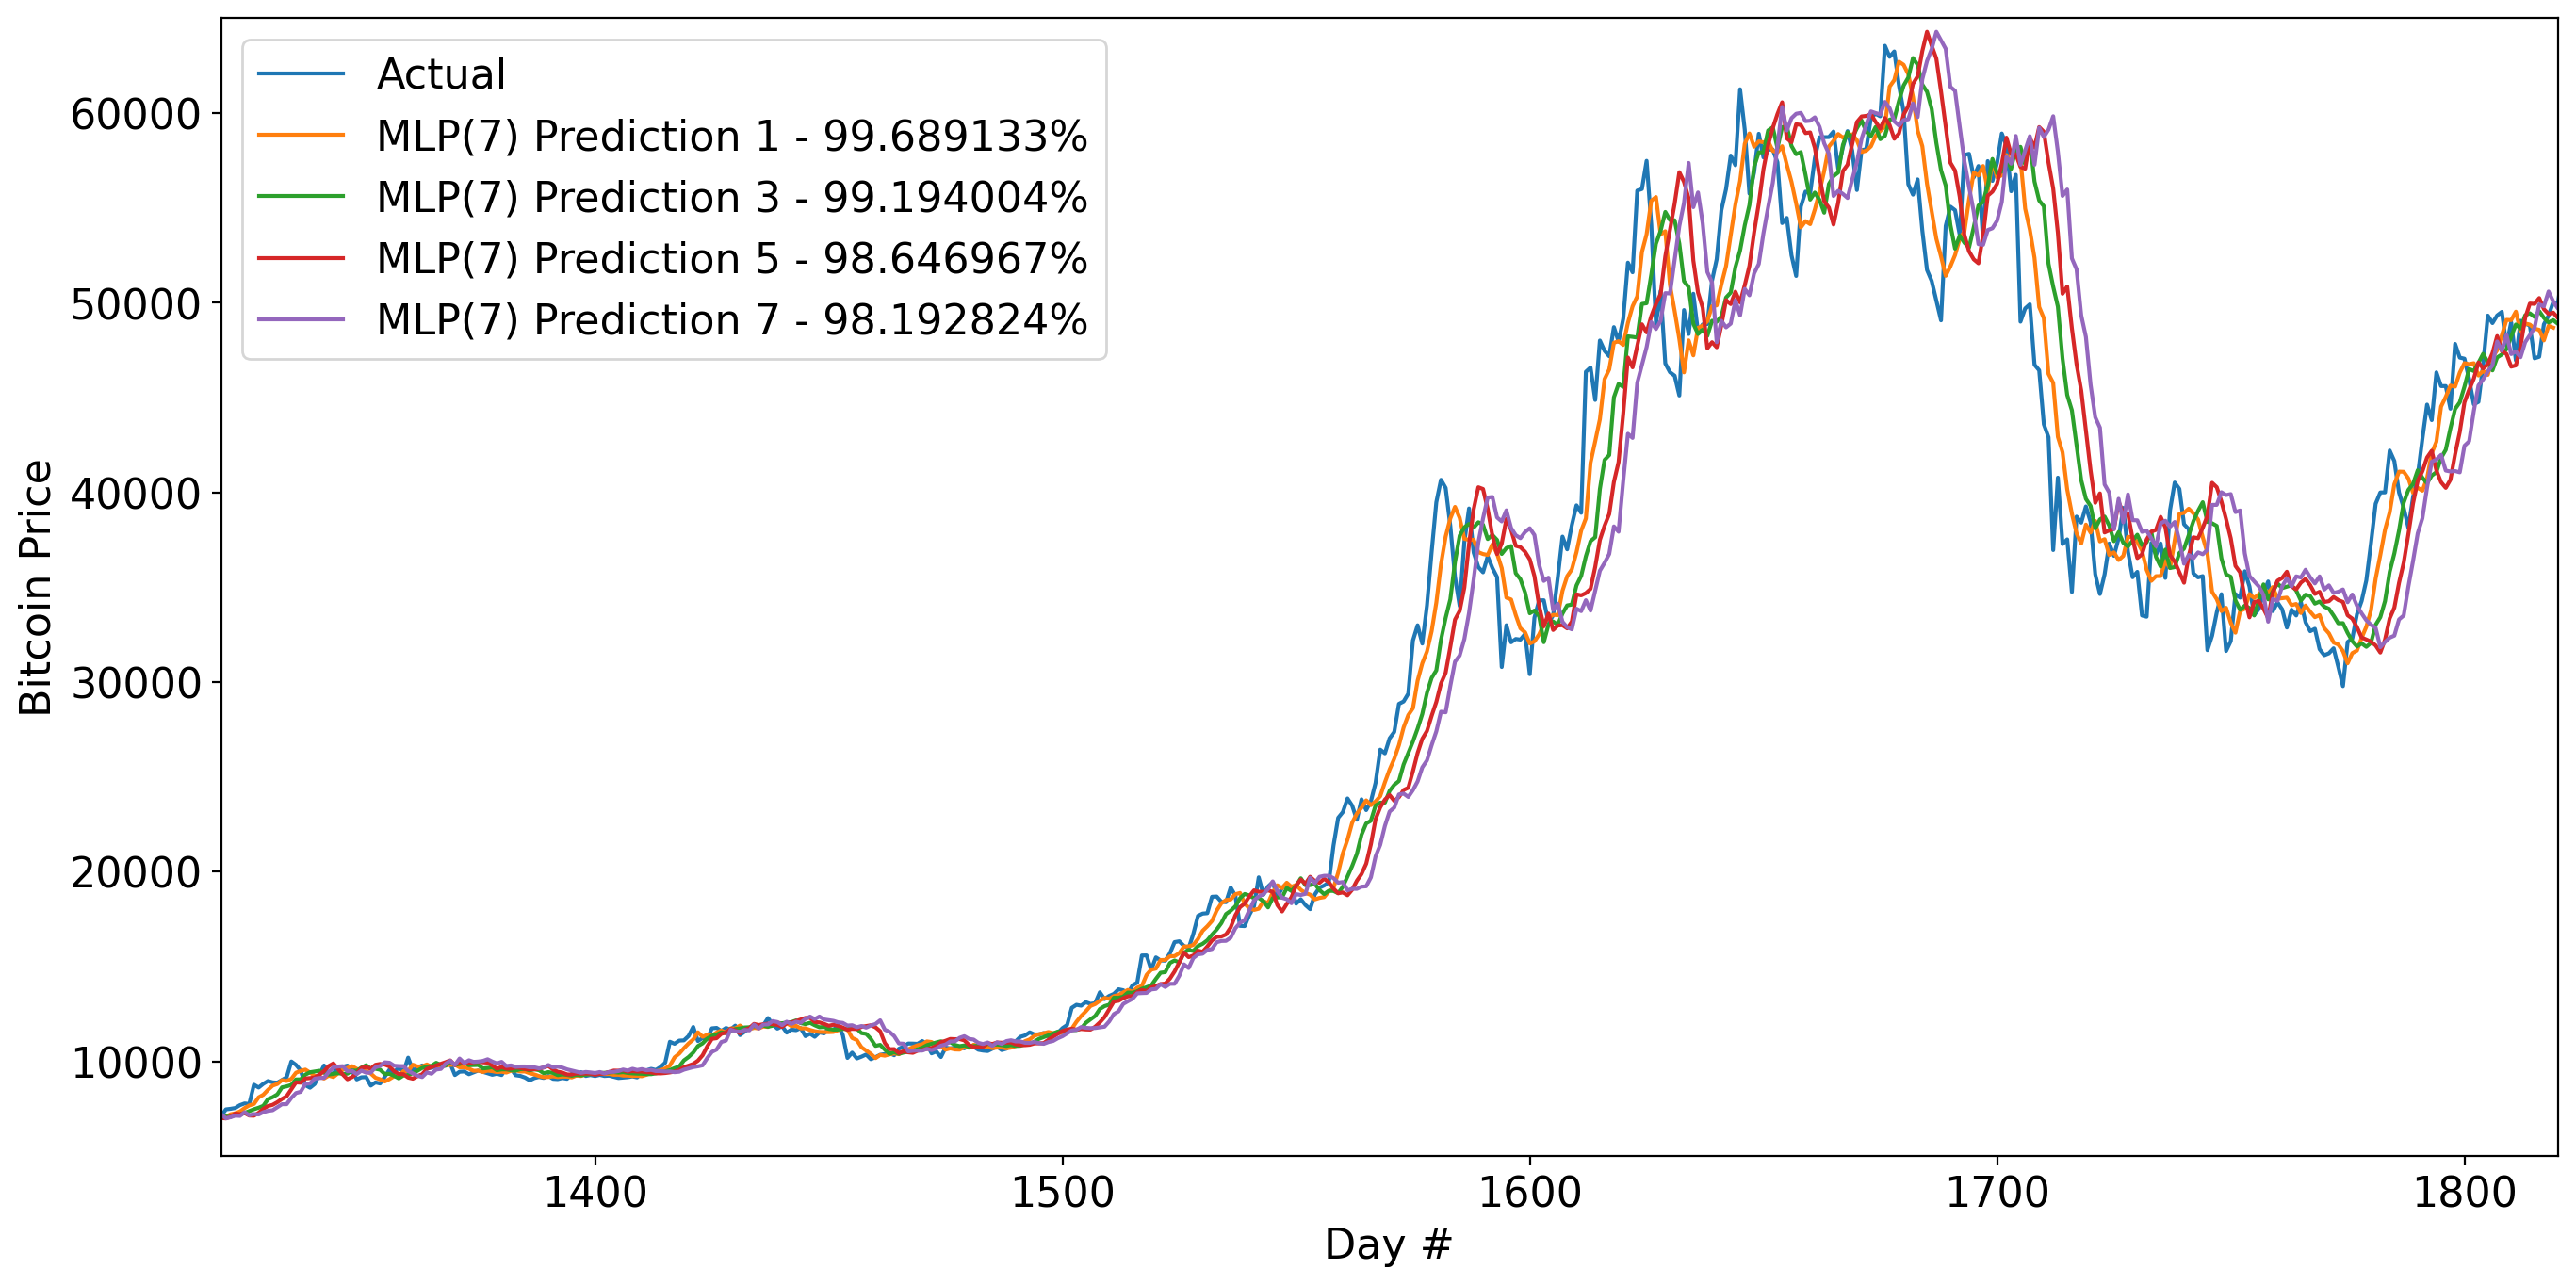
\includegraphics[width=8.2cm]{MLPBitcoin}
		\caption{MLP prediction of gold (left) and bitcoin (right) prices: 7 days in, 7 days out}
	\end{figure}
	
	\begin{figure}[h]
		\centering 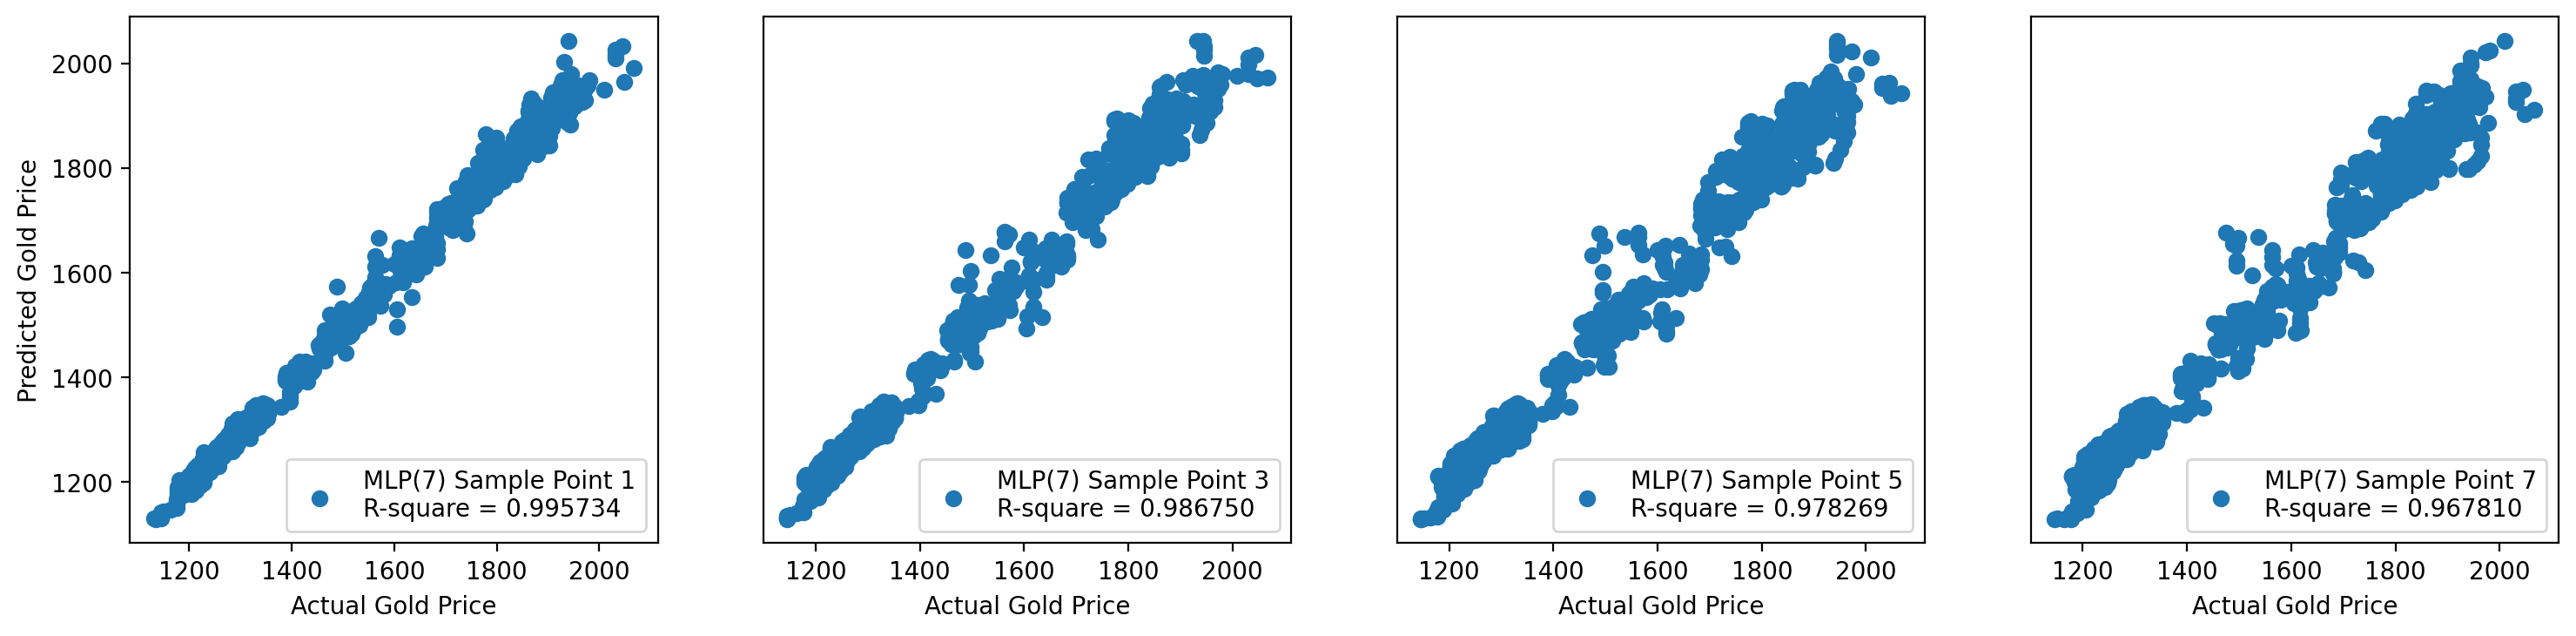
\includegraphics[width=16cm]{MLPGoldCorr}
		\centering 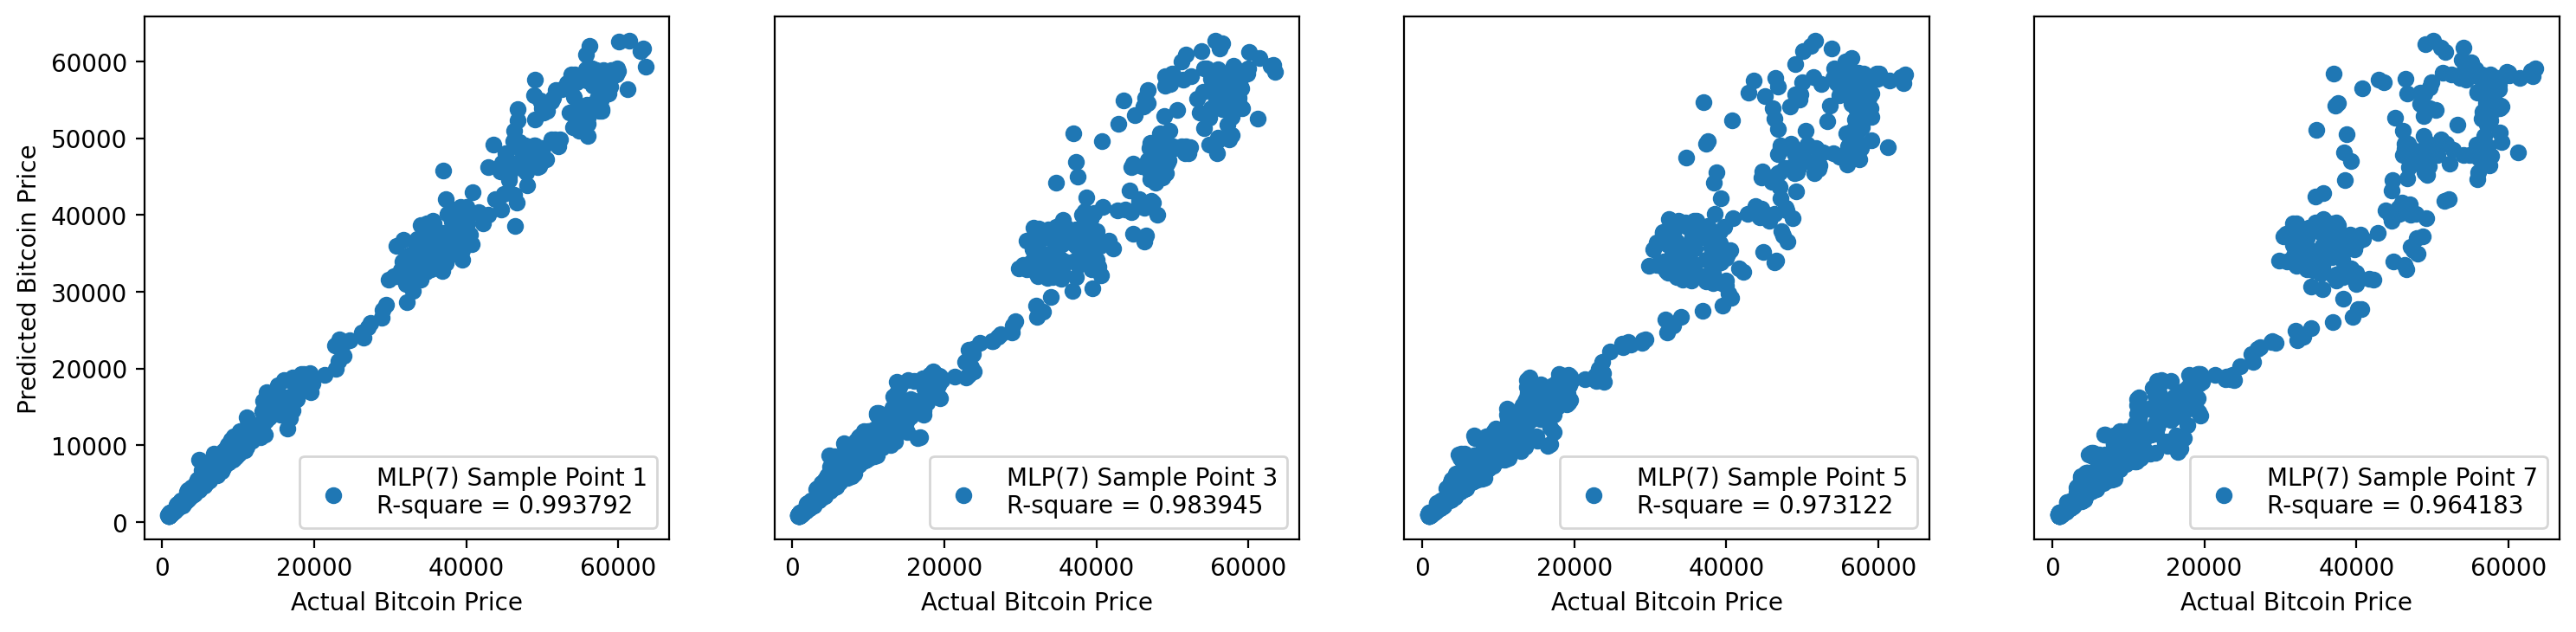
\includegraphics[width=16.1cm]{MLPBitcoinCorr}
		\caption{Correlation between MLP predicted and actual prices of gold (top) and bitcoin (bottom)}
	\end{figure}
	
	These figures carry some interesting traits. As the prediction period increases, both models experience a time lag again -- possibly due to the switch from PDF to MWF-7. Yet they are showing opposite trends of deviation: in the line chart, the gold price deviates downward as time goes by, while the bitcoin price deviates upward; the scattering points cluster to center for gold prices, while they aggregate towards two ends like a dumbbell for bitcoin prices. It reveals that \textbf{MLP is making safe choices} -- the gold price fluctuates around a \textit{center} value, while the bitcoin price is relatively \textit{low} before 2021 but experiences a sharp \textit{rise} afterwards. Such patterns can probably give us insights into the differences in characteristics and trends of the two assets' prices. 
	
	\textbf{SVM} plays a vital role in the non-linear regression and classification problems of small samples, presenting another choice of data mining and prediction. For this model, we perform \textbf{data dimension rising} with 3 combinations of taking the $x^{th}$-order difference (diff-$x$), average price over the past $x$ days (mean-$x$), and standard deviation over the last $x$ days (std-$x$). 
	
	\begin{center}
		\begin{tabular}{cl}
			\toprule
			Position & Combination \\ \midrule
			top & data, diff-1, mean-7, std-7 \\
			middle & data, diff-1, mean-15, std-15 \\
			bottom & data, diff-1, diff-2, mean-7, mean-15, std-7, std-15 \\
			\bottomrule
		\end{tabular}
	\end{center}
	
	\begin{figure}[h]
		\centering 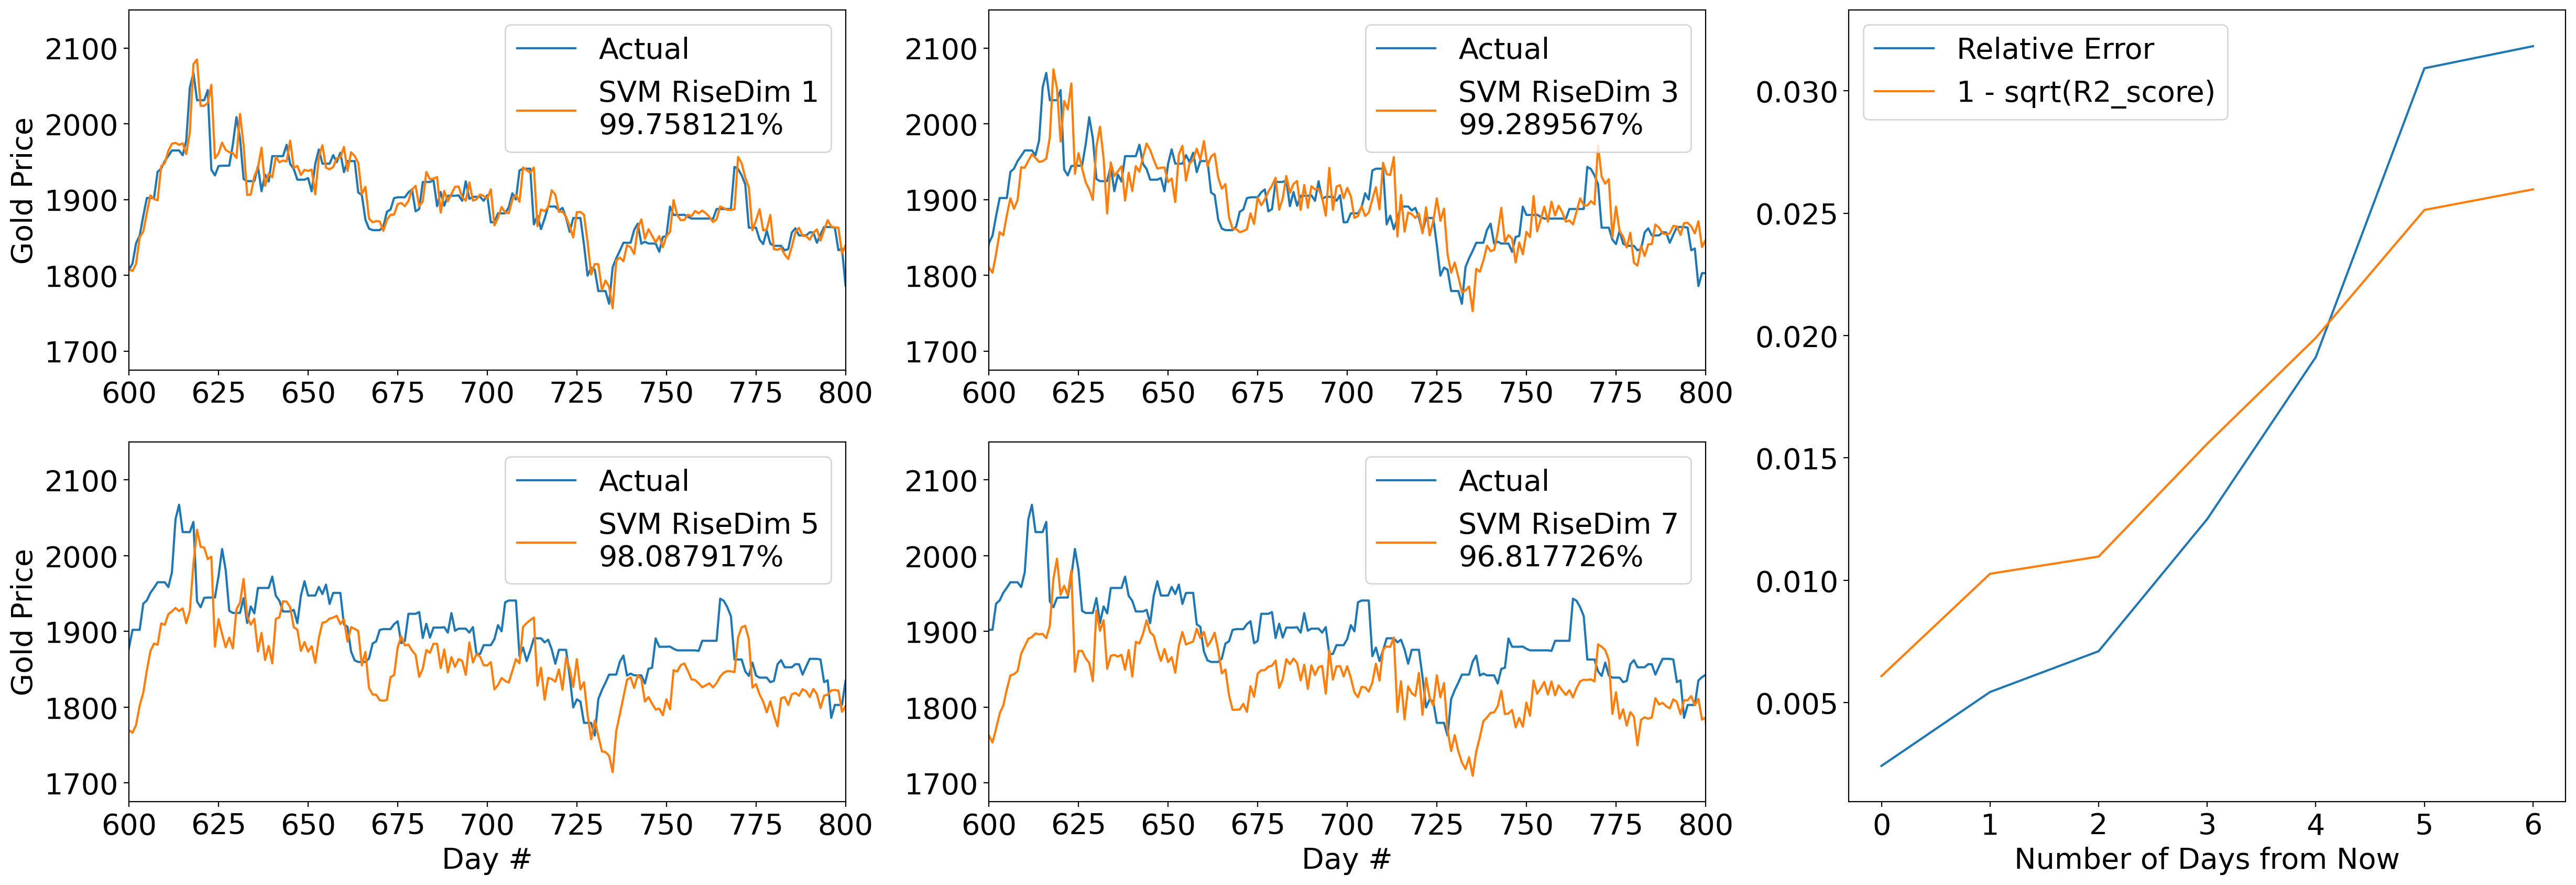
\includegraphics[width=15.6cm]{SVMGold1AA}
		\centering 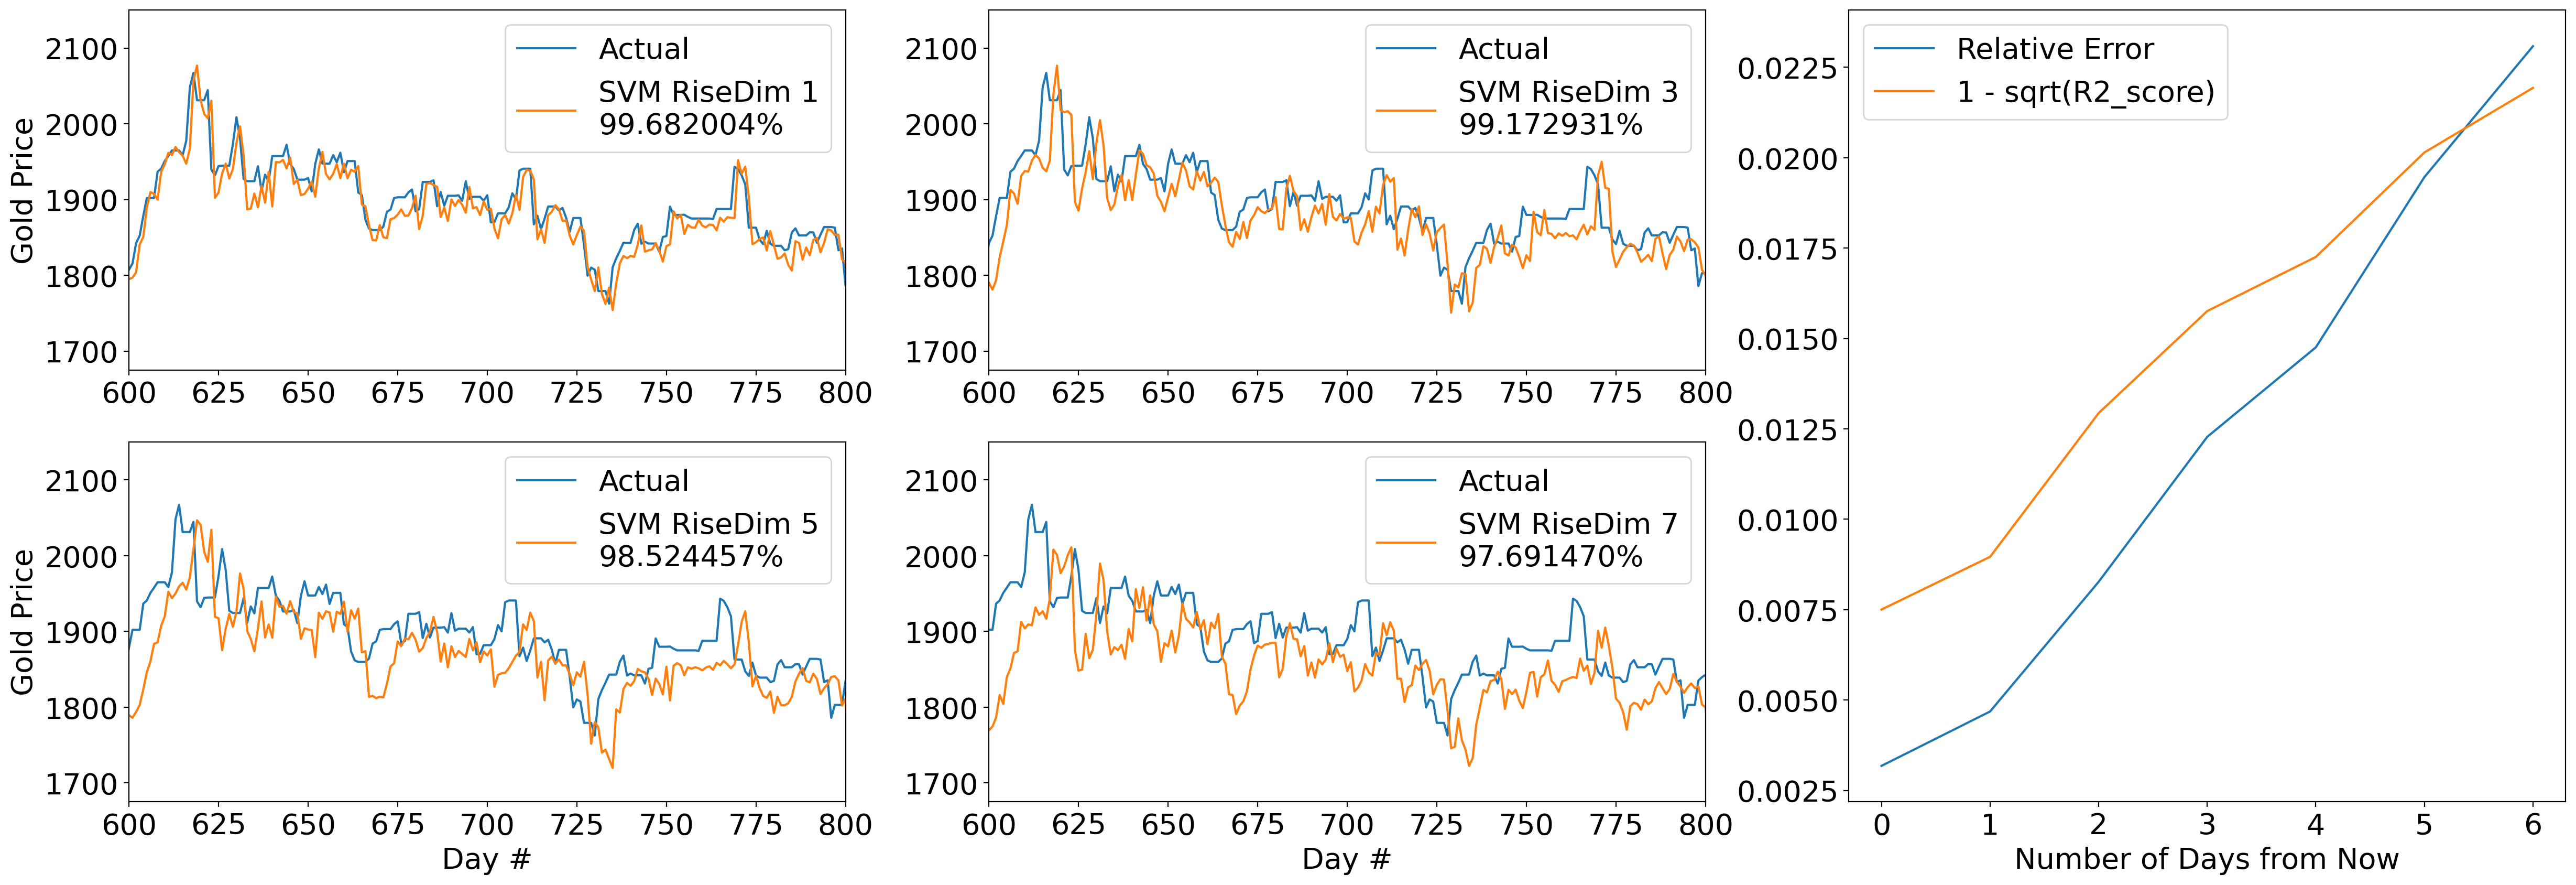
\includegraphics[width=15.6cm]{SVMGold1BB}
		\centering 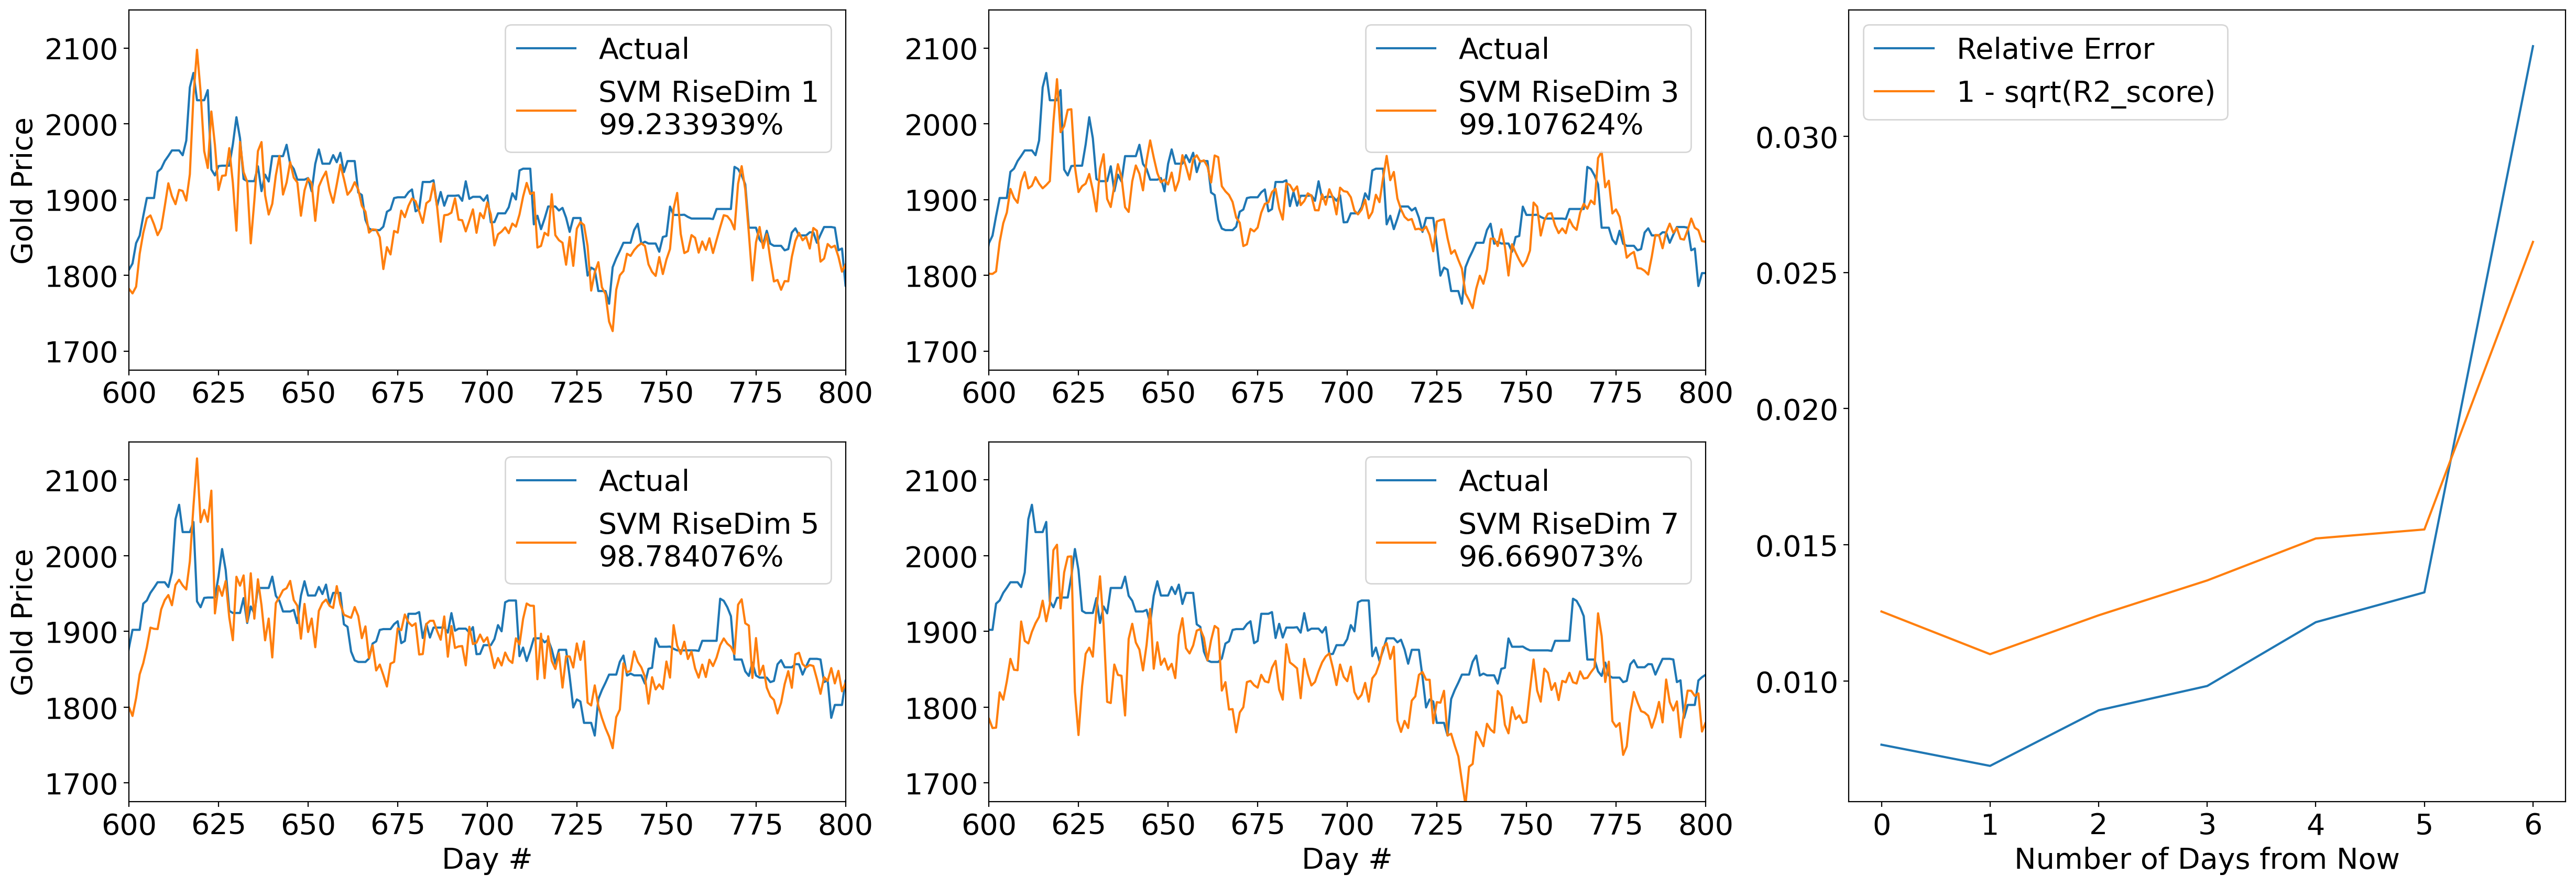
\includegraphics[width=15.6cm]{SVMGold12ABAB}
		\caption{MLP prediction of gold prices (Predictions within 1, 3, 5, 7 days drawn)}
	\end{figure}
	
	The accuracy is satisfying, despite that the training epochs of SVM take relatively longer than MLP. As we predict further into the future, the charts show that both time lag and negative error accumulates -- yet the middle combination is most resilient to such deviation. This gives us two insights of choosing dimension-rising strategies: (1) to prefer long-term conclusive criteria over short-term ones and (2) to limit the total number and complexity of criteria. \textit{Also note that the bitcoin price series fails to train SVM, probably due to uncertainty from overly strong fluctuation. }
	
	\subsection{Combining for a General Prediction (GM+MLP)}
	\label{sec:3.4}
	
	To proceed into the next stage of designing an investment strategy, we develop a method to combine predictions both in short term (based on few data) and in long term (based on more data). As explained in the former sections, ARIMA must be trained on large amounts of data, experiences a serious time lag, and is vulnerable to overfitting; GM(1,1) is predictive of the general trend and GM(2,2) is more sensitive to details, but both require a careful selection between PDF and MWF-$x$, and the predicted values blow up rapidly as the model looks into future; MLP outweighs GM in the long run, but tends to make safe guesses to fit the existing trend, and SVM takes much longer to train than MLP and is occasionally unstable. 
	
	To apply our algorithm of CAPM discussed in later sessions, it is necessary to predict asset prices 1, 7, and 15 days from now. Taking the advantages and drawbacks of various models into consideration, we make no predictions in the first 7 days, apply \textbf{GM(1,1) PDF to the former 10\%} of data, and apply \textbf{MLP MWF-15 to the latter 90\%} with data dimensions raised with \textbf{diff-1 and std-15} operands. The design philosophy is to make rough predictions and accumulate real-life information before diving into the details like price fluctuations on a daily basis. \textit{Note that predictions are accepted based on either high correlation (high $R^2$-score) or low error rate. }
	
	\begin{center}
		\begin{tabular}{l|rccr}
			\toprule
			& Gold $R^2$ & Gold Error & Bitcoin $R^2$ & Bitcoin Error \\ \midrule
			GM Pred 1 day & \sout{0.238762} & 3.325490\% & 0.904871 & 3.905270\% \\
			GM Pred 7 days & \sout{-0.498381} & 4.559821\% & 0.883330 & 4.820433\% \\
			GM Pred 15 days & \sout{-2.277892} & 5.825080\% & 0.815899 & 6.416537\% \\
			MLP Pred 1 day & 0.991459 & 1.033804\% & 0.992472 & 4.642692\% \\
			MLP Pred 7 days & 0.963941 & 2.137616\% & 0.958148 & \sout{12.234482\%} \\
			MLP Pred 15 days & 0.927715 & 3.173871\% & 0.906519 & \sout{19.223700\%} \\
			\bottomrule
		\end{tabular}
	\end{center}
	
	\begin{figure}[h]
		\label {fig:11}
		\centering 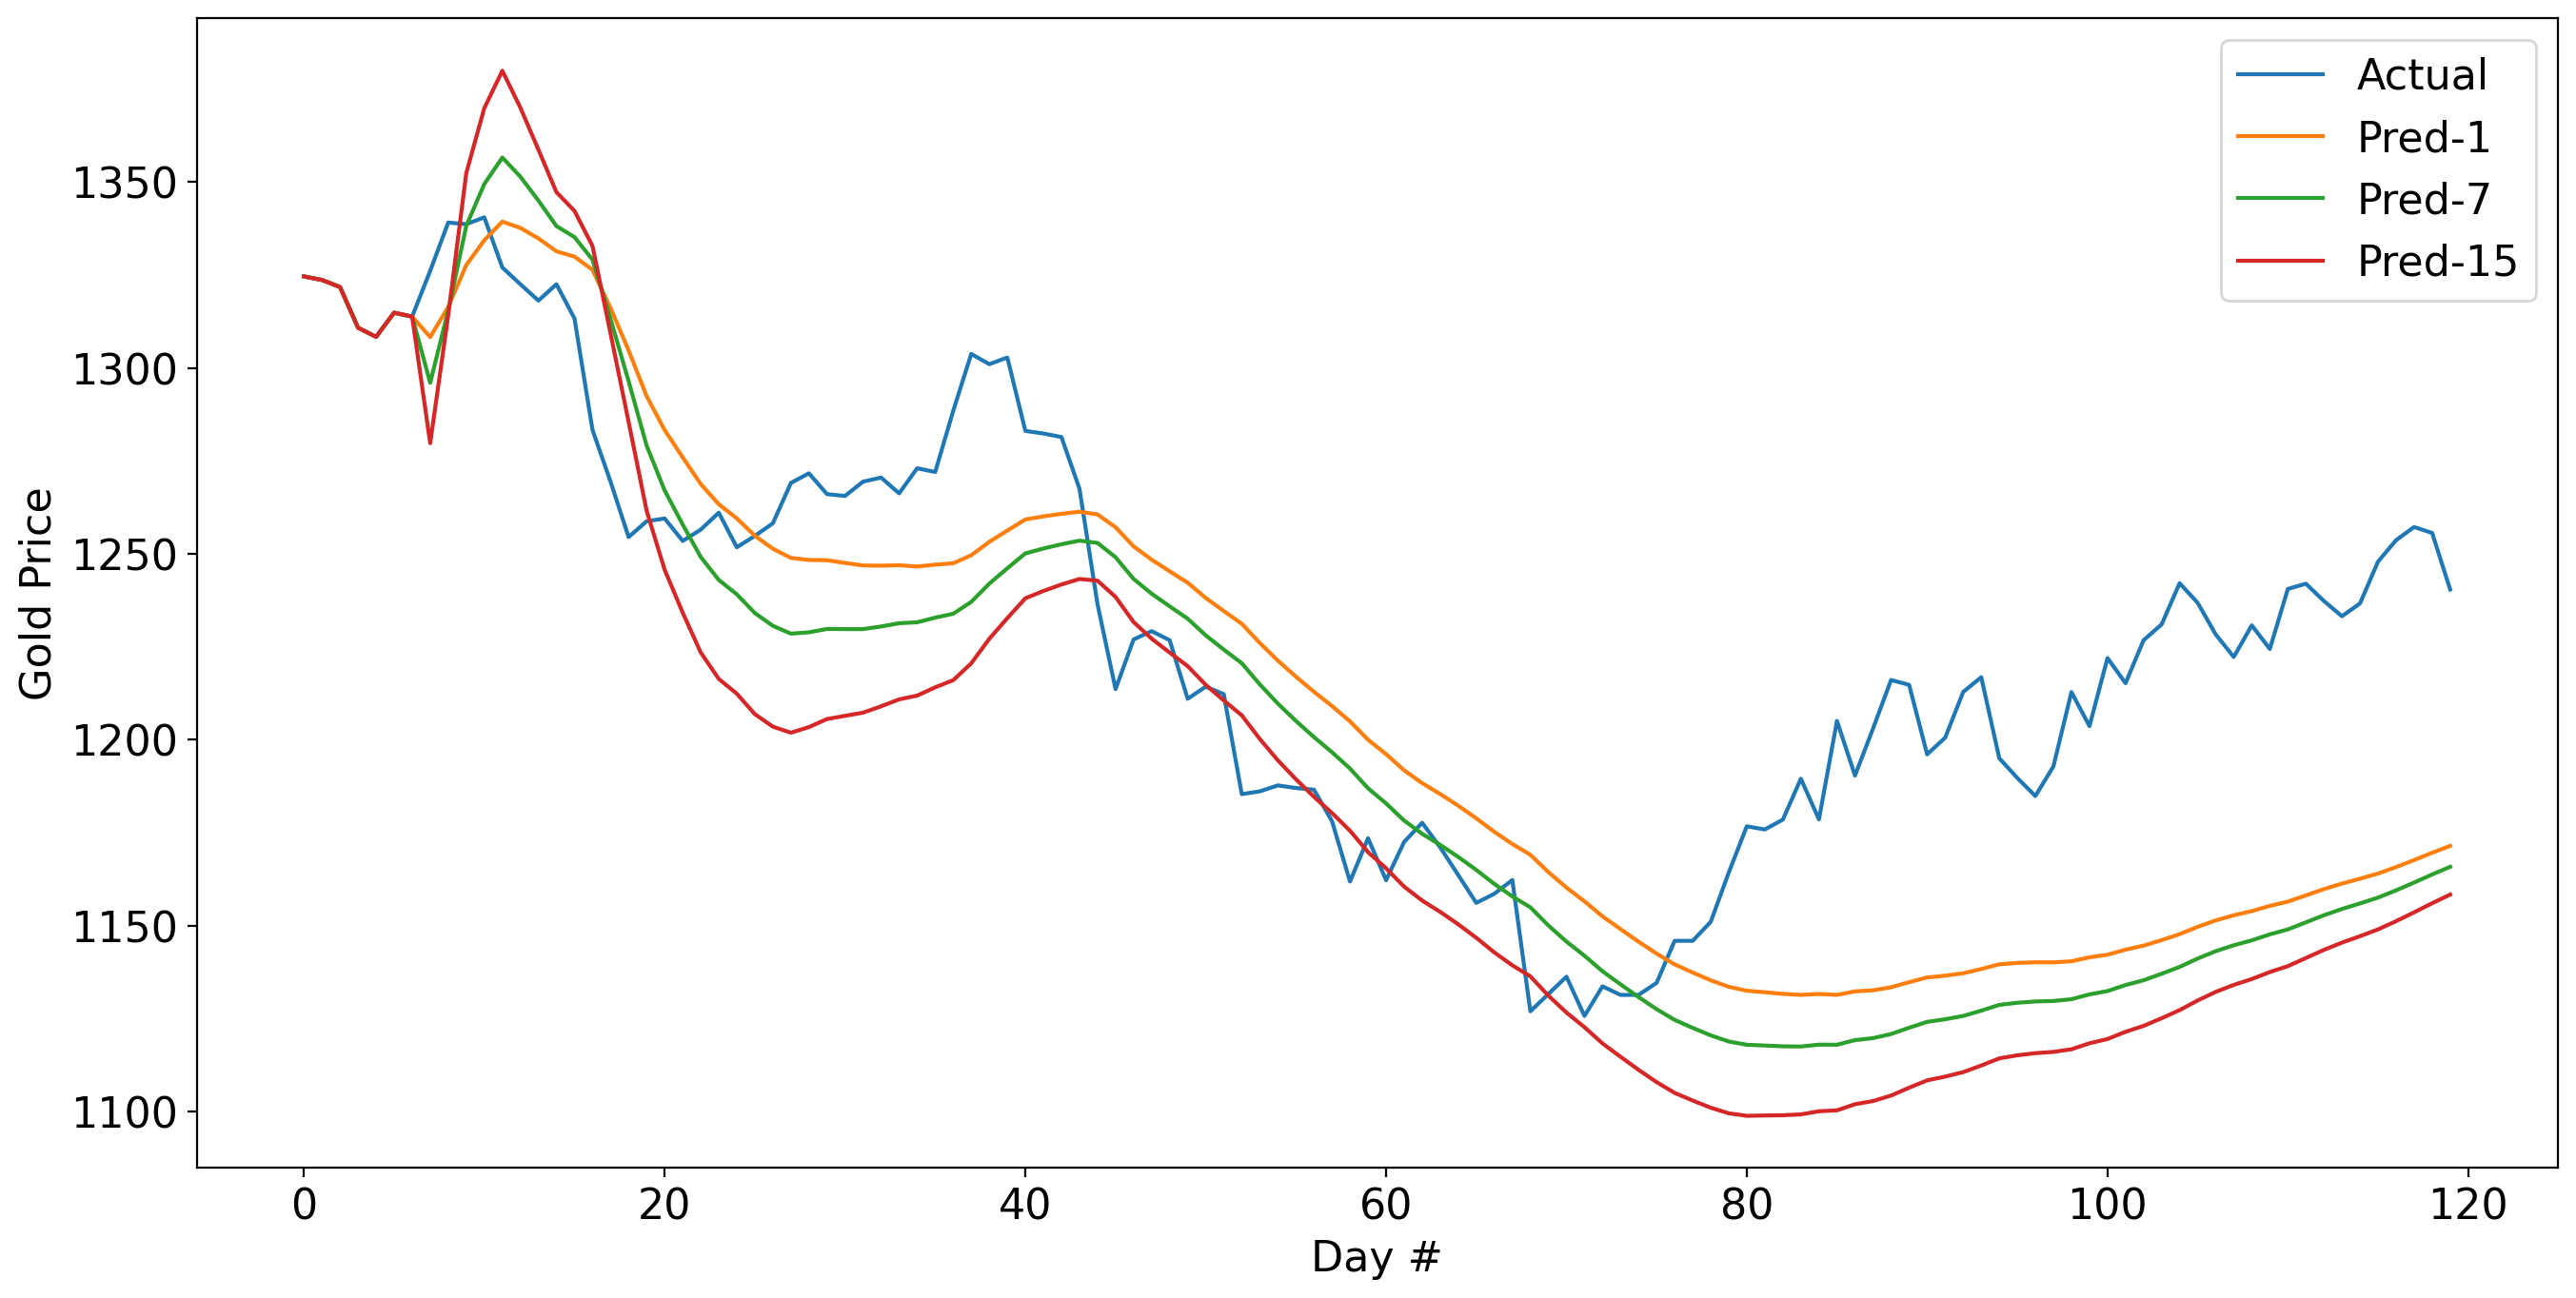
\includegraphics[width=8cm]{FinalGoldS}
		\centering 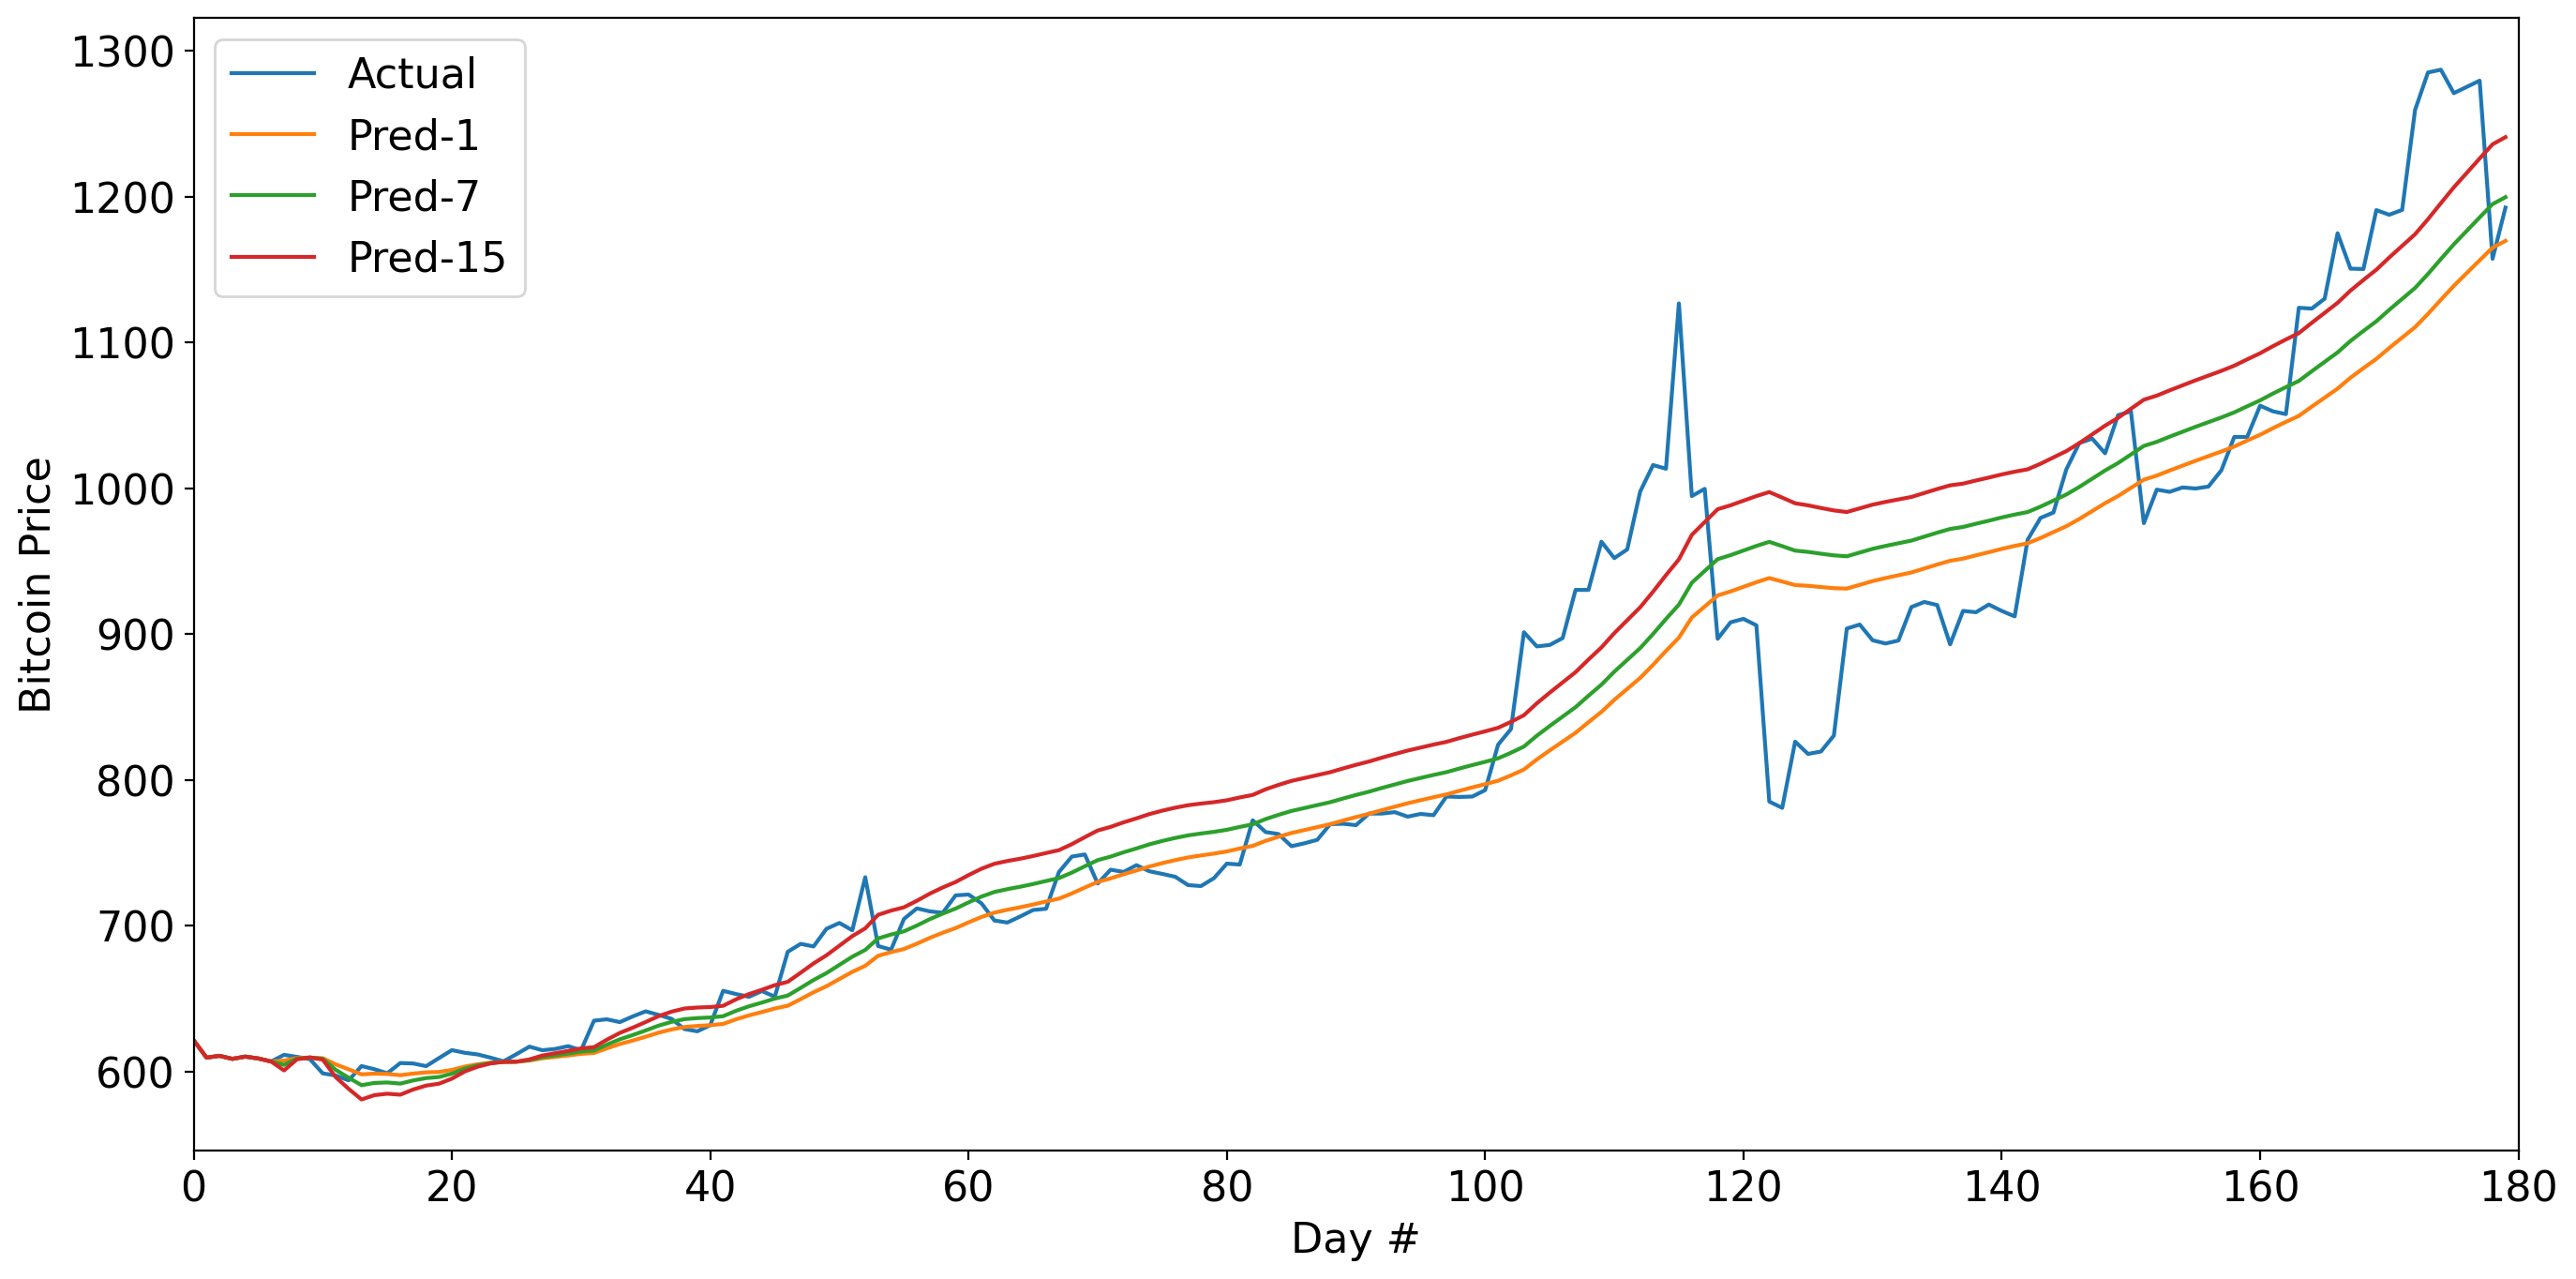
\includegraphics[width=8.1cm]{FinalBitcoinS}
		\caption{Short-term prediction of gold (left) and bitcoin (right) prices using \textbf{GM(1,1) PDF}}
	\end{figure}
	
	\begin{figure}[h]
		\centering 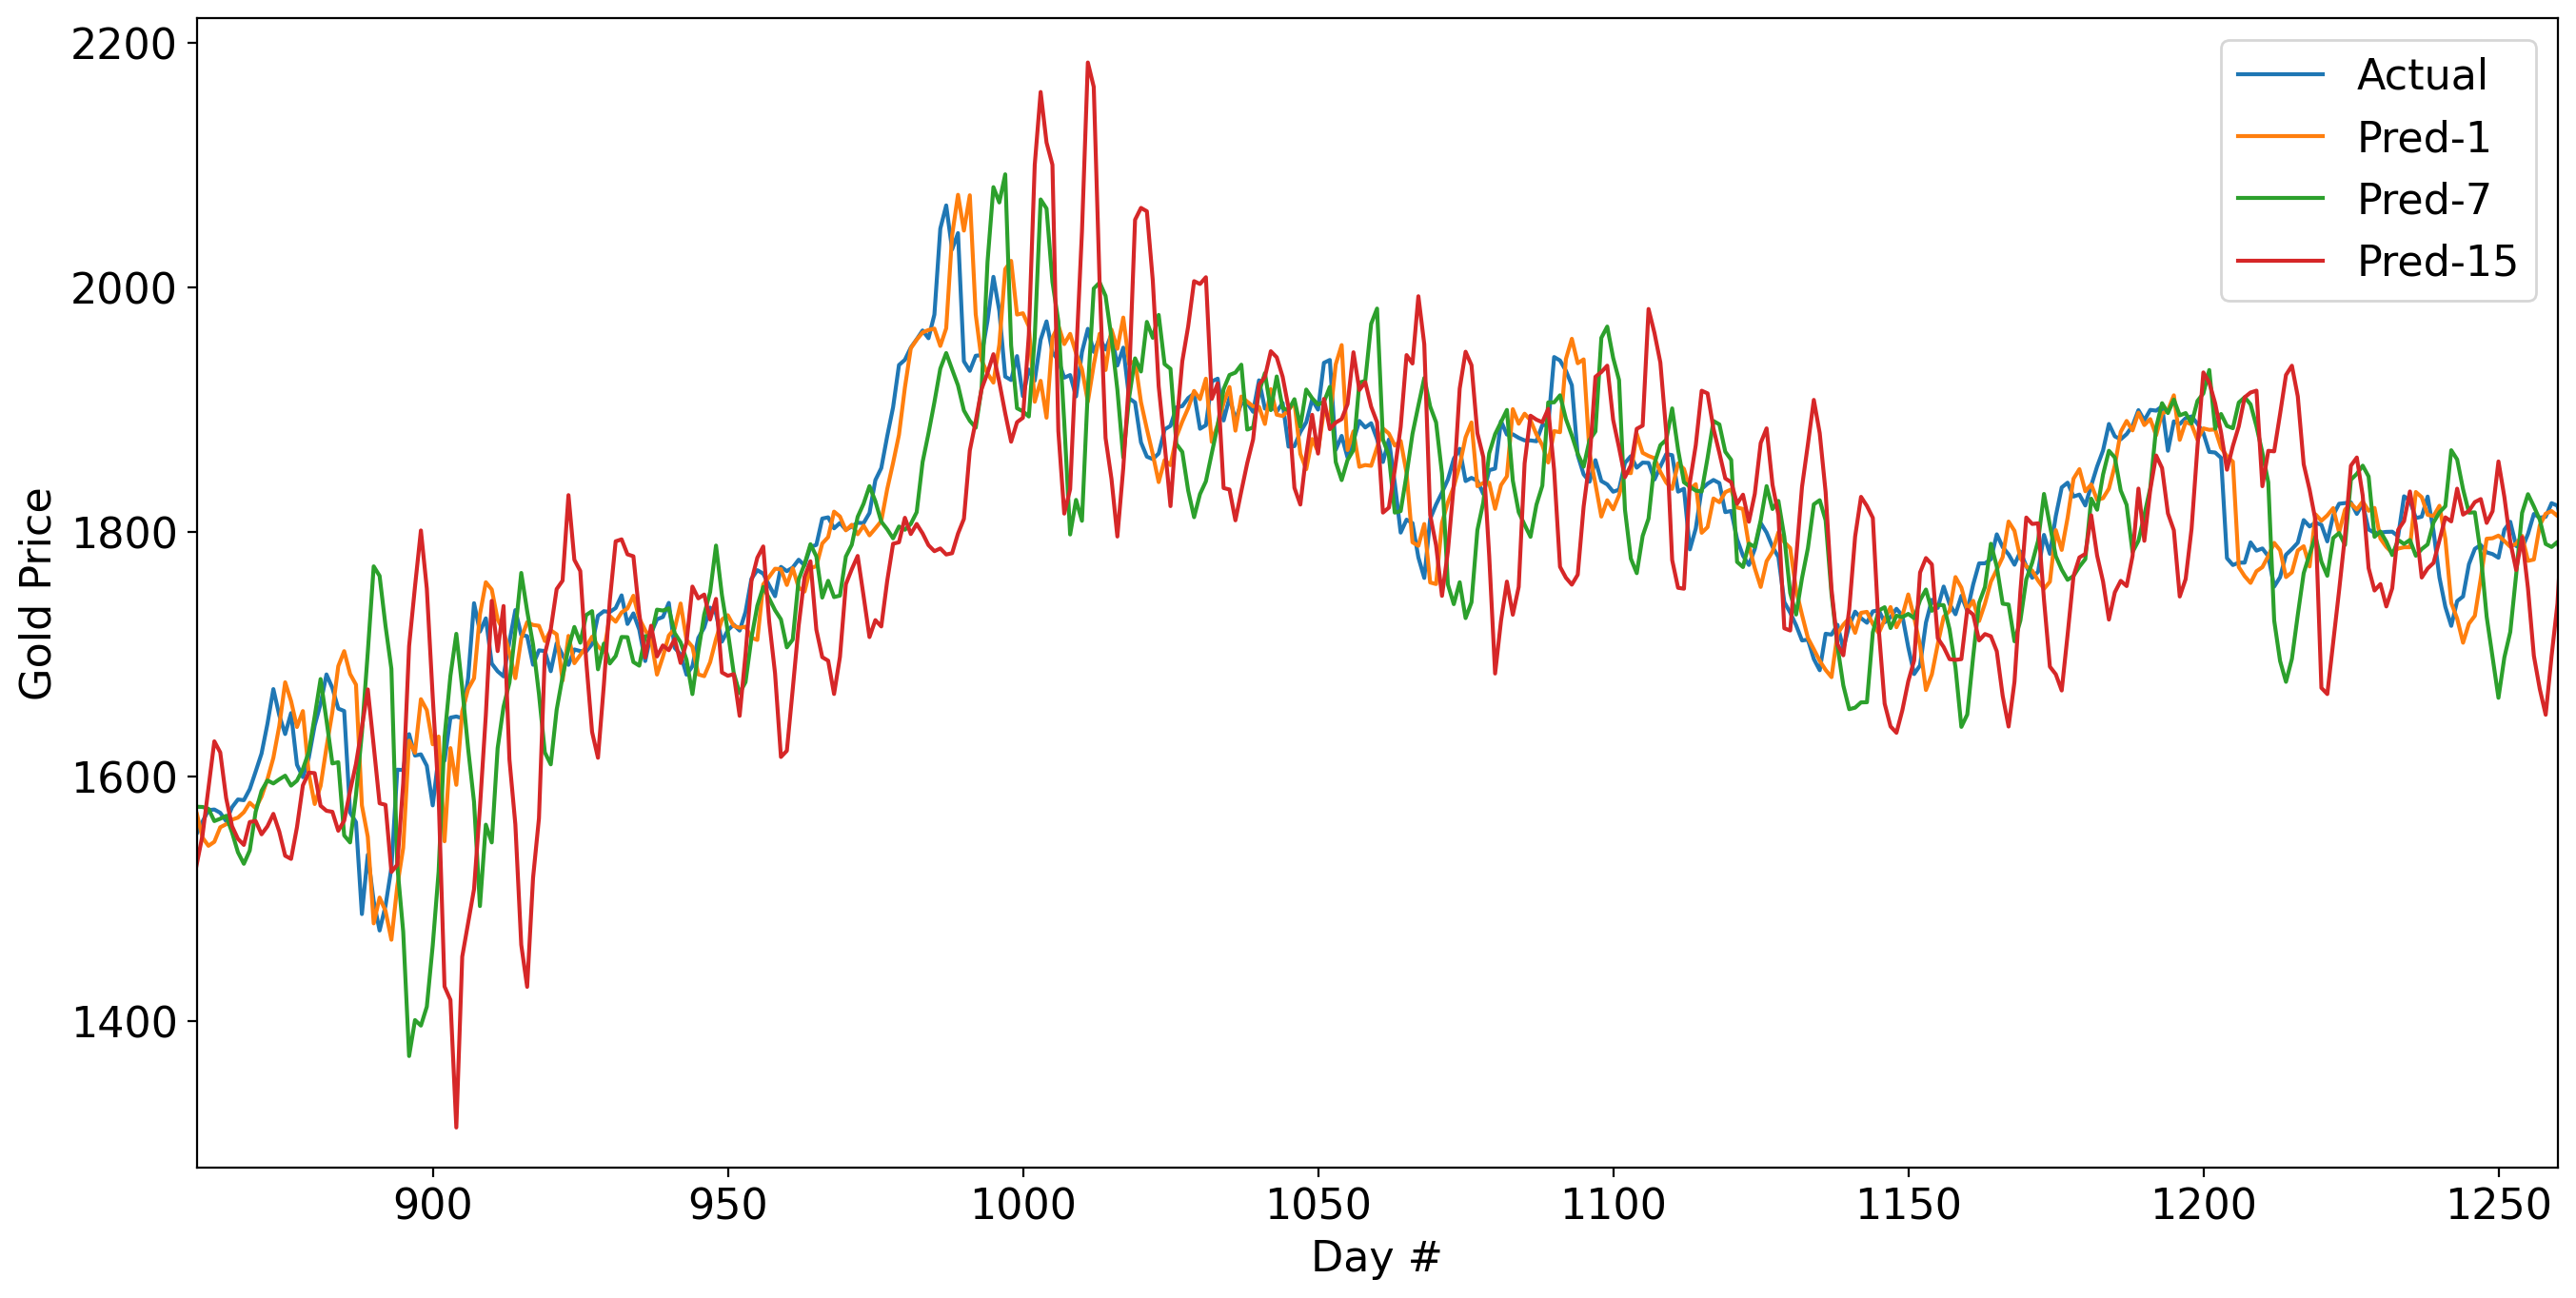
\includegraphics[width=8.1cm]{FinalGoldL}
		\centering 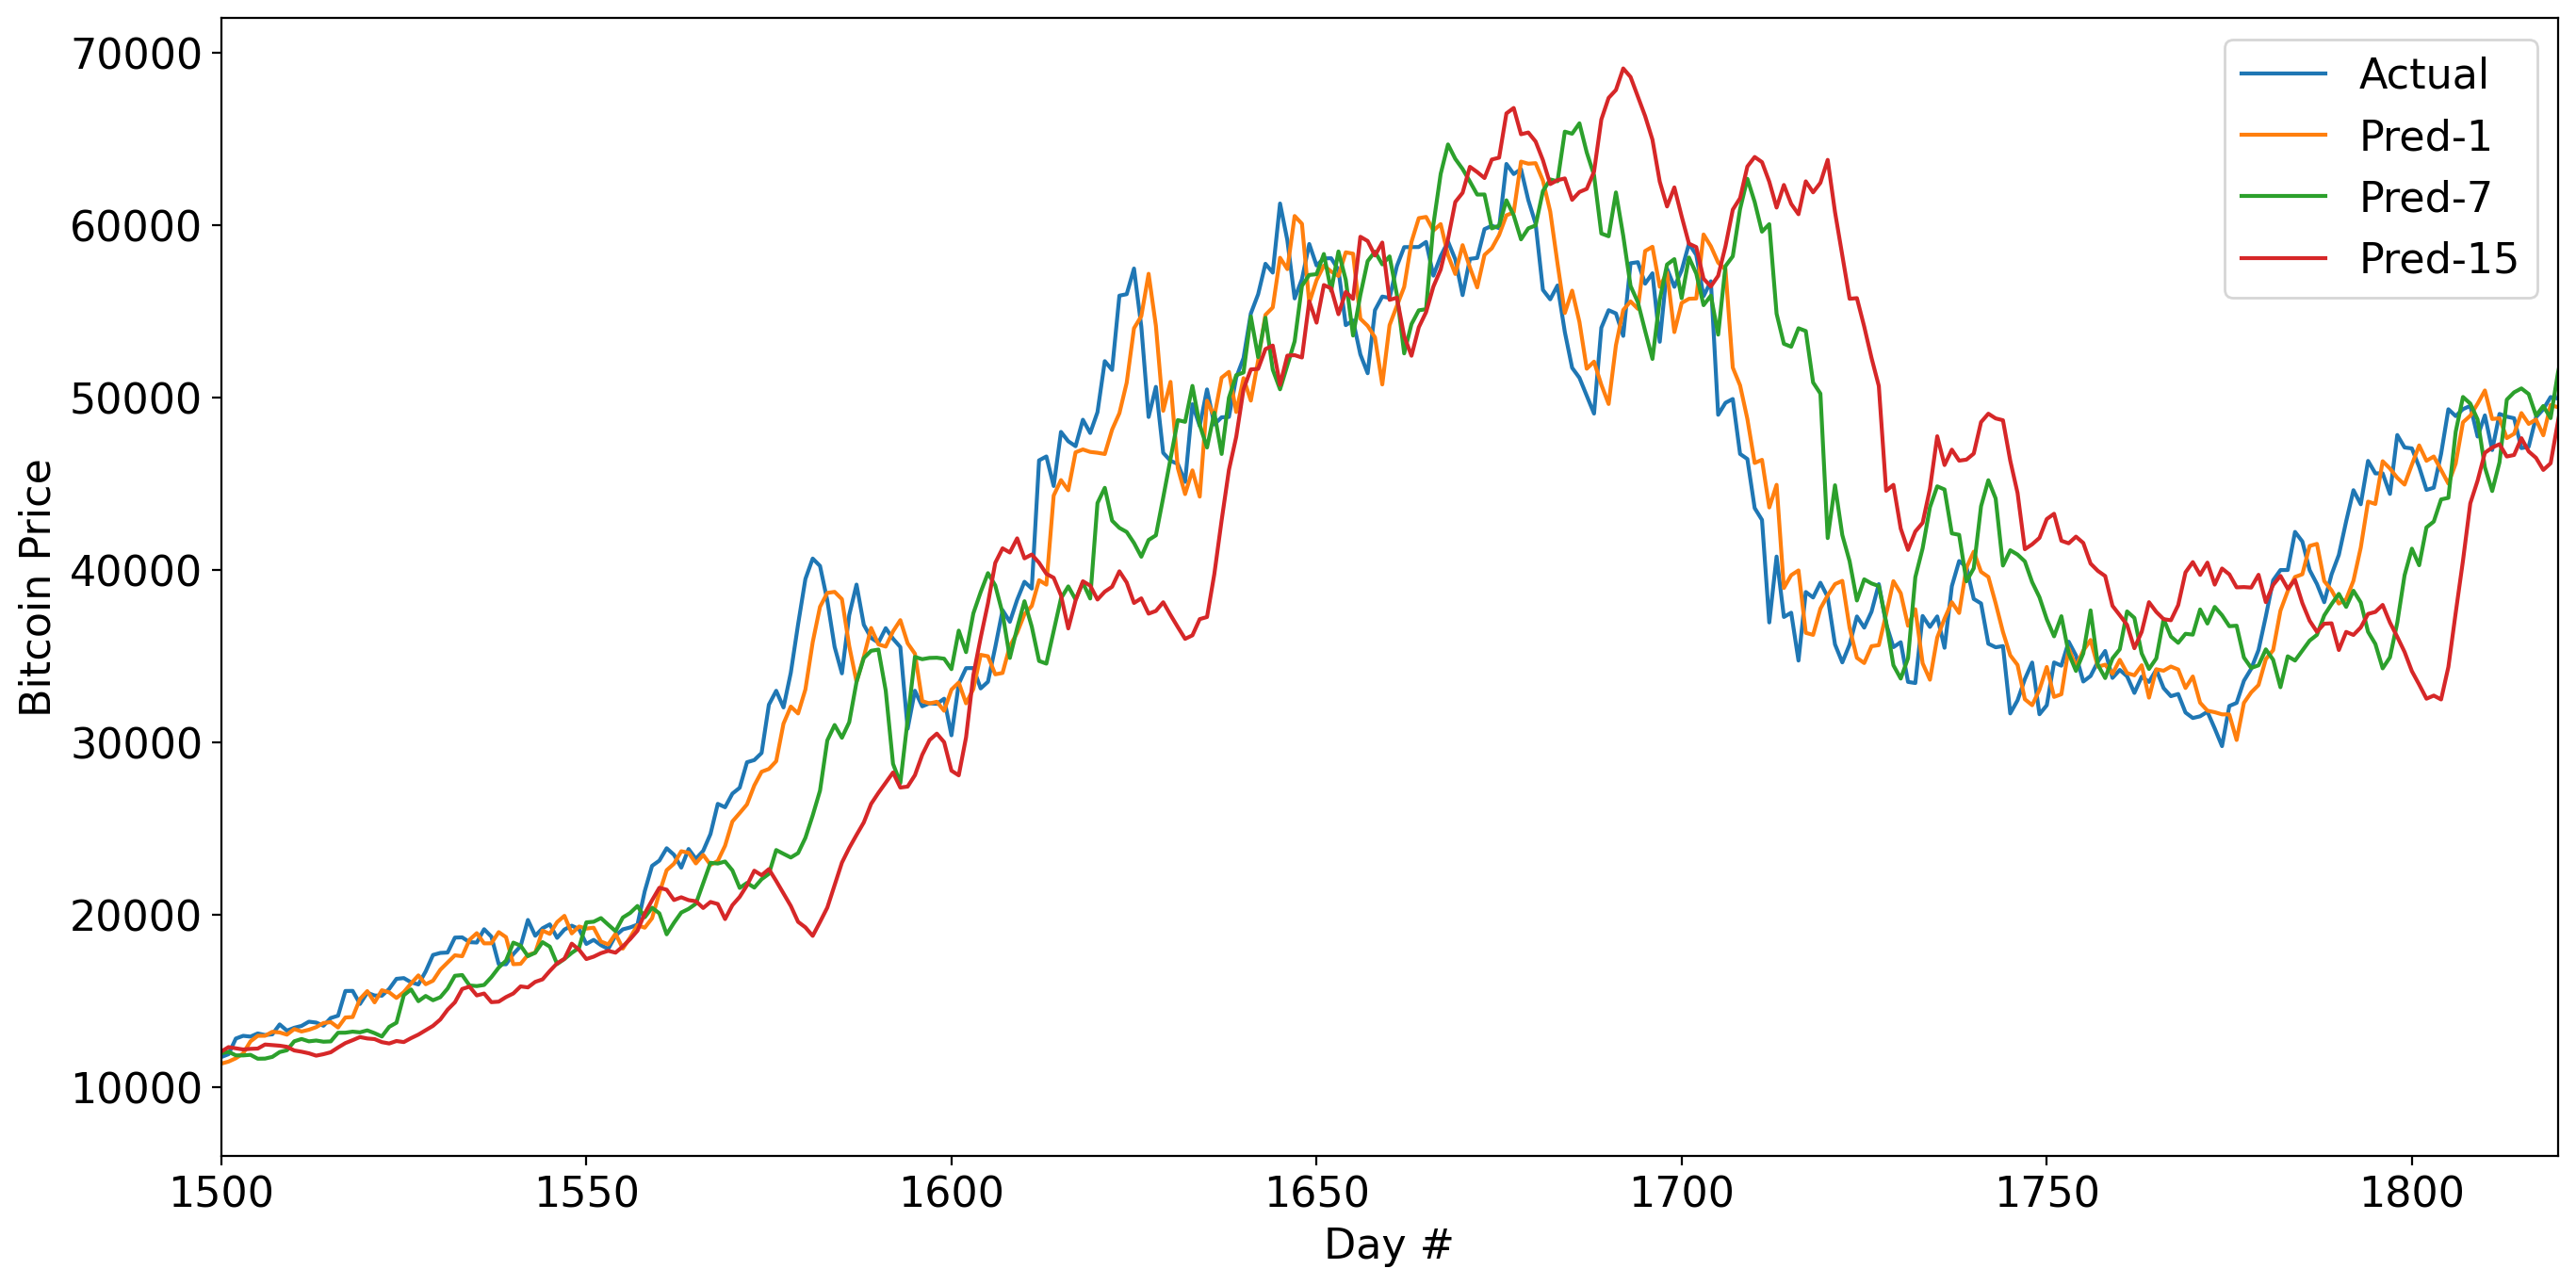
\includegraphics[width=8cm]{FinalBitcoinL}
		\caption{Long-term prediction of gold (left) and bitcoin (right) prices using \textbf{MLP MWF-15}}
	\end{figure}
	
	\newpage
	\section{Problem II: Designing An Investment Strategy}
	
	\subsection{Algorithm for Two Assets: Modified Capital Asset Pricing Model (CAPM)}
	\label{sec:4.1}
	
	We utilize the classical trading model, CAPM, to design our strategy. The key idea is to minimize the \textbf{Sharp ratio} (ratio of the expected profit rate to expected risk rate) as a two-variable function of trading volumes. Note that it is the \textit{ratio} -- rather than the magnitude of each rate -- that matters. 
	
	Using the results from Section \ref{sec:3.4}, we obtain predicted values of gold price after 1, 7, 15 days ($\hat{p}_{G+1}$, $\hat{p}_{G+7}$, $\hat{p}_{G+15}$). Setting the weights $\beta_1$, $\beta_2$, $\beta_3$ with AHP (methodology discussed in Section \ref{sec:4.3}), we take a weighted average of their growth rate relative to the current price $p_G$ to obtain an \textit{expected} profit rate of gold $E_G$. A similar technique is performed on the bitcoin prices. The total \textbf{profit rate} is obtained by dividing profit (commission fee deducted) by principal. 
	
	\begin{align}
		E_G & = \beta_1 \frac{\hat{p}_{G+1}-p_G}{p_G} + \beta_2 \frac{\hat{p}_{G+7}-p_G}{p_G} + \beta_3 \frac{\hat{p}_{G+15}-p_G}{p_G} \\
		E_B & = \beta_1 \frac{\hat{p}_{B+1}-p_B}{p_B} + \beta_2 \frac{\hat{p}_{B+7}-p_B}{p_B} + \beta_3 \frac{\hat{p}_{B+15}-p_B}{p_B} \\
		\textrm{Profit} & = \frac {E_G\left(G+\Delta G\right) + E_B\left(B+\Delta B\right) - \alpha_G|\Delta G| - \alpha_B|\Delta B|} {C+G+B}
	\end{align}
	
	The risk of an asset is closely related to the volatility of prices, which can be described by the standard deviation in the past 15 days ($\sigma_G$, $\sigma_B$). To strike a balance in the investment portfolio, the \textbf{risk rate} in the classical CAPM model also requires a correlation coefficient of the prices. The notation $\omega$ is introduced to conveniently represent the portion of gold in the total asset. 
	
	\begin{align}
		\sigma_G, \sigma_B & = \textrm{std} \left(p_{G-1}, p_{G-2}, \ldots, p_{G-15}\right), \textrm{std} \left(p_{B-1}, p_{B-2}, \ldots, p_{B-15}\right) \\
		\rho & = \frac {\textrm{Cov}\left(\left(p_{G-0}, p_{G-1}, \ldots, p_{G-15}\right), \left(p_{B-0}, p_{B-1}, \ldots, p_{B-15}\right)\right)} {\textrm{Var}\left(p_{G-0}, p_{G-1}, \ldots, p_{G-15}\right) \cdot \textrm{Var}\left(p_{B-0}, p_{B-1}, \ldots, p_{B-15}\right)} \\
		\omega & = \frac {G+\Delta G} {G+\Delta G+B+\Delta B} \\
		\textrm{Risk} & = {\sqrt{\omega^2 \sigma_G^2 + \left(1-\omega\right)^2 \sigma_B^2 + 2 \omega \left(1-\omega\right) \sigma_G \sigma_B \rho}}
	\end{align}

	Risk tolerance is a salient feature of investors and is called the Investor's Vulnerability Index $r$ in our model. Radical investors may have $r_R=0.1$, while $r_S=0.5$ depicts steadier behaviors. Higher risk means more \textit{potential} returns while cautiousness may guarantee a stable return. 
	
	The Sharp ratio $K$ is derived from the profit and risk rates. Note that the value of $r$ constraints the trading volumes $\Delta G$ and $\Delta B$, as the maximal portion of \textbf{risky assets} in total assets should not exceed a certain threshold determined by $r$ and the standard deviation of gold and bitcoin prices. \verb|scipy.optimize| is used as the optimizer. 
	
	\begin{align}
		G+\Delta G&+B+\Delta B \le (1-r\frac{\sigma_G+\sigma_B}{2})\left(C+G+B\right) \\
		K\left(\Delta G, \Delta B\right) & = \frac {\textrm{Profit}} {\textrm{Risk}} \\
		K\left(\Delta G_{opt}, \Delta B_{opt}\right) & = \mathop{\max}_{\Delta G, \Delta B} K\left(\Delta G, \Delta B\right)
	\end{align}
	
	Finally, the open interests of gold, bitcoin, and cash (\textbf{commission fee deducted}) are updated with the trading volumes and multiplied with the \textit{actual} growth rate before being substituted back into $C$, $G$, $B$ to continue the loop. This algorithm is repeated for the 1265 market days of gold. 
	
	\begin{align}
		G_{opt}, B_{opt} & = G + \Delta G_{opt}, B + \Delta B_{opt} \\
		C_{opt} & = C-\Delta G_{opt}-\Delta B_{opt}-\alpha_G\left|\Delta G_{opt}\right|-\alpha_B\left|\Delta B_{opt}\right| \\
		C, G, B & = C_{opt}, G_{opt} \frac{p_{G+1}}{p_G}, B_{opt} \frac{p_{B+1}}{p_B}
	\end{align}
	
	Yet there are 561 days in which only the bitcoin can be traded. Thus, it must be noticed that in these special cases, we utilize the \textbf{One-Variable Linear Programming} algorithm presented in Section \ref{sec:4.2}. Up till now, we are equipped with two sets of hyperparameters: $\beta_L$ versus $\beta_S$ controlling ``vision'', and $r_R$ versus $r_S$ controlling ``courage.'' The strategy turns out quite satisfying, achieving 3383.38\% in the 5-year period (equivalent to 103.42\% annually). Also, note that one will need more potential profit to compensate for being ``shortsighted'' than being overly cautious. 
	
	\begin{figure}[h]
		\label{fig:13}
		\centering 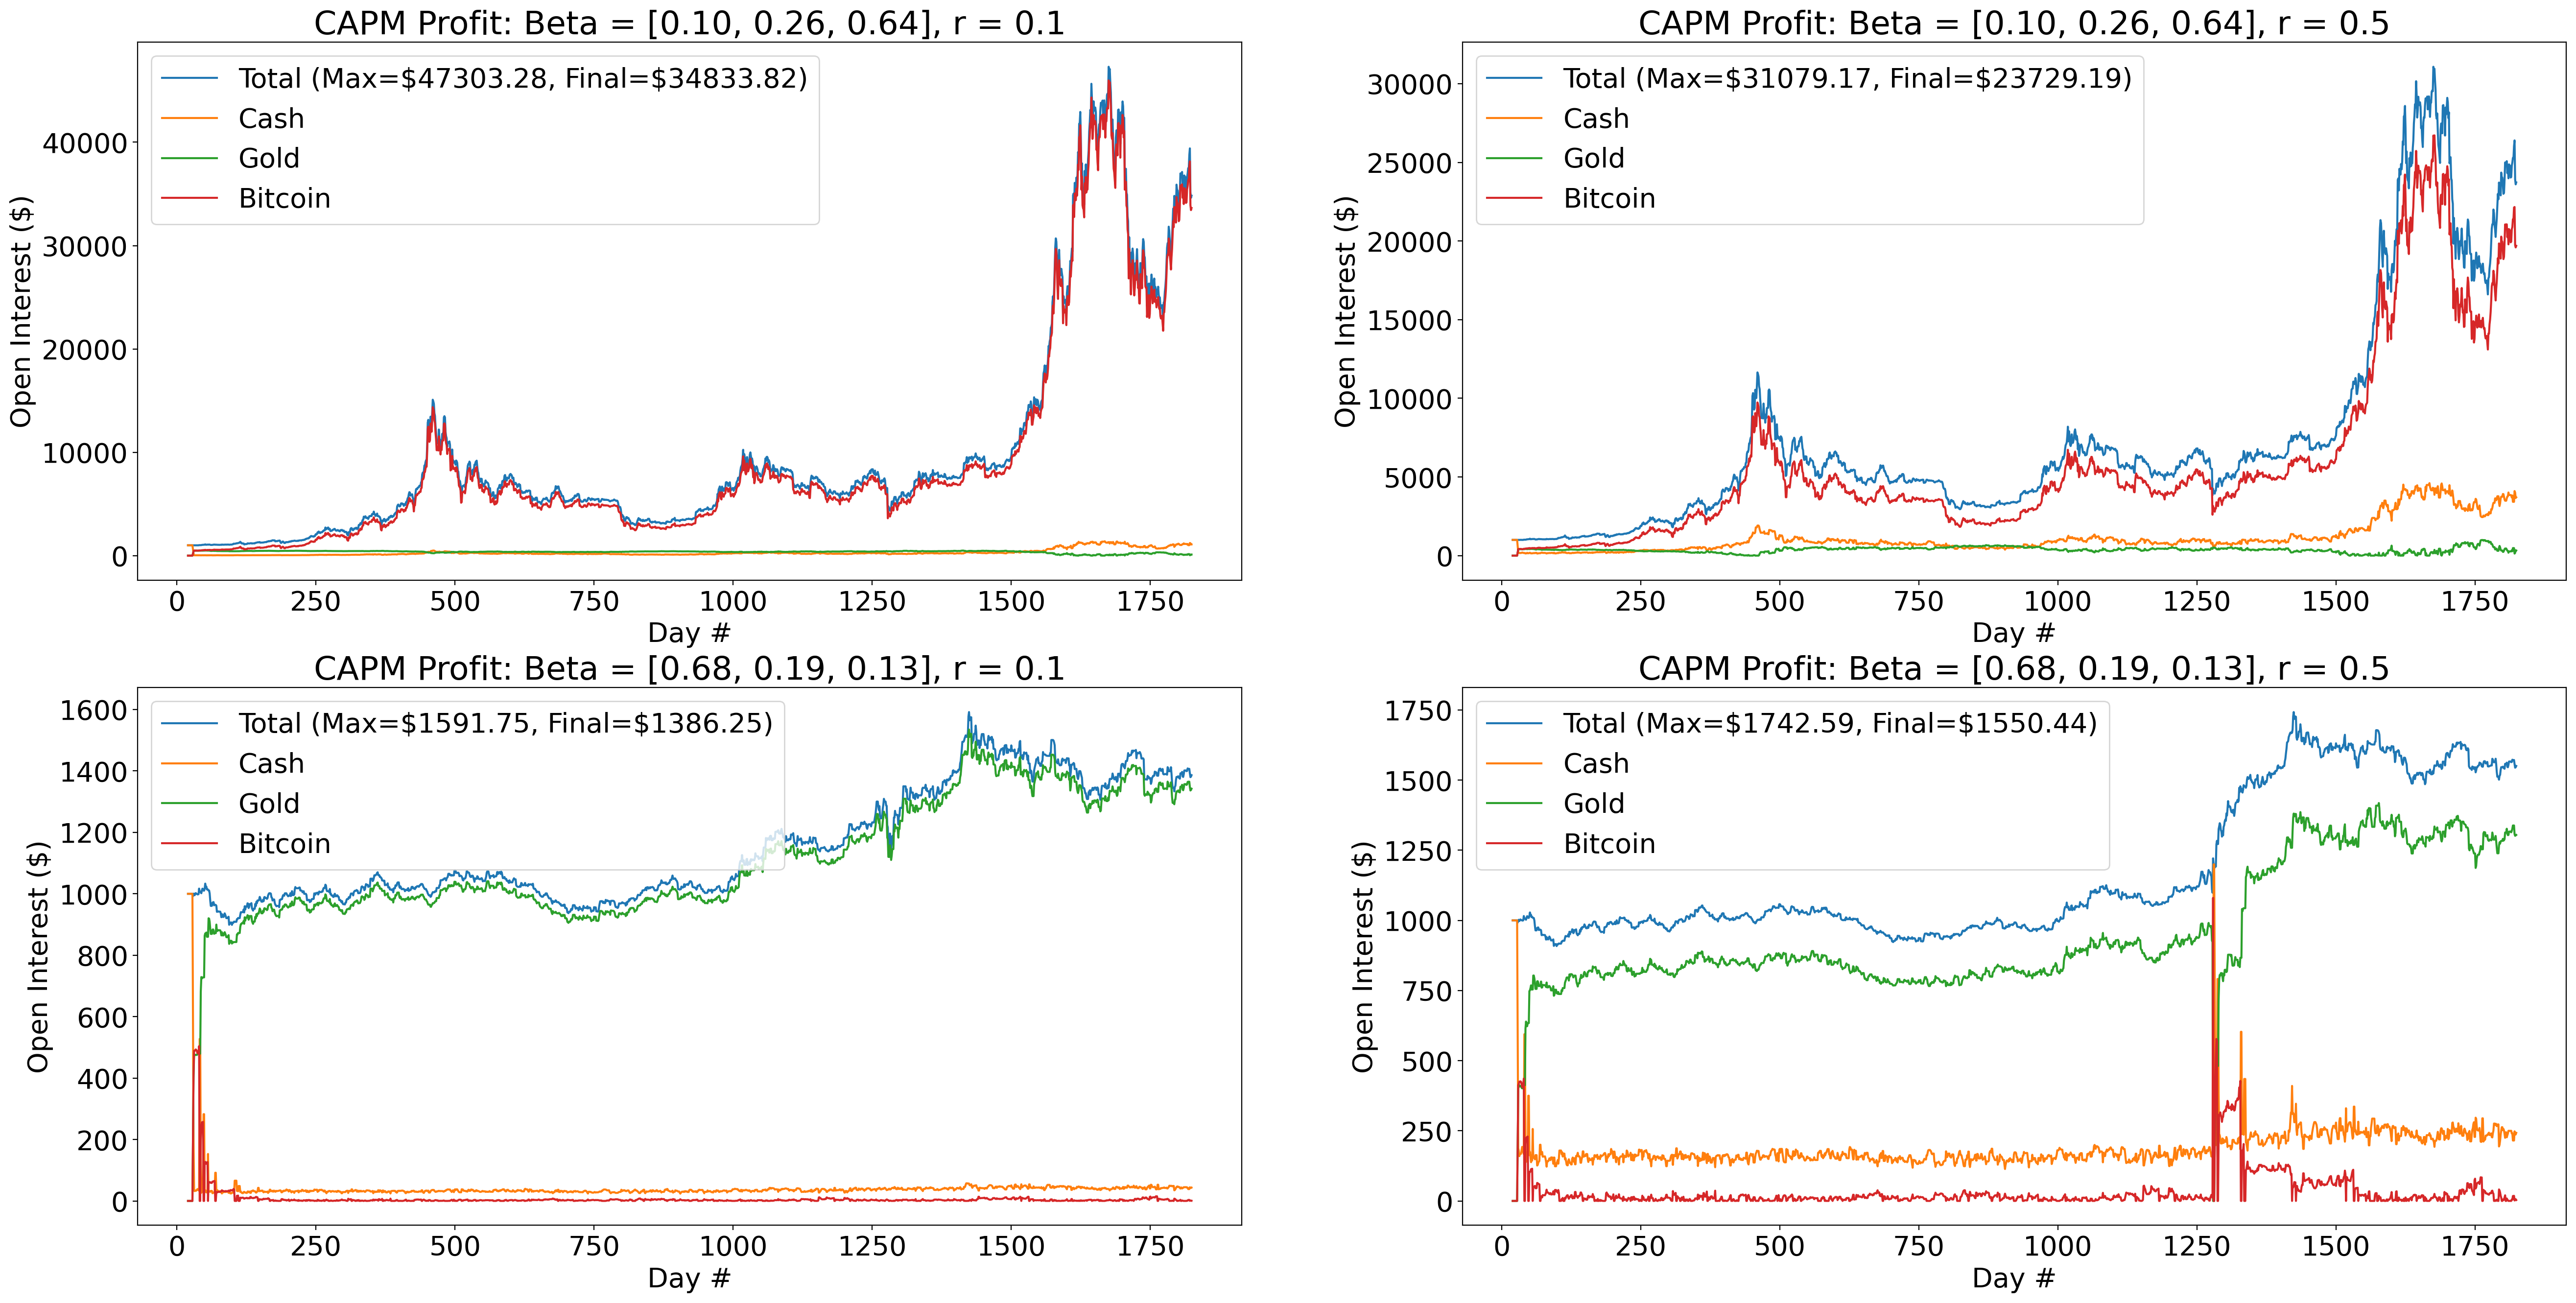
\includegraphics[width=16cm]{PREDCAPMWide}
		\caption{Profit and trading strategy of the gold-bitcoin portfolio using CAPM}
	\end{figure}
	
	\subsection{Algorithm for One Asset: Linear Programming (LinProg)}
	\label{sec:4.2}
	
	On the closing days of the gold market, CAPM becomes ineffective since it is impossible to invest in both gold and bitcoin. As a result, \textbf{linear programming} is specially designed for this situation. The Investor's Vulnerability Index $r$ is taken into account in addition to certain regular limit inequations. When the bitcoin risk rate rises, investors will alter their investment capital to mitigate the loss from the imposed high risk. This model performs more stably to environmental parameters and earns more profit than ceasing from operations when the gold market is closed. 
	
	Inheriting the variable names from Section \ref{sec:4.1}, when $E_B < \alpha_B$, the value of $\Delta B$ is obtained by solving the following linear programming problem: 
	
	$$
	\begin{aligned}
		\max \quad & E_B \Delta B - \alpha_B |\Delta B| \\
		\textrm{s.t.} \quad & \left\{
		\begin{aligned}
			& \Delta B + \alpha_B |\Delta B| < C \\
			& G + \Delta G + B + \Delta B < \left(1-r\sigma_B\right) \left(C+G+B\right) \\
			& B + \Delta B > 0
		\end{aligned}
		\right.
	\end{aligned}
	$$
	
	Otherwise, $\Delta B$ is directly calculated as $\Delta B = \max \left\{ \left( 1-r\sigma_B \right) \left(C+G+B\right) - G - B, 0 \right\}$. 
	
	\subsection{Determining the Hyperparameters: Analytic Hierarchy Process (AHP)}
	\label{sec:4.3}
	
	In our model, $\beta_x$ is a weight vector to determine the \textit{distribution of weight} among expected earnings. These weights may differ among investors due to variations in individual preference: some pay more attention to short-term returns while others emphasize long-term profits. Therefore, we build an AHP model to determine the weights of profit prediction for different kinds of investors. 
	
	We use predicted prices in 1, 7, 15 days to represent short-, medium-, and long-term returns to some extent. We first built evaluation matrices for different investors: the higher the ratio, the more important the factor. Specifically, since long-term returns are more appealing to long-term investors, the preference ratio over short-term returns is 7, which is much higher than 1. 
	
	\begin{table}[h]
		\centering
		\begin{tabular}{lccc}
			\toprule
			Benefits   & Short-term & Mid-term & Long-term \\ \midrule
			Short-term & $1$ & $1/2$ & $1/7$ \\
			Mid-term   & $2$ & $1$ & $1/2$ \\
			Long-term  & $7$ & $2$ & $1$ \\ \bottomrule
		\end{tabular}
		\caption{Evaluation matrix for long-term return chasers}
	\end{table}
	
	\begin{table}[h]
		\centering
		\begin{tabular}{lccc}
			\toprule
			Benefits   & Short-term & Mid-term & Long-term \\ \midrule
			Short-term & $1$ & $4$ & $5$ \\
			Mid-term   & $1/4$ & $1$ & $2$ \\
			Long-term  & $1/5$ & $1/2$ & $1$ \\ \bottomrule
		\end{tabular}
		\caption{Evaluation matrix for short-term return chasers}
	\end{table}
	
	Based on these two matrices, we calculate their maximal eigenvalues $\lambda_{\max}$. The corresponding eigenvectors $\textbf{\textrm{u}}=\left(u_{1}, u_{2}, u_{3}\right)^{\textrm{T}}$ are then normalized as below to obtain the weight vectors. 
	
	$$x_{i}=\frac{u_{i}}{\sum_{j=0}^{2} u_{j}}$$
	
	The vectors are $\beta_L = [0.10, 0.26, 0.64]$ for long-term and $\beta_S = [0.68, 0.19, 0.13]$ for short-term return chasers. The weights appear as $\beta_1$, $\beta_2$, and $\beta_3$ in Section \ref{sec:4.1}. 
	
	The evaluation matrices must pass \textbf{consistency check} for the results to be effective. Three popular indicators are the Coincidence Indicator and the Random Consistency Index: 
	
	\[ \mathrm{CI}=\frac{\lambda_{\max}-n}{n-1} \qquad \mathrm{RI}=\frac{\lambda^{\prime}_{\max}-n}{n-1} \qquad
	\mathrm{CR}=\frac{\mathrm{CI}}{\mathrm{RI}} \]
	
	The $ \mathrm{CR}$ values, both smaller than the threshold of $0.1$, are $0.034$ for long-term and $0.023$ for short-term return chasers. We can thus safely utilize the weight vectors as key factors in our model. 
	
	\section{Model Evaluation}
	\subsection{Sensitivity Analysis of Commission Rates}
	
	The commission fees, though being trivial at first sight, turn out to have dramatic effects on our final earnings, since the asset market is a so-called \textit{chaotic} system whose outcome can be significantly affected by small disturbances. For the four hyperparameter combinations -- $\beta_L$ (long-term vision) versus $\beta_S$ (short-term vision), $r_R$ (risky) versus $r_S$ (stable) -- we enumerate $\alpha_G \in \left( 0.005, 0.100 \right)$ and $\alpha_B \in \left( 0.020, 0.085 \right)$ to calculate CAPM results (\textbf{Shown in Figure \ref{fig:14}}). 
	
	In the long-term vision groups, the optimal earnings decrease in an approximately linear manner as $\alpha_G$ and $\alpha_B$ grow, and all the profits are maintained above \$30,000 for the risky strategy and \$15,000 for the steady strategy. Yet unexpected results arise in the short-term vision groups where maximal earning is achieved with the lowest $\alpha_G$ and the \textit{highest} $\alpha_B$. The behavior becomes even more irregular with the preference of stability over taking risks. This is possibly an indicator of the model lacking in robustness as its behavior varies unpredictably with changing hyperparameters. 
	
	\begin{figure}[h]
		\label {fig:14}
		\centering 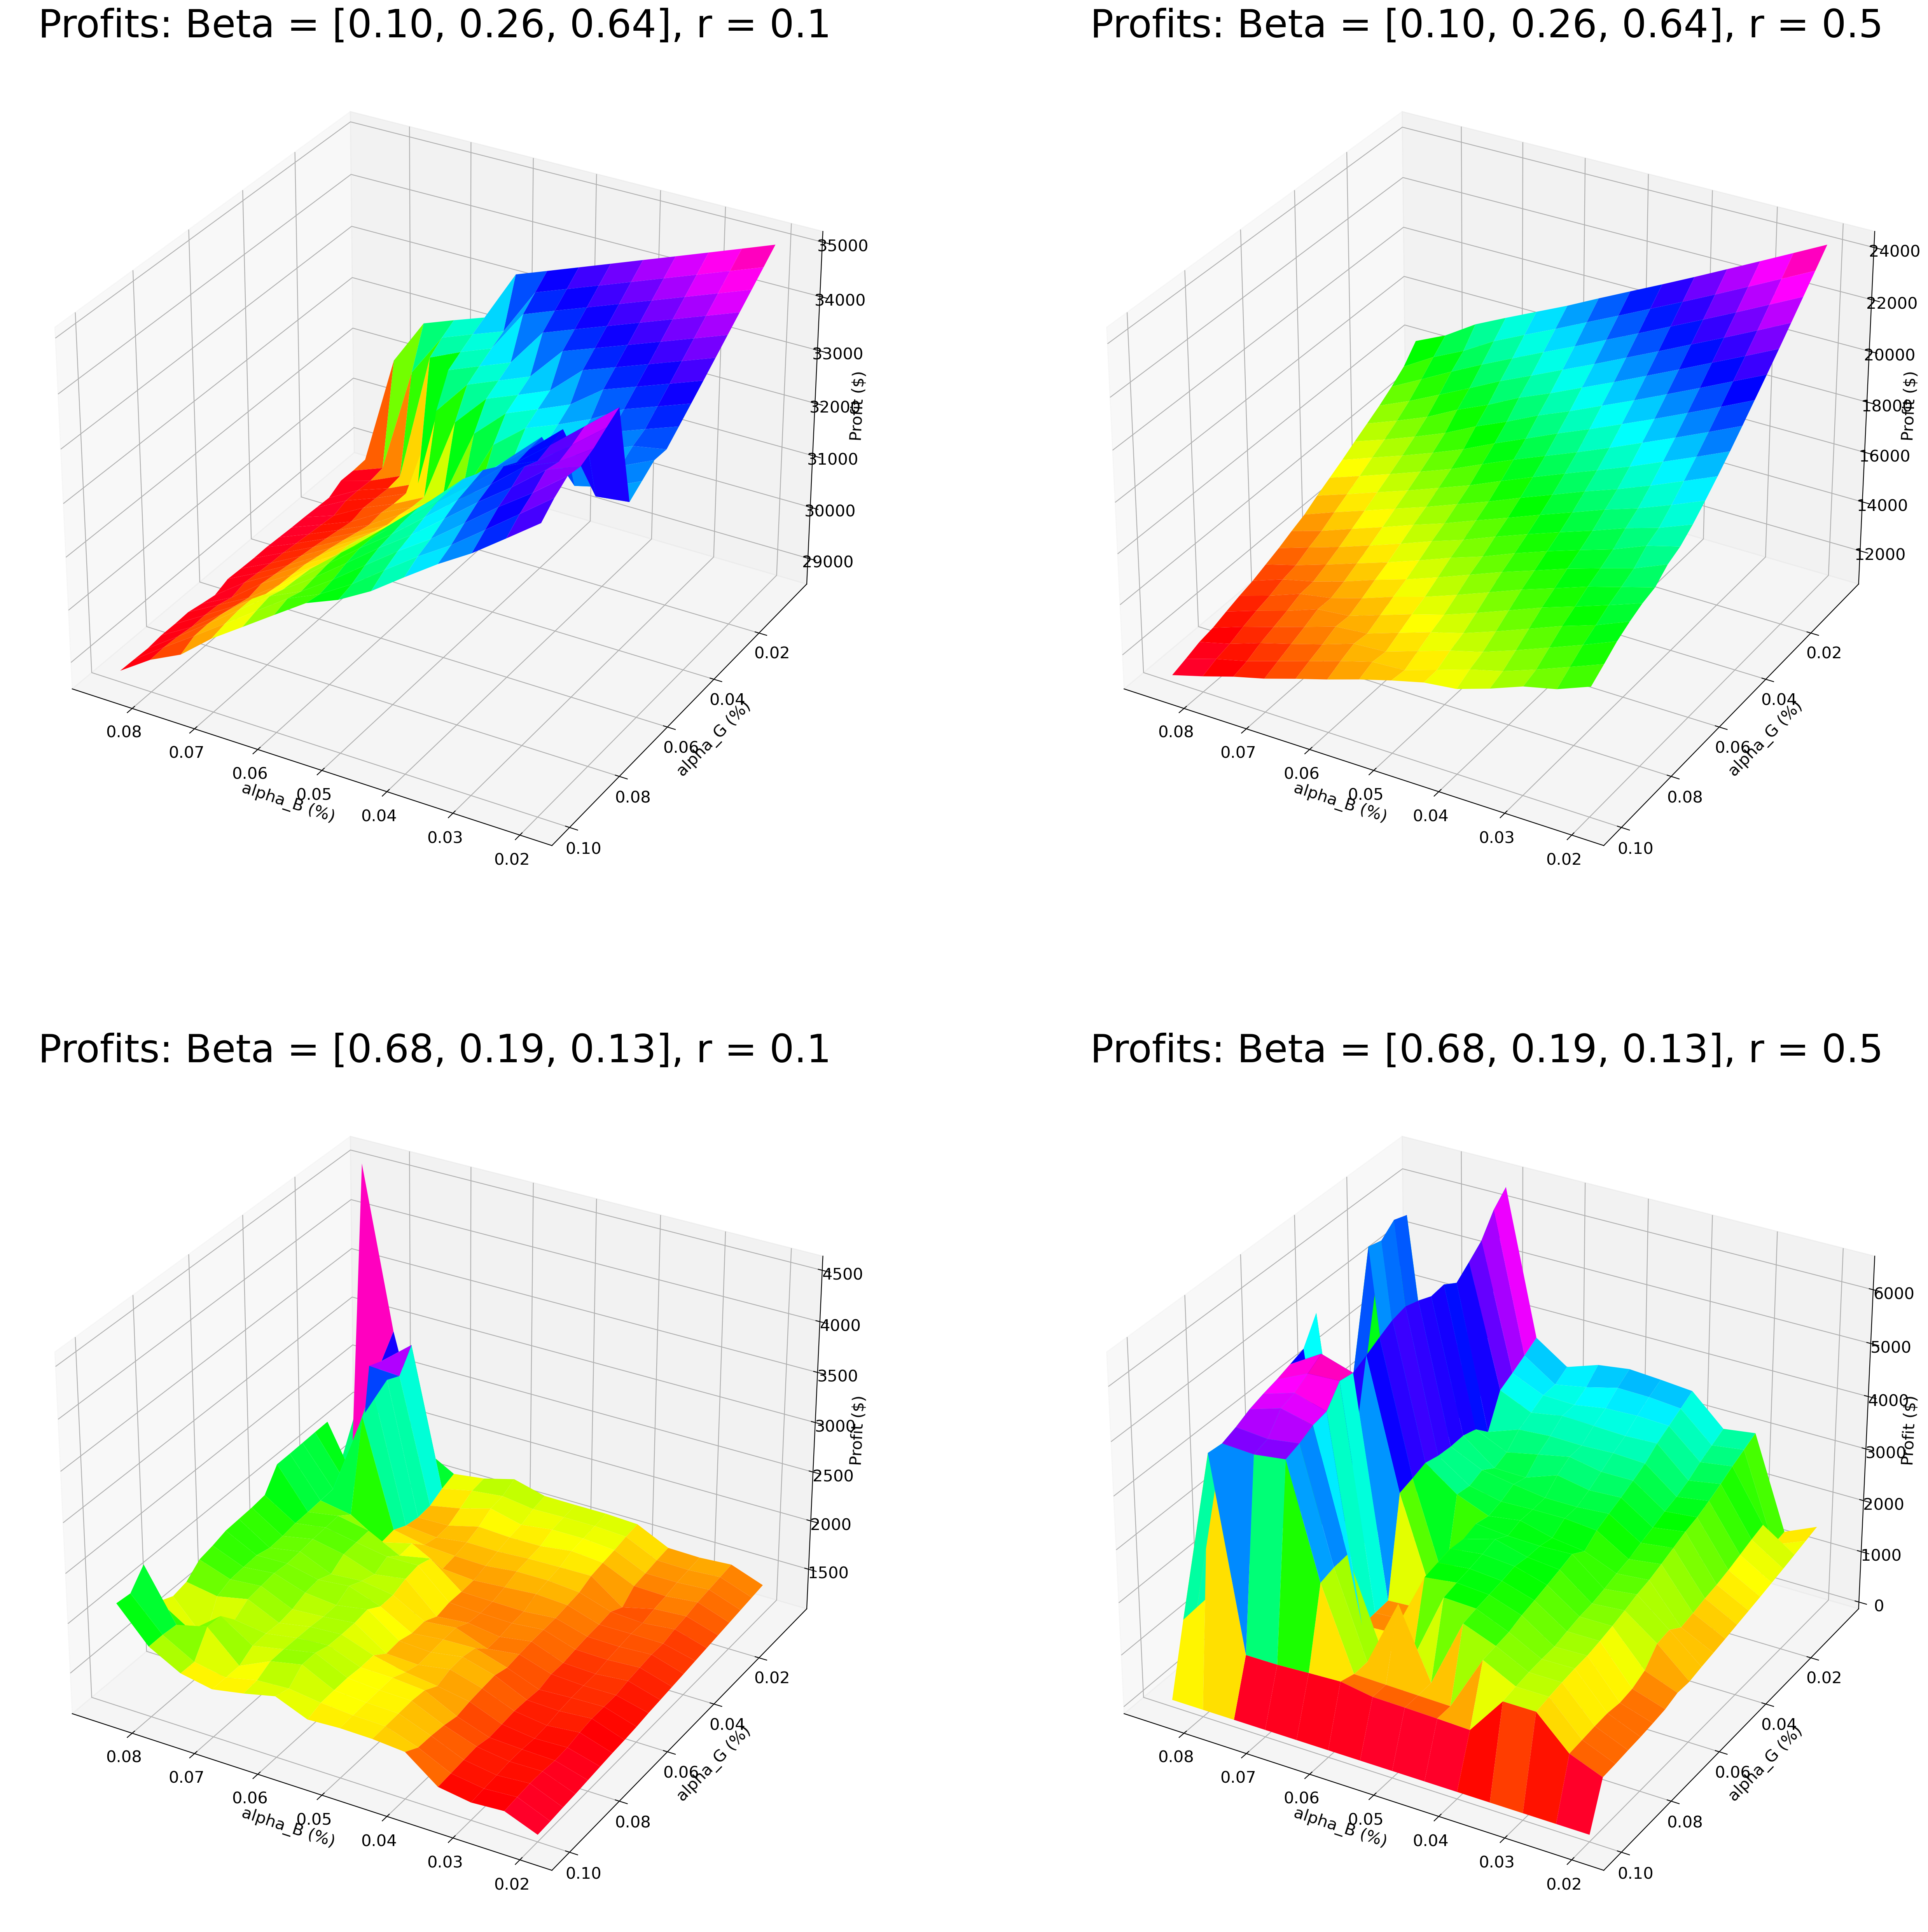
\includegraphics[width=16cm]{SensAnal}
		\caption{Profit and trading strategy of the gold-bitcoin portfolio using CAPM}
	\end{figure}
	
	\subsection{Evidence as the ``Best Strategy''}
	
	Our \textbf{prediction model} is carefully selected and crafted to achieve the highest prediction accuracy. Time series analysis algorithms like \textbf{ARIMA} are widely applied, yet it suffers from low predictive power in the long term (e.g., after 15 days) since it tends to make constant predictions outside the training range. \textbf{Neural networks} are capable of predicting long-term prices, provided that training data spanning multiple days (probably with dimension rising) is abundant. \textbf{Gray model}, on the contrary, requires much less training data than ARIMA and neural networks, but the predicted values sometimes blow up exponentially for higher-order GMs. Yet one interesting trait of GM is its capability of predicting \textit{trends} of future prices (refer to Figure \ref{fig:3} and \ref{fig:11}), which is especially powerful when investors apply the outperforming \textbf{risky strategy} (refer to Figure \ref{fig:13}). 
	
	~\\
	
	In terms of training data, \textbf{past data fitting} (PDF) is useful for suppressing outliers by focusing on predicting the trend from the entire set of historical data. However, the program runs slowlier as real-world data accumulates; besides, many neural networks do not accept a varied number of inputs, and \textbf{moving window fitting} (MWF) is introduced to counteract these side effects. Carefully weighing the pros and cons, we use \textbf{GM(1,1) PDF} for the first 10\% short-term predictions with insufficient data, and \textbf{MLP MWF-15} (member of the neural network family) for the other 90\% long-term predictions. 
	
	There is also evidence of our \textbf{decision model} outperforming other candidates. \textbf{CAPM} is widely regarded as one of the best strategies to guide investors to allocate their capital. Calculating the sharp rate $K$ allows inventors to determine the ideal asset-to-asset ratio. CAPM model shows strong robustness, performing well with different commission fee rates $\alpha$ and weight coefficients $\beta$ in the expected return rate. 
	
	An alternative approach is pure \textbf{Linear Programming} -- although one-variable LinProg assists CAPM at closed market days, two-variable LinProg completely replaces CAPM in this approach: 
	
	$$
	\begin{aligned}
		\max \quad & E_G \Delta G + E_B \Delta B - \alpha_G |\Delta G| - \alpha_B |\Delta B| \\
		\textrm{s.t.} \quad & \left\{
		\begin{aligned}
			& \Delta G + \Delta B + \alpha_G |\Delta G| + \alpha_B |\Delta B| < C \\
			& G + \Delta G + B + \Delta B < \left(1-r\frac{\sigma_G+\sigma_B}{2}\right) \left(C+G+B\right) \\
			& G + \Delta G > 0 \\
			& B + \Delta B > 0
		\end{aligned}
		\right.
	\end{aligned}
	$$
	
	At first sight, the model has a higher profit with certain parameters (\$55,287 with $\beta_L$ and $r_R$), yet it is extremely unstable when $\beta$ is altered and lacks the potential for extrapolation. In the worst case, this can yield \$30 (out of \$1,000) in the final trading day! 
	
	\begin{figure}[h]
		\centering 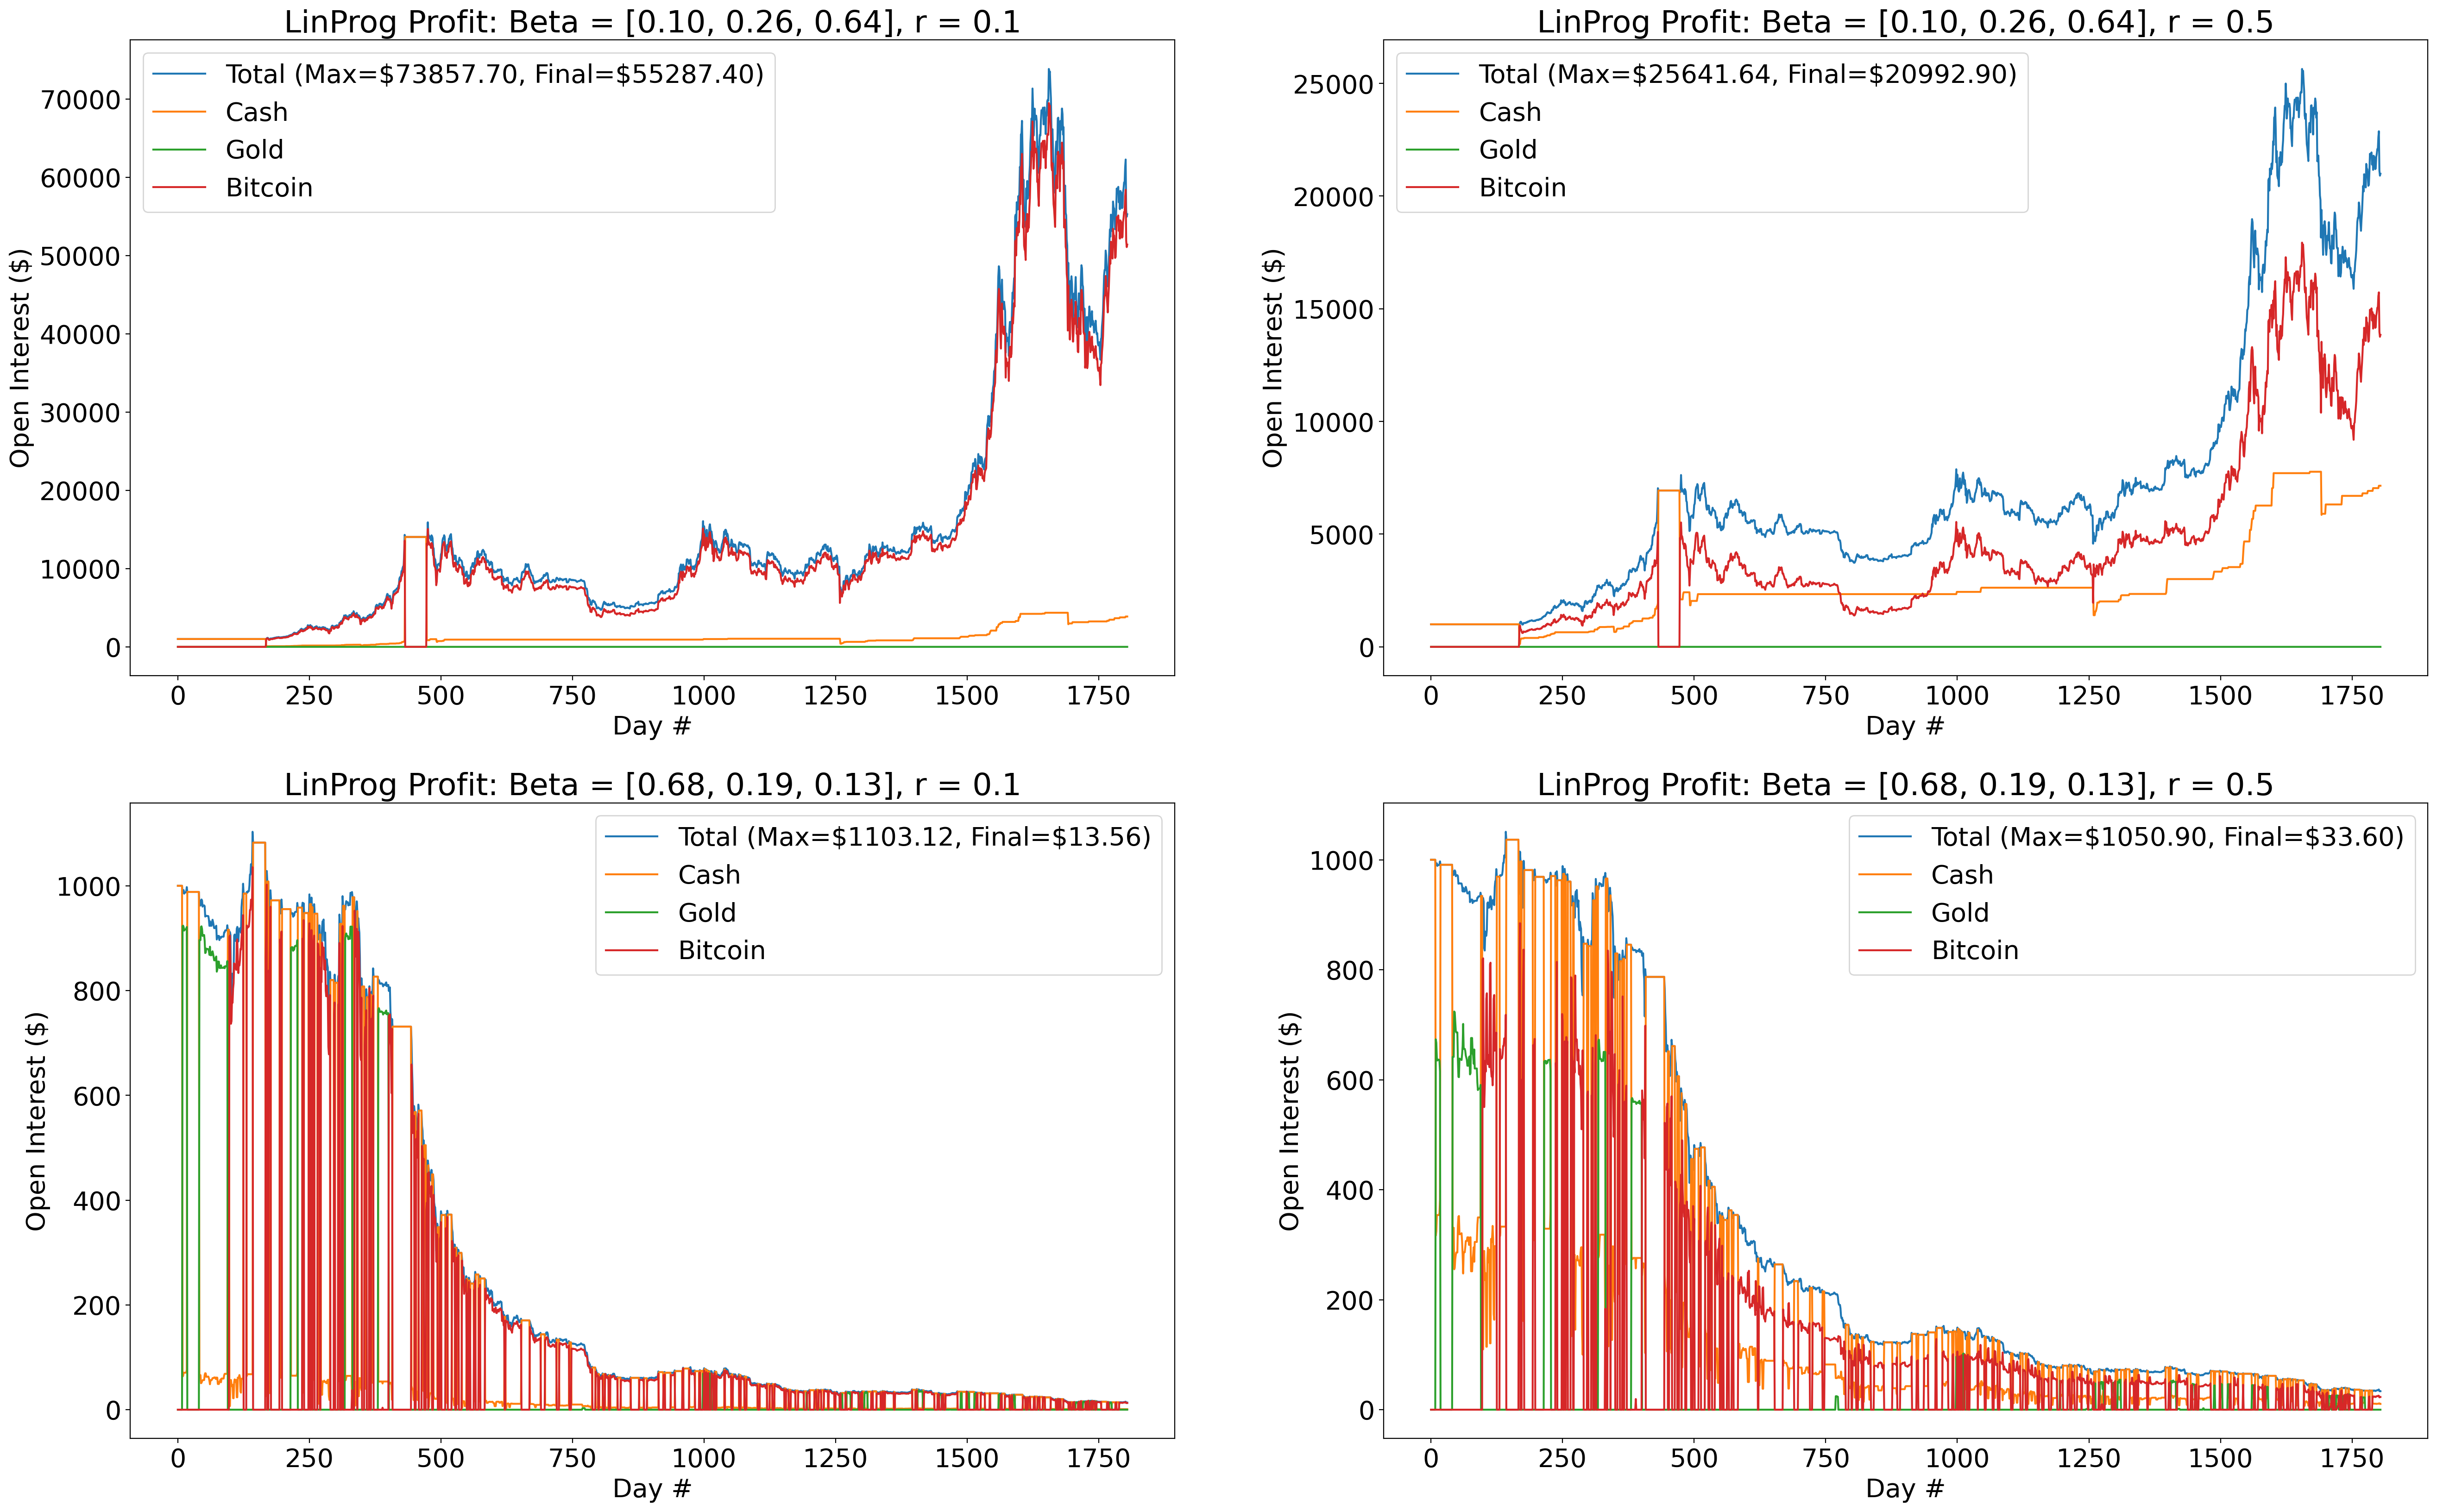
\includegraphics[width=16cm]{PREDLinProg}
		\caption{Profit and trading strategy of the gold-bitcoin portfolio using CAPM}
	\end{figure}
	
	The reality provides us with further evidence. Our annual bitcoin return rate of 103.42\% outperforms the average value of around 93.75\%, supporting that our strategy is one of the best. 
	
	\subsection{Directions for Further Research}
	
	\begin{itemize}
		\item In the prediction problem, the qualities of \textbf{little training data} and \textbf{long-term prediction} ability can hardly ever be achieved simultaneously. ARIMA and neural networks require large amounts of historical data, while GM's predicted values vary widely from the actual data due to exponential fitting. This calls for improved algorithms, such as LSTM with ``memories'' \cite{LSTM2}. 
		\item The issue of \textbf{time lag} is never completely solved. Except for GM, the models tend to make safe guesses -- even neural networks predict stabilizing values in a 15-day scope. Yet this issue seems tough to tackle: in the absence of ``circuit breakers'', even an experienced human analyzer can hardly make accurate predictions during volatile periods based solely on historical data. One potential fix is to rise data dimensions to include standard deviation. 
		\item Both CAPM and LP decision models experience certain degrees of \textbf{hypersensitivity}. As $m$ (investment ratio) varies, sometimes the \verb|scipy.optimize| function fails to converge. This indicates a lack of robustness and may hinder the model's wide application. 
	\end{itemize}
	
	\newpage
	\section{A Letter: Takeaway Points for Traders}
	
	Dear Mr. Trader: 
	
	According to your requirements, we have spent a lot of time and energy to complete this new investment strategy model. We are confident that as an expert in the field of investment, you are familiar with bitcoin and its instability, which we build a novel mathematical approach to combat. In this letter, we are pleased to share with you our algorithms for predicting gold and bitcoin price data as well as the strategy for allocating your capital. We believe our models can optimize the return while minimizing the risk to the greatest extent possible. Here is how to figure out whether to stock, open, or close a position on any given day. 
	
	In order to make an accurate price estimation, we divide the period between 2016 to 2021 into two stages. At the former stage (roughly from 9/12/2016 to 5/27/2017), we strongly recommend you to utilize the \textbf{Gray Model} to predict the price data of bitcoin and gold, since it provides us with a price prediction with higher precision (absolute error rate: 1.0\%~5.8\%) when the historical data is insufficient. Furthermore, it can also offer you a decent picture of price changing several days later. After 5/27/2017, when available price data accumulates, you can make use of the \textbf{Neural Network} for data prediction such as MLP (Multiple Layer Perception). 
	
	When compared to the traditional time series method, \textbf{ARIMA} (Autoregressive Integrated Moving Average model), which only gives good performance for short-term predictions, MLP provides us with a higher price prediction accuracy than the Gray Model not only for short-term prices but also for long-term ones if it is trained with sufficient data, Overall, the average precision of anticipated price data (one day ahead) with our prediction model is greater than 98\%. 
	
	\begin{center}
		\begin{tabular}{l|cccc}
			\toprule
			& Gold $R^2$ & Gold Error & Bitcoin $R^2$ & Bitcoin Error \\ \midrule
			Pred 1 day & 0.9915 & 1.0338\% & 0.9049 & 3.9053\% \\
			Pred 7 days & 0.9639 & 2.1376\% & 0.8833 & 4.8204\% \\
			Pred 15 days & 0.9277 & 3.1739\% & 0.8159 & 6.4166\% \\
			\bottomrule
		\end{tabular}
	\end{center}
	
	After getting reliable forecasted price data, we develop an updated \textbf{CAPM} (Capital Asset Pricing Model) to help you deploy your capital into these two assets. The major flaw for traditional CAPM is that the expected return rate is hard to calculate, especially for assets with high risk, bitcoin being one of them. The advantages of our model are presented as follows. 
	
	Before making decisions, we will first predict the price values for bitcoin and gold for one, seven, and fifteen days, considering both short-term and long-term earnings. These accurately anticipated values with adjustable yet fair weight can be used to establish the final \textbf{expected earnings}. Plus, we have also taken into account the \textbf{risk ``appetite''} of our users. If our consumer is willing to take on more risk, they can adjust the \textbf{Risk Vulnerability Index} \textbf{$r$} to a smaller degree; if they are prudent, they may select a larger value to avoid potential loss. We give the users with several modes as a result of these properties. They have the option of becoming a long-term risk-tolerant investor or a short-term conservative trader. There is an essential idea in the financial industry that all investment agents should allow customers to make judgments, and our model is sufficiently adaptable to meet the needs of a wide range of users. 
	
	Based on the relatively accurate prediction model and the unique decision model, our strategy performed well on the investment deals. Our model can typically make \$1000 into \$20,000 to \$40,000 in 5 years, with the annual interest rate surpassing 100\%. For those who are long-term profit chasers with a higher risk appetite, our model can help them make even more! 
	
	\begin{figure}[h]
		\centering 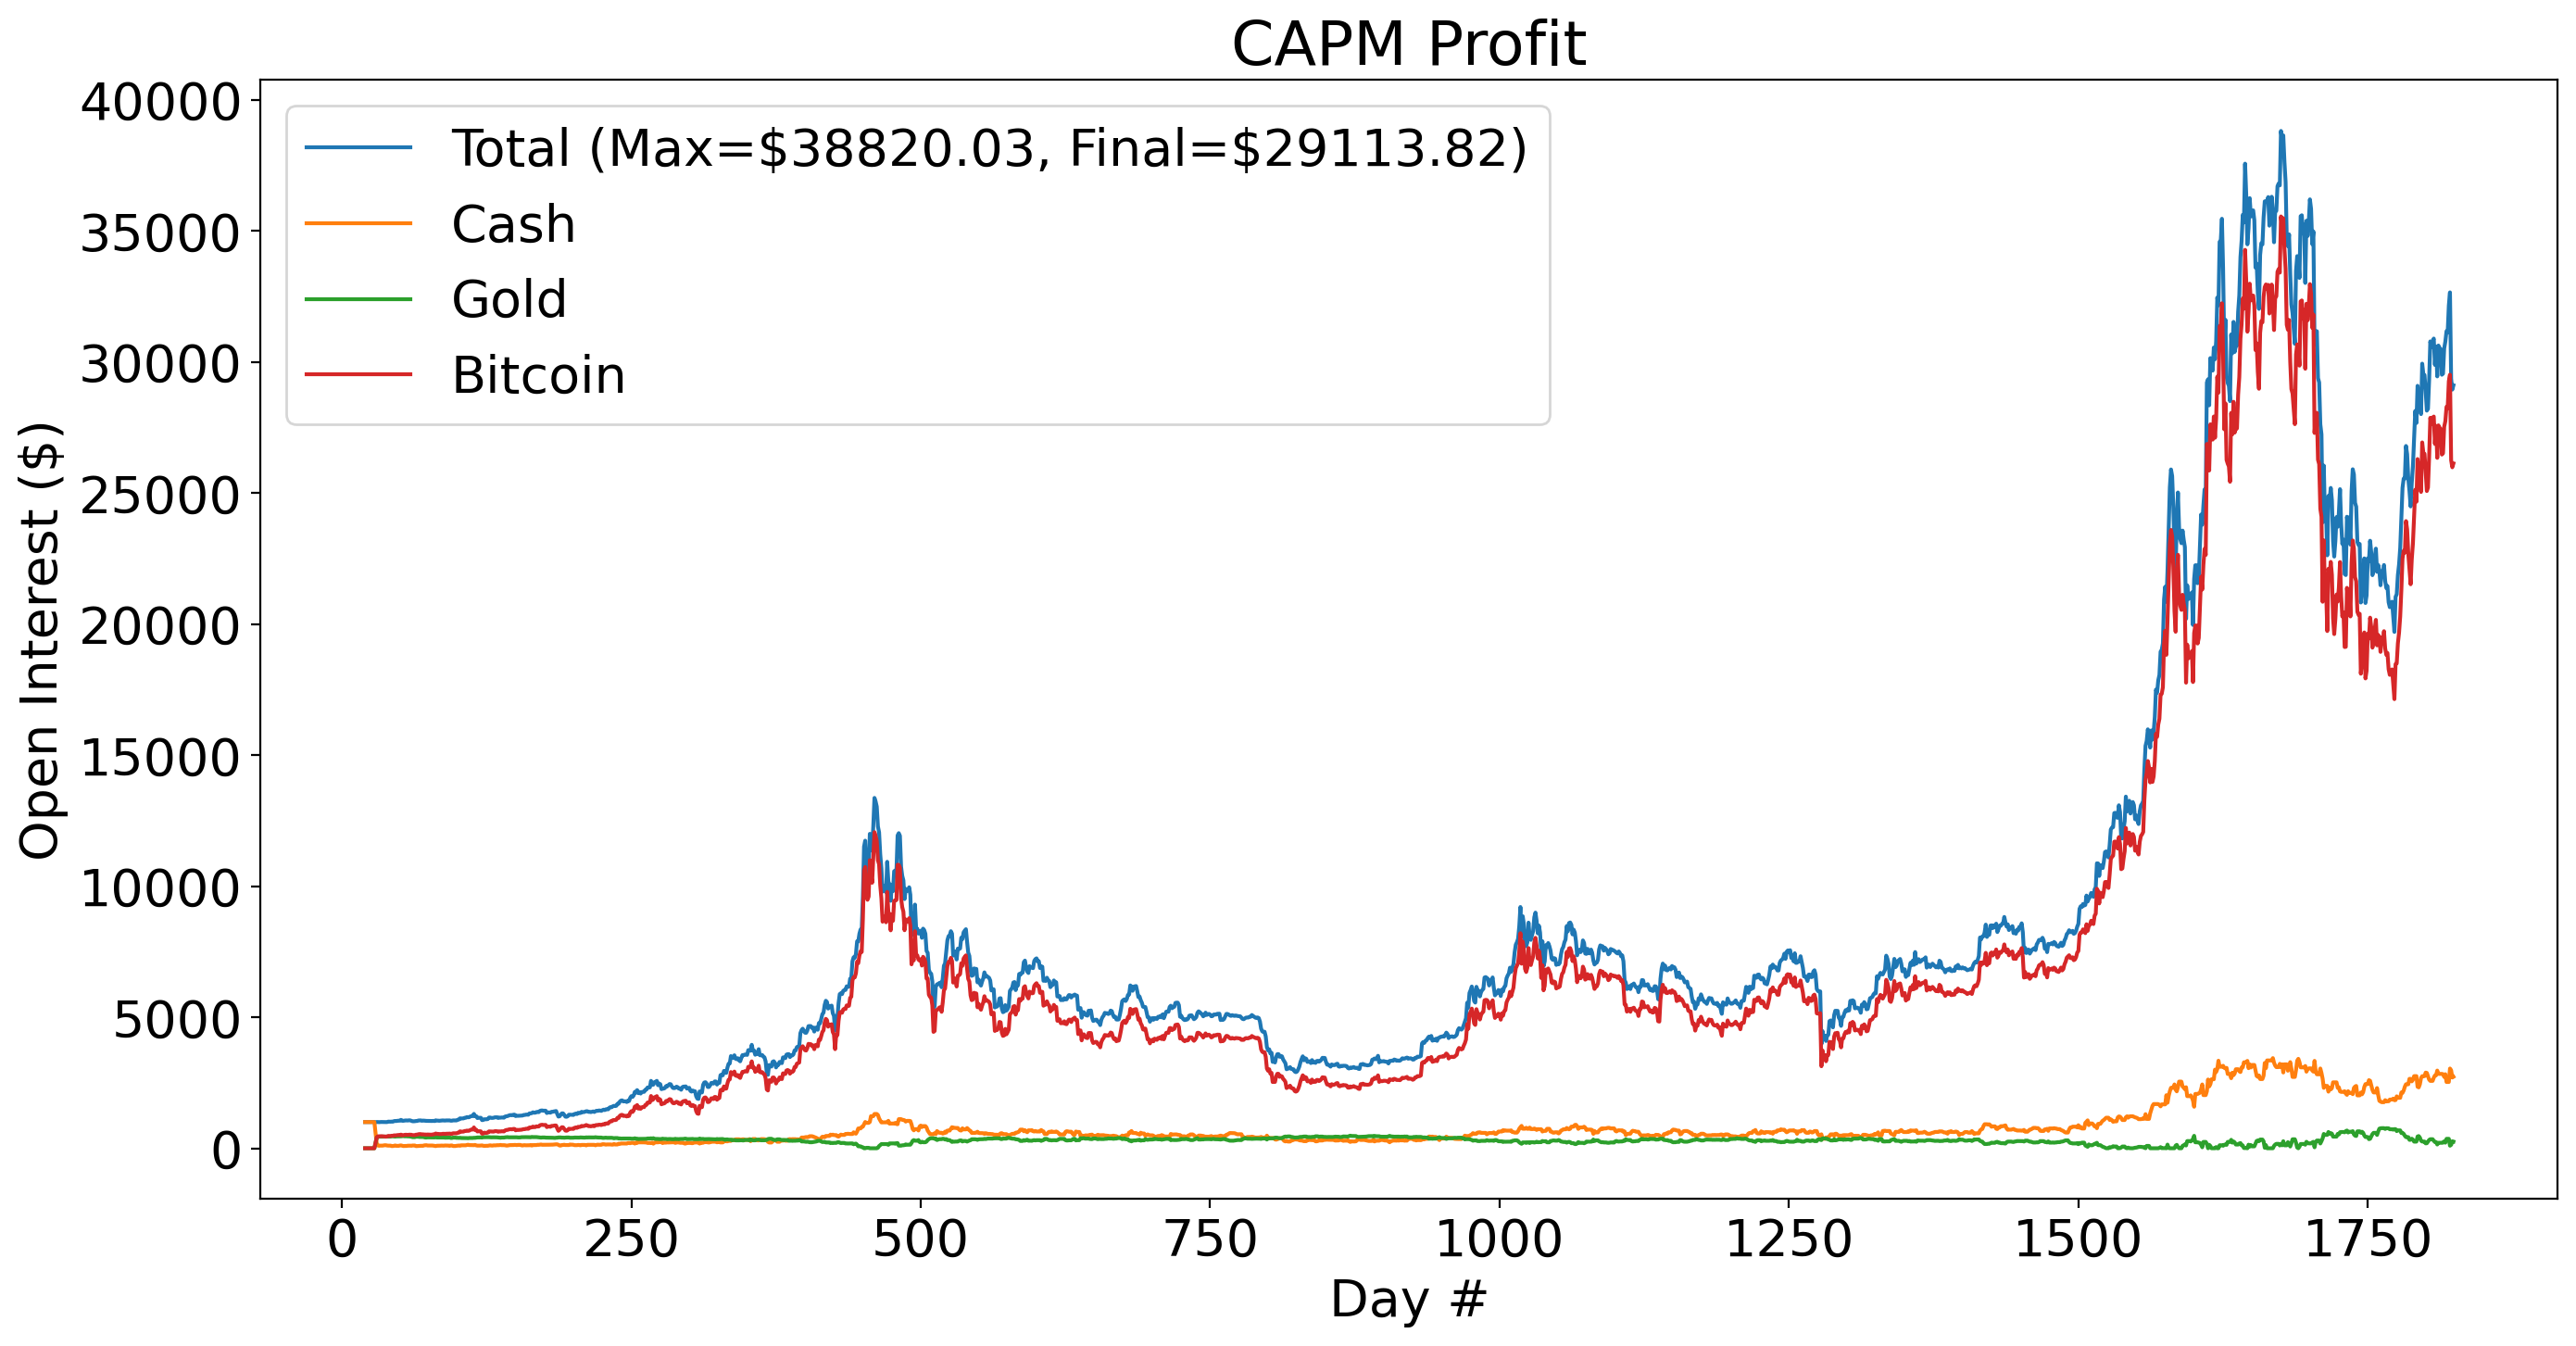
\includegraphics[width=16cm]{PREDLetter}
		\caption{Profit and trading strategy of the gold-bitcoin portfolio using CAPM}
	\end{figure}
	
	This model is flexible under different situations. It will be hard for the changing environment to stop our users from getting a profit. We are convinced that it can strongly assist you in your work to deal with different investors' requirements. It is our sincere hope that you can appreciate it. \\[12pt]
	
	\rightline{Best wishes,}
	
	\rightline{The Team of MCM}
	
	\newpage
	\bibliographystyle{plain}
	\bibliography{2214713_Reference}
	\newpage
	
\end{document}